\documentclass[twoside]{book}

% Packages required by doxygen
\usepackage{calc}
\usepackage{doxygen}
\usepackage{graphicx}
\usepackage[utf8]{inputenc}
\usepackage{makeidx}
\usepackage{multicol}
\usepackage{multirow}
\usepackage{fixltx2e}
\PassOptionsToPackage{warn}{textcomp}
\usepackage{textcomp}
\usepackage[nointegrals]{wasysym}
\usepackage[table]{xcolor}

% Font selection
\usepackage[T1]{fontenc}
\usepackage{mathptmx}
\usepackage[scaled=.90]{helvet}
\usepackage{courier}
\usepackage{amssymb}
\usepackage{sectsty}
\renewcommand{\familydefault}{\sfdefault}
\allsectionsfont{%
  \fontseries{bc}\selectfont%
  \color{darkgray}%
}
\renewcommand{\DoxyLabelFont}{%
  \fontseries{bc}\selectfont%
  \color{darkgray}%
}
\newcommand{\+}{\discretionary{\mbox{\scriptsize$\hookleftarrow$}}{}{}}

% Page & text layout
\usepackage{geometry}
\geometry{%
  a4paper,%
  top=2.5cm,%
  bottom=2.5cm,%
  left=2.5cm,%
  right=2.5cm%
}
\tolerance=750
\hfuzz=15pt
\hbadness=750
\setlength{\emergencystretch}{15pt}
\setlength{\parindent}{0cm}
\setlength{\parskip}{0.2cm}
\makeatletter
\renewcommand{\paragraph}{%
  \@startsection{paragraph}{4}{0ex}{-1.0ex}{1.0ex}{%
    \normalfont\normalsize\bfseries\SS@parafont%
  }%
}
\renewcommand{\subparagraph}{%
  \@startsection{subparagraph}{5}{0ex}{-1.0ex}{1.0ex}{%
    \normalfont\normalsize\bfseries\SS@subparafont%
  }%
}
\makeatother

% Headers & footers
\usepackage{fancyhdr}
\pagestyle{fancyplain}
\fancyhead[LE]{\fancyplain{}{\bfseries\thepage}}
\fancyhead[CE]{\fancyplain{}{}}
\fancyhead[RE]{\fancyplain{}{\bfseries\leftmark}}
\fancyhead[LO]{\fancyplain{}{\bfseries\rightmark}}
\fancyhead[CO]{\fancyplain{}{}}
\fancyhead[RO]{\fancyplain{}{\bfseries\thepage}}
\fancyfoot[LE]{\fancyplain{}{}}
\fancyfoot[CE]{\fancyplain{}{}}
\fancyfoot[RE]{\fancyplain{}{\bfseries\scriptsize Generated on Wed Oct 1 2014 11\+:37\+:41 for Wildlife\+Capture by Doxygen }}
\fancyfoot[LO]{\fancyplain{}{\bfseries\scriptsize Generated on Wed Oct 1 2014 11\+:37\+:41 for Wildlife\+Capture by Doxygen }}
\fancyfoot[CO]{\fancyplain{}{}}
\fancyfoot[RO]{\fancyplain{}{}}
\renewcommand{\footrulewidth}{0.4pt}
\renewcommand{\chaptermark}[1]{%
  \markboth{#1}{}%
}
\renewcommand{\sectionmark}[1]{%
  \markright{\thesection\ #1}%
}

% Indices & bibliography
\usepackage{natbib}
\usepackage[titles]{tocloft}
\setcounter{tocdepth}{3}
\setcounter{secnumdepth}{5}
\makeindex

% Custom commands
\newcommand{\clearemptydoublepage}{%
  \newpage{\pagestyle{empty}\cleardoublepage}%
}


%===== C O N T E N T S =====

\begin{document}

% Titlepage & ToC
\pagenumbering{roman}
\begin{titlepage}
\vspace*{7cm}
\begin{center}%
{\Large Wildlife\+Capture }\\
\vspace*{1cm}
{\large Generated by Doxygen 1.8.7}\\
\vspace*{0.5cm}
{\small Wed Oct 1 2014 11:37:41}\\
\end{center}
\end{titlepage}
\clearemptydoublepage
\tableofcontents
\clearemptydoublepage
\pagenumbering{arabic}

%--- Begin generated contents ---
\chapter{Namespace Index}
\section{Packages}
Here are the packages with brief descriptions (if available)\+:\begin{DoxyCompactList}
\item\contentsline{section}{{\bf com} }{\pageref{namespacecom}}{}
\item\contentsline{section}{{\bf com.\+securics} }{\pageref{namespacecom_1_1securics}}{}
\item\contentsline{section}{{\bf com.\+securics.\+wildlifecapture} }{\pageref{namespacecom_1_1securics_1_1wildlifecapture}}{}
\end{DoxyCompactList}

\chapter{Hierarchical Index}
\section{Class Hierarchy}
This inheritance list is sorted roughly, but not completely, alphabetically\+:\begin{DoxyCompactList}
\item \contentsline{section}{com.\+securics.\+wildlifecapture.\+Activity\+Debug}{\pageref{classcom_1_1securics_1_1wildlifecapture_1_1_activity_debug}}{}
\item Callback\begin{DoxyCompactList}
\item \contentsline{section}{com.\+securics.\+wildlifecapture.\+Camera\+Preview}{\pageref{classcom_1_1securics_1_1wildlifecapture_1_1_camera_preview}}{}
\end{DoxyCompactList}
\item \contentsline{section}{com.\+securics.\+wildlifecapture.\+Perspective\+Transformation\+Engine}{\pageref{classcom_1_1securics_1_1wildlifecapture_1_1_perspective_transformation_engine}}{}
\item Runnable\begin{DoxyCompactList}
\item \contentsline{section}{com.\+securics.\+wildlifecapture.\+Main\+Activity.\+Auto\+Code\+Runner\+Runnable}{\pageref{classcom_1_1securics_1_1wildlifecapture_1_1_main_activity_1_1_auto_code_runner_runnable}}{}
\item \contentsline{section}{com.\+securics.\+wildlifecapture.\+Main\+Activity.\+Auto\+Focus\+Runnable}{\pageref{classcom_1_1securics_1_1wildlifecapture_1_1_main_activity_1_1_auto_focus_runnable}}{}
\item \contentsline{section}{com.\+securics.\+wildlifecapture.\+Main\+Activity.\+Burst\+Checker\+Runnable}{\pageref{classcom_1_1securics_1_1wildlifecapture_1_1_main_activity_1_1_burst_checker_runnable}}{}
\item \contentsline{section}{com.\+securics.\+wildlifecapture.\+Main\+Activity.\+Burst\+Runnable}{\pageref{classcom_1_1securics_1_1wildlifecapture_1_1_main_activity_1_1_burst_runnable}}{}
\item \contentsline{section}{com.\+securics.\+wildlifecapture.\+Main\+Activity.\+Push\+To\+J\+N\+I\+Runnable}{\pageref{classcom_1_1securics_1_1wildlifecapture_1_1_main_activity_1_1_push_to_j_n_i_runnable}}{}
\end{DoxyCompactList}
\item \contentsline{section}{com.\+securics.\+wildlifecapture.\+Size\+Calculation\+Data}{\pageref{classcom_1_1securics_1_1wildlifecapture_1_1_size_calculation_data}}{}
\item Activity\begin{DoxyCompactList}
\item \contentsline{section}{com.\+securics.\+wildlifecapture.\+Documentation}{\pageref{classcom_1_1securics_1_1wildlifecapture_1_1_documentation}}{}
\item \contentsline{section}{com.\+securics.\+wildlifecapture.\+Main\+Activity}{\pageref{classcom_1_1securics_1_1wildlifecapture_1_1_main_activity}}{}
\end{DoxyCompactList}
\item Async\+Task\begin{DoxyCompactList}
\item \contentsline{section}{com.\+securics.\+wildlifecapture.\+Main\+Activity.\+Save\+Photo\+Task}{\pageref{classcom_1_1securics_1_1wildlifecapture_1_1_main_activity_1_1_save_photo_task}}{}
\end{DoxyCompactList}
\item Dialog\+Preference\begin{DoxyCompactList}
\item \contentsline{section}{com.\+securics.\+wildlifecapture.\+Reset\+Defaults.\+My\+F\+A\+Q}{\pageref{classcom_1_1securics_1_1wildlifecapture_1_1_reset_defaults_1_1_my_f_a_q}}{}
\item \contentsline{section}{com.\+securics.\+wildlifecapture.\+Time\+Preference}{\pageref{classcom_1_1securics_1_1wildlifecapture_1_1_time_preference}}{}
\end{DoxyCompactList}
\item Edit\+Text\+Preference\begin{DoxyCompactList}
\item \contentsline{section}{com.\+securics.\+wildlifecapture.\+My\+Number\+Preference}{\pageref{classcom_1_1securics_1_1wildlifecapture_1_1_my_number_preference}}{}
\item \contentsline{section}{com.\+securics.\+wildlifecapture.\+My\+String\+Preference}{\pageref{classcom_1_1securics_1_1wildlifecapture_1_1_my_string_preference}}{}
\end{DoxyCompactList}
\item List\+Activity\begin{DoxyCompactList}
\item \contentsline{section}{com.\+securics.\+wildlifecapture.\+Change\+Resolution\+Activity}{\pageref{classcom_1_1securics_1_1wildlifecapture_1_1_change_resolution_activity}}{}
\end{DoxyCompactList}
\item List\+Preference\begin{DoxyCompactList}
\item \contentsline{section}{com.\+securics.\+wildlifecapture.\+Camera\+Preference.\+My\+List}{\pageref{classcom_1_1securics_1_1wildlifecapture_1_1_camera_preference_1_1_my_list}}{}
\end{DoxyCompactList}
\item Preference\+Activity\begin{DoxyCompactList}
\item \contentsline{section}{com.\+securics.\+wildlifecapture.\+Settings\+Activity}{\pageref{classcom_1_1securics_1_1wildlifecapture_1_1_settings_activity}}{}
\end{DoxyCompactList}
\item Preference\+Category\begin{DoxyCompactList}
\item \contentsline{section}{com.\+securics.\+wildlifecapture.\+Camera\+Preference}{\pageref{classcom_1_1securics_1_1wildlifecapture_1_1_camera_preference}}{}
\item \contentsline{section}{com.\+securics.\+wildlifecapture.\+General\+Settings}{\pageref{classcom_1_1securics_1_1wildlifecapture_1_1_general_settings}}{}
\item \contentsline{section}{com.\+securics.\+wildlifecapture.\+Reset\+Defaults}{\pageref{classcom_1_1securics_1_1wildlifecapture_1_1_reset_defaults}}{}
\end{DoxyCompactList}
\item Sensor\+Event\+Listener\begin{DoxyCompactList}
\item \contentsline{section}{com.\+securics.\+wildlifecapture.\+Main\+Activity}{\pageref{classcom_1_1securics_1_1wildlifecapture_1_1_main_activity}}{}
\end{DoxyCompactList}
\item Surface\+View\begin{DoxyCompactList}
\item \contentsline{section}{com.\+securics.\+wildlifecapture.\+Camera\+Preview}{\pageref{classcom_1_1securics_1_1wildlifecapture_1_1_camera_preview}}{}
\end{DoxyCompactList}
\end{DoxyCompactList}

\chapter{Class Index}
\section{Class List}
Here are the classes, structs, unions and interfaces with brief descriptions\+:\begin{DoxyCompactList}
\item\contentsline{section}{{\bf com.\+securics.\+wildlifecapture.\+Activity\+Debug} }{\pageref{classcom_1_1securics_1_1wildlifecapture_1_1_activity_debug}}{}
\item\contentsline{section}{{\bf com.\+securics.\+wildlifecapture.\+Main\+Activity.\+Auto\+Code\+Runner\+Runnable} }{\pageref{classcom_1_1securics_1_1wildlifecapture_1_1_main_activity_1_1_auto_code_runner_runnable}}{}
\item\contentsline{section}{{\bf com.\+securics.\+wildlifecapture.\+Main\+Activity.\+Auto\+Focus\+Runnable} }{\pageref{classcom_1_1securics_1_1wildlifecapture_1_1_main_activity_1_1_auto_focus_runnable}}{}
\item\contentsline{section}{{\bf com.\+securics.\+wildlifecapture.\+Main\+Activity.\+Burst\+Checker\+Runnable} }{\pageref{classcom_1_1securics_1_1wildlifecapture_1_1_main_activity_1_1_burst_checker_runnable}}{}
\item\contentsline{section}{{\bf com.\+securics.\+wildlifecapture.\+Main\+Activity.\+Burst\+Runnable} }{\pageref{classcom_1_1securics_1_1wildlifecapture_1_1_main_activity_1_1_burst_runnable}}{}
\item\contentsline{section}{{\bf com.\+securics.\+wildlifecapture.\+Camera\+Preference} }{\pageref{classcom_1_1securics_1_1wildlifecapture_1_1_camera_preference}}{}
\item\contentsline{section}{{\bf com.\+securics.\+wildlifecapture.\+Camera\+Preview} }{\pageref{classcom_1_1securics_1_1wildlifecapture_1_1_camera_preview}}{}
\item\contentsline{section}{{\bf com.\+securics.\+wildlifecapture.\+Change\+Resolution\+Activity} }{\pageref{classcom_1_1securics_1_1wildlifecapture_1_1_change_resolution_activity}}{}
\item\contentsline{section}{{\bf com.\+securics.\+wildlifecapture.\+Documentation} }{\pageref{classcom_1_1securics_1_1wildlifecapture_1_1_documentation}}{}
\item\contentsline{section}{{\bf com.\+securics.\+wildlifecapture.\+General\+Settings} }{\pageref{classcom_1_1securics_1_1wildlifecapture_1_1_general_settings}}{}
\item\contentsline{section}{{\bf com.\+securics.\+wildlifecapture.\+Main\+Activity} }{\pageref{classcom_1_1securics_1_1wildlifecapture_1_1_main_activity}}{}
\item\contentsline{section}{{\bf com.\+securics.\+wildlifecapture.\+Reset\+Defaults.\+My\+F\+A\+Q} }{\pageref{classcom_1_1securics_1_1wildlifecapture_1_1_reset_defaults_1_1_my_f_a_q}}{}
\item\contentsline{section}{{\bf com.\+securics.\+wildlifecapture.\+Camera\+Preference.\+My\+List} }{\pageref{classcom_1_1securics_1_1wildlifecapture_1_1_camera_preference_1_1_my_list}}{}
\item\contentsline{section}{{\bf com.\+securics.\+wildlifecapture.\+My\+Number\+Preference} }{\pageref{classcom_1_1securics_1_1wildlifecapture_1_1_my_number_preference}}{}
\item\contentsline{section}{{\bf com.\+securics.\+wildlifecapture.\+My\+String\+Preference} }{\pageref{classcom_1_1securics_1_1wildlifecapture_1_1_my_string_preference}}{}
\item\contentsline{section}{{\bf com.\+securics.\+wildlifecapture.\+Perspective\+Transformation\+Engine} }{\pageref{classcom_1_1securics_1_1wildlifecapture_1_1_perspective_transformation_engine}}{}
\item\contentsline{section}{{\bf com.\+securics.\+wildlifecapture.\+Main\+Activity.\+Push\+To\+J\+N\+I\+Runnable} }{\pageref{classcom_1_1securics_1_1wildlifecapture_1_1_main_activity_1_1_push_to_j_n_i_runnable}}{}
\item\contentsline{section}{{\bf com.\+securics.\+wildlifecapture.\+Reset\+Defaults} }{\pageref{classcom_1_1securics_1_1wildlifecapture_1_1_reset_defaults}}{}
\item\contentsline{section}{{\bf com.\+securics.\+wildlifecapture.\+Main\+Activity.\+Save\+Photo\+Task} }{\pageref{classcom_1_1securics_1_1wildlifecapture_1_1_main_activity_1_1_save_photo_task}}{}
\item\contentsline{section}{{\bf com.\+securics.\+wildlifecapture.\+Settings\+Activity} }{\pageref{classcom_1_1securics_1_1wildlifecapture_1_1_settings_activity}}{}
\item\contentsline{section}{{\bf com.\+securics.\+wildlifecapture.\+Size\+Calculation\+Data} }{\pageref{classcom_1_1securics_1_1wildlifecapture_1_1_size_calculation_data}}{}
\item\contentsline{section}{{\bf com.\+securics.\+wildlifecapture.\+Time\+Preference} }{\pageref{classcom_1_1securics_1_1wildlifecapture_1_1_time_preference}}{}
\end{DoxyCompactList}

\chapter{File Index}
\section{File List}
Here is a list of all files with brief descriptions\+:\begin{DoxyCompactList}
\item\contentsline{section}{src/com/securics/wildlifecapture/{\bf Activity\+Debug.\+java} }{\pageref{_activity_debug_8java}}{}
\item\contentsline{section}{src/com/securics/wildlifecapture/{\bf Camera\+Preference.\+java} }{\pageref{_camera_preference_8java}}{}
\item\contentsline{section}{src/com/securics/wildlifecapture/{\bf Camera\+Preview.\+java} }{\pageref{_camera_preview_8java}}{}
\item\contentsline{section}{src/com/securics/wildlifecapture/{\bf Change\+Resolution\+Activity.\+java} }{\pageref{_change_resolution_activity_8java}}{}
\item\contentsline{section}{src/com/securics/wildlifecapture/{\bf Documentation.\+java} }{\pageref{_documentation_8java}}{}
\item\contentsline{section}{src/com/securics/wildlifecapture/{\bf General\+Settings.\+java} }{\pageref{_general_settings_8java}}{}
\item\contentsline{section}{src/com/securics/wildlifecapture/{\bf Main\+Activity.\+java} }{\pageref{_main_activity_8java}}{}
\item\contentsline{section}{src/com/securics/wildlifecapture/{\bf My\+Number\+Preference.\+java} }{\pageref{_my_number_preference_8java}}{}
\item\contentsline{section}{src/com/securics/wildlifecapture/{\bf My\+String\+Preference.\+java} }{\pageref{_my_string_preference_8java}}{}
\item\contentsline{section}{src/com/securics/wildlifecapture/{\bf Perspective\+Transformation\+Engine.\+java} }{\pageref{_perspective_transformation_engine_8java}}{}
\item\contentsline{section}{src/com/securics/wildlifecapture/{\bf Reset\+Defaults.\+java} }{\pageref{_reset_defaults_8java}}{}
\item\contentsline{section}{src/com/securics/wildlifecapture/{\bf Settings\+Activity.\+java} }{\pageref{_settings_activity_8java}}{}
\item\contentsline{section}{src/com/securics/wildlifecapture/{\bf Size\+Calculation\+Data.\+java} }{\pageref{_size_calculation_data_8java}}{}
\item\contentsline{section}{src/com/securics/wildlifecapture/{\bf Time\+Preference.\+java} }{\pageref{_time_preference_8java}}{}
\end{DoxyCompactList}

\chapter{Namespace Documentation}
\section{Package com}
\label{namespacecom}\index{com@{com}}
\subsection*{Packages}
\begin{DoxyCompactItemize}
\item 
package {\bf securics}
\end{DoxyCompactItemize}

\section{Package com.\+securics}
\label{namespacecom_1_1securics}\index{com.\+securics@{com.\+securics}}
\subsection*{Packages}
\begin{DoxyCompactItemize}
\item 
package {\bf wildlifecapture}
\end{DoxyCompactItemize}

\section{Package com.\+securics.\+wildlifecapture}
\label{namespacecom_1_1securics_1_1wildlifecapture}\index{com.\+securics.\+wildlifecapture@{com.\+securics.\+wildlifecapture}}
\subsection*{Classes}
\begin{DoxyCompactItemize}
\item 
class {\bf Activity\+Debug}
\item 
class {\bf Camera\+Preference}
\item 
class {\bf Camera\+Preview}
\item 
class {\bf Change\+Resolution\+Activity}
\item 
class {\bf Documentation}
\item 
class {\bf General\+Settings}
\item 
class {\bf Main\+Activity}
\item 
class {\bf My\+Number\+Preference}
\item 
class {\bf My\+String\+Preference}
\item 
class {\bf Perspective\+Transformation\+Engine}
\item 
class {\bf Reset\+Defaults}
\item 
class {\bf Settings\+Activity}
\item 
class {\bf Size\+Calculation\+Data}
\item 
class {\bf Time\+Preference}
\end{DoxyCompactItemize}

\chapter{Class Documentation}
\section{com.\+securics.\+wildlifecapture.\+Activity\+Debug Class Reference}
\label{classcom_1_1securics_1_1wildlifecapture_1_1_activity_debug}\index{com.\+securics.\+wildlifecapture.\+Activity\+Debug@{com.\+securics.\+wildlifecapture.\+Activity\+Debug}}
\subsection*{Public Member Functions}
\begin{DoxyCompactItemize}
\item 
{\bf Activity\+Debug} (String lf)
\item 
void {\bf End\+Photo\+Snapper\+Debug} ()
\item 
void {\bf log\+Heap} (Class$<$?$>$ clazz)
\item 
void {\bf set\+I\+D} (String I\+D)
\item 
void {\bf log\+Message} (String tag, String message)
\end{DoxyCompactItemize}
\subsection*{Public Attributes}
\begin{DoxyCompactItemize}
\item 
Broadcast\+Receiver {\bf battery\+Info\+Receiver}
\end{DoxyCompactItemize}
\subsection*{Private Member Functions}
\begin{DoxyCompactItemize}
\item 
float[$\,$] {\bf read\+Usage} ()
\end{DoxyCompactItemize}
\subsection*{Private Attributes}
\begin{DoxyCompactItemize}
\item 
final long {\bf D\+E\+L\+A\+Y} = 1000 $\ast$ 30
\item 
String {\bf my\+I\+D} = \char`\"{}notset\char`\"{}
\item 
Handler {\bf P\+S\+Handler} = new Handler()
\item 
final String {\bf L\+O\+G\+\_\+\+F\+I\+L\+E}
\item 
Thread {\bf Reading\+Usage}
\end{DoxyCompactItemize}
\subsection*{Static Private Attributes}
\begin{DoxyCompactItemize}
\item 
static final String {\bf T\+A\+G} = \char`\"{}My\+Debug\char`\"{}
\end{DoxyCompactItemize}


\subsection{Detailed Description}


Definition at line 22 of file Activity\+Debug.\+java.



\subsection{Constructor \& Destructor Documentation}
\index{com\+::securics\+::wildlifecapture\+::\+Activity\+Debug@{com\+::securics\+::wildlifecapture\+::\+Activity\+Debug}!Activity\+Debug@{Activity\+Debug}}
\index{Activity\+Debug@{Activity\+Debug}!com\+::securics\+::wildlifecapture\+::\+Activity\+Debug@{com\+::securics\+::wildlifecapture\+::\+Activity\+Debug}}
\subsubsection[{Activity\+Debug}]{\setlength{\rightskip}{0pt plus 5cm}com.\+securics.\+wildlifecapture.\+Activity\+Debug.\+Activity\+Debug (
\begin{DoxyParamCaption}
\item[{String}]{lf}
\end{DoxyParamCaption}
)}\label{classcom_1_1securics_1_1wildlifecapture_1_1_activity_debug_ac8241c646872d2810f204c5d8086913b}
Set L\+O\+G\+\_\+\+F\+I\+L\+E name and add Reading\+Usage to message Queue 
\begin{DoxyParams}{Parameters}
{\em lf} & \\
\hline
\end{DoxyParams}


Definition at line 40 of file Activity\+Debug.\+java.



References com.\+securics.\+wildlifecapture.\+Activity\+Debug.\+L\+O\+G\+\_\+\+F\+I\+L\+E, and com.\+securics.\+wildlifecapture.\+Activity\+Debug.\+Reading\+Usage.



\subsection{Member Function Documentation}
\index{com\+::securics\+::wildlifecapture\+::\+Activity\+Debug@{com\+::securics\+::wildlifecapture\+::\+Activity\+Debug}!End\+Photo\+Snapper\+Debug@{End\+Photo\+Snapper\+Debug}}
\index{End\+Photo\+Snapper\+Debug@{End\+Photo\+Snapper\+Debug}!com\+::securics\+::wildlifecapture\+::\+Activity\+Debug@{com\+::securics\+::wildlifecapture\+::\+Activity\+Debug}}
\subsubsection[{End\+Photo\+Snapper\+Debug}]{\setlength{\rightskip}{0pt plus 5cm}void com.\+securics.\+wildlifecapture.\+Activity\+Debug.\+End\+Photo\+Snapper\+Debug (
\begin{DoxyParamCaption}
{}
\end{DoxyParamCaption}
)}\label{classcom_1_1securics_1_1wildlifecapture_1_1_activity_debug_ae74cfc36f69a03ffcde9cf950ba9d12b}
Removes pending post from Reading\+Usage 

Definition at line 48 of file Activity\+Debug.\+java.



References com.\+securics.\+wildlifecapture.\+Activity\+Debug.\+Reading\+Usage.

\index{com\+::securics\+::wildlifecapture\+::\+Activity\+Debug@{com\+::securics\+::wildlifecapture\+::\+Activity\+Debug}!log\+Heap@{log\+Heap}}
\index{log\+Heap@{log\+Heap}!com\+::securics\+::wildlifecapture\+::\+Activity\+Debug@{com\+::securics\+::wildlifecapture\+::\+Activity\+Debug}}
\subsubsection[{log\+Heap}]{\setlength{\rightskip}{0pt plus 5cm}void com.\+securics.\+wildlifecapture.\+Activity\+Debug.\+log\+Heap (
\begin{DoxyParamCaption}
\item[{Class$<$?$>$}]{clazz}
\end{DoxyParamCaption}
)}\label{classcom_1_1securics_1_1wildlifecapture_1_1_activity_debug_adb7a7e5e64549039d253706c63ea231b}
display head usage 
\begin{DoxyParams}{Parameters}
{\em clazz} & \\
\hline
\end{DoxyParams}


Definition at line 143 of file Activity\+Debug.\+java.



References com.\+securics.\+wildlifecapture.\+Activity\+Debug.\+log\+Message(), and com.\+securics.\+wildlifecapture.\+Activity\+Debug.\+T\+A\+G.

\index{com\+::securics\+::wildlifecapture\+::\+Activity\+Debug@{com\+::securics\+::wildlifecapture\+::\+Activity\+Debug}!log\+Message@{log\+Message}}
\index{log\+Message@{log\+Message}!com\+::securics\+::wildlifecapture\+::\+Activity\+Debug@{com\+::securics\+::wildlifecapture\+::\+Activity\+Debug}}
\subsubsection[{log\+Message}]{\setlength{\rightskip}{0pt plus 5cm}void com.\+securics.\+wildlifecapture.\+Activity\+Debug.\+log\+Message (
\begin{DoxyParamCaption}
\item[{String}]{tag, }
\item[{String}]{message}
\end{DoxyParamCaption}
)}\label{classcom_1_1securics_1_1wildlifecapture_1_1_activity_debug_a9b327191c91d2e2342427da9138fbae6}
writes message in text file L\+O\+G\+\_\+\+F\+I\+L\+E 
\begin{DoxyParams}{Parameters}
{\em tag} & \\
\hline
{\em message} & \\
\hline
\end{DoxyParams}


Definition at line 173 of file Activity\+Debug.\+java.



References com.\+securics.\+wildlifecapture.\+Main\+Activity.\+debug\+Mode, com.\+securics.\+wildlifecapture.\+Activity\+Debug.\+L\+O\+G\+\_\+\+F\+I\+L\+E, and com.\+securics.\+wildlifecapture.\+Activity\+Debug.\+my\+I\+D.



Referenced by com.\+securics.\+wildlifecapture.\+Activity\+Debug.\+log\+Heap(), and com.\+securics.\+wildlifecapture.\+Activity\+Debug.\+read\+Usage().

\index{com\+::securics\+::wildlifecapture\+::\+Activity\+Debug@{com\+::securics\+::wildlifecapture\+::\+Activity\+Debug}!read\+Usage@{read\+Usage}}
\index{read\+Usage@{read\+Usage}!com\+::securics\+::wildlifecapture\+::\+Activity\+Debug@{com\+::securics\+::wildlifecapture\+::\+Activity\+Debug}}
\subsubsection[{read\+Usage}]{\setlength{\rightskip}{0pt plus 5cm}float [$\,$] com.\+securics.\+wildlifecapture.\+Activity\+Debug.\+read\+Usage (
\begin{DoxyParamCaption}
{}
\end{DoxyParamCaption}
)\hspace{0.3cm}{\ttfamily [private]}}\label{classcom_1_1securics_1_1wildlifecapture_1_1_activity_debug_aa133b9db7b81a4926548727ca39e8a5d}
reads C\+P\+U usage 

Definition at line 56 of file Activity\+Debug.\+java.



References com.\+securics.\+wildlifecapture.\+Main\+Activity.\+debug\+Mode, com.\+securics.\+wildlifecapture.\+Activity\+Debug.\+log\+Message(), and com.\+securics.\+wildlifecapture.\+Activity\+Debug.\+T\+A\+G.

\index{com\+::securics\+::wildlifecapture\+::\+Activity\+Debug@{com\+::securics\+::wildlifecapture\+::\+Activity\+Debug}!set\+I\+D@{set\+I\+D}}
\index{set\+I\+D@{set\+I\+D}!com\+::securics\+::wildlifecapture\+::\+Activity\+Debug@{com\+::securics\+::wildlifecapture\+::\+Activity\+Debug}}
\subsubsection[{set\+I\+D}]{\setlength{\rightskip}{0pt plus 5cm}void com.\+securics.\+wildlifecapture.\+Activity\+Debug.\+set\+I\+D (
\begin{DoxyParamCaption}
\item[{String}]{I\+D}
\end{DoxyParamCaption}
)}\label{classcom_1_1securics_1_1wildlifecapture_1_1_activity_debug_a669f557ed5a111fd2917ff3413bc6a2a}
gets I\+D 
\begin{DoxyParams}{Parameters}
{\em I\+D} & \\
\hline
\end{DoxyParams}


Definition at line 164 of file Activity\+Debug.\+java.



References com.\+securics.\+wildlifecapture.\+Activity\+Debug.\+my\+I\+D.



\subsection{Member Data Documentation}
\index{com\+::securics\+::wildlifecapture\+::\+Activity\+Debug@{com\+::securics\+::wildlifecapture\+::\+Activity\+Debug}!battery\+Info\+Receiver@{battery\+Info\+Receiver}}
\index{battery\+Info\+Receiver@{battery\+Info\+Receiver}!com\+::securics\+::wildlifecapture\+::\+Activity\+Debug@{com\+::securics\+::wildlifecapture\+::\+Activity\+Debug}}
\subsubsection[{battery\+Info\+Receiver}]{\setlength{\rightskip}{0pt plus 5cm}Broadcast\+Receiver com.\+securics.\+wildlifecapture.\+Activity\+Debug.\+battery\+Info\+Receiver}\label{classcom_1_1securics_1_1wildlifecapture_1_1_activity_debug_a8a1734d3834be4ee4b9c4beb722f5eec}
gets level, scale, status, and teperature of battery 

Definition at line 203 of file Activity\+Debug.\+java.

\index{com\+::securics\+::wildlifecapture\+::\+Activity\+Debug@{com\+::securics\+::wildlifecapture\+::\+Activity\+Debug}!D\+E\+L\+A\+Y@{D\+E\+L\+A\+Y}}
\index{D\+E\+L\+A\+Y@{D\+E\+L\+A\+Y}!com\+::securics\+::wildlifecapture\+::\+Activity\+Debug@{com\+::securics\+::wildlifecapture\+::\+Activity\+Debug}}
\subsubsection[{D\+E\+L\+A\+Y}]{\setlength{\rightskip}{0pt plus 5cm}final long com.\+securics.\+wildlifecapture.\+Activity\+Debug.\+D\+E\+L\+A\+Y = 1000 $\ast$ 30\hspace{0.3cm}{\ttfamily [private]}}\label{classcom_1_1securics_1_1wildlifecapture_1_1_activity_debug_a2408dab5bc1df8f0c81401046117c7b9}


Definition at line 27 of file Activity\+Debug.\+java.

\index{com\+::securics\+::wildlifecapture\+::\+Activity\+Debug@{com\+::securics\+::wildlifecapture\+::\+Activity\+Debug}!L\+O\+G\+\_\+\+F\+I\+L\+E@{L\+O\+G\+\_\+\+F\+I\+L\+E}}
\index{L\+O\+G\+\_\+\+F\+I\+L\+E@{L\+O\+G\+\_\+\+F\+I\+L\+E}!com\+::securics\+::wildlifecapture\+::\+Activity\+Debug@{com\+::securics\+::wildlifecapture\+::\+Activity\+Debug}}
\subsubsection[{L\+O\+G\+\_\+\+F\+I\+L\+E}]{\setlength{\rightskip}{0pt plus 5cm}final String com.\+securics.\+wildlifecapture.\+Activity\+Debug.\+L\+O\+G\+\_\+\+F\+I\+L\+E\hspace{0.3cm}{\ttfamily [private]}}\label{classcom_1_1securics_1_1wildlifecapture_1_1_activity_debug_a060dfb89d3ead3290912c6fc676e84bf}


Definition at line 34 of file Activity\+Debug.\+java.



Referenced by com.\+securics.\+wildlifecapture.\+Activity\+Debug.\+Activity\+Debug(), and com.\+securics.\+wildlifecapture.\+Activity\+Debug.\+log\+Message().

\index{com\+::securics\+::wildlifecapture\+::\+Activity\+Debug@{com\+::securics\+::wildlifecapture\+::\+Activity\+Debug}!my\+I\+D@{my\+I\+D}}
\index{my\+I\+D@{my\+I\+D}!com\+::securics\+::wildlifecapture\+::\+Activity\+Debug@{com\+::securics\+::wildlifecapture\+::\+Activity\+Debug}}
\subsubsection[{my\+I\+D}]{\setlength{\rightskip}{0pt plus 5cm}String com.\+securics.\+wildlifecapture.\+Activity\+Debug.\+my\+I\+D = \char`\"{}notset\char`\"{}\hspace{0.3cm}{\ttfamily [private]}}\label{classcom_1_1securics_1_1wildlifecapture_1_1_activity_debug_a23b0f03d59e4c13081c17cda73191efd}


Definition at line 29 of file Activity\+Debug.\+java.



Referenced by com.\+securics.\+wildlifecapture.\+Activity\+Debug.\+log\+Message(), and com.\+securics.\+wildlifecapture.\+Activity\+Debug.\+set\+I\+D().

\index{com\+::securics\+::wildlifecapture\+::\+Activity\+Debug@{com\+::securics\+::wildlifecapture\+::\+Activity\+Debug}!P\+S\+Handler@{P\+S\+Handler}}
\index{P\+S\+Handler@{P\+S\+Handler}!com\+::securics\+::wildlifecapture\+::\+Activity\+Debug@{com\+::securics\+::wildlifecapture\+::\+Activity\+Debug}}
\subsubsection[{P\+S\+Handler}]{\setlength{\rightskip}{0pt plus 5cm}Handler com.\+securics.\+wildlifecapture.\+Activity\+Debug.\+P\+S\+Handler = new Handler()\hspace{0.3cm}{\ttfamily [private]}}\label{classcom_1_1securics_1_1wildlifecapture_1_1_activity_debug_a243498b3b6ae19cfc20d40740337d4b4}


Definition at line 31 of file Activity\+Debug.\+java.

\index{com\+::securics\+::wildlifecapture\+::\+Activity\+Debug@{com\+::securics\+::wildlifecapture\+::\+Activity\+Debug}!Reading\+Usage@{Reading\+Usage}}
\index{Reading\+Usage@{Reading\+Usage}!com\+::securics\+::wildlifecapture\+::\+Activity\+Debug@{com\+::securics\+::wildlifecapture\+::\+Activity\+Debug}}
\subsubsection[{Reading\+Usage}]{\setlength{\rightskip}{0pt plus 5cm}Thread com.\+securics.\+wildlifecapture.\+Activity\+Debug.\+Reading\+Usage\hspace{0.3cm}{\ttfamily [private]}}\label{classcom_1_1securics_1_1wildlifecapture_1_1_activity_debug_afa40c245f83351b1991359f39f574fe0}
{\bfseries Initial value\+:}
\begin{DoxyCode}
= \textcolor{keyword}{new} Thread() \{

        @Override
        \textcolor{keyword}{public} \textcolor{keywordtype}{void} run() \{
            readUsage();
            PSHandler.postDelayed(ReadingUsage, DELAY);
        \}       
    \}
\end{DoxyCode}
runs Read\+Usage ina different thread and post it to the message queue 

Definition at line 253 of file Activity\+Debug.\+java.



Referenced by com.\+securics.\+wildlifecapture.\+Activity\+Debug.\+Activity\+Debug(), and com.\+securics.\+wildlifecapture.\+Activity\+Debug.\+End\+Photo\+Snapper\+Debug().

\index{com\+::securics\+::wildlifecapture\+::\+Activity\+Debug@{com\+::securics\+::wildlifecapture\+::\+Activity\+Debug}!T\+A\+G@{T\+A\+G}}
\index{T\+A\+G@{T\+A\+G}!com\+::securics\+::wildlifecapture\+::\+Activity\+Debug@{com\+::securics\+::wildlifecapture\+::\+Activity\+Debug}}
\subsubsection[{T\+A\+G}]{\setlength{\rightskip}{0pt plus 5cm}final String com.\+securics.\+wildlifecapture.\+Activity\+Debug.\+T\+A\+G = \char`\"{}My\+Debug\char`\"{}\hspace{0.3cm}{\ttfamily [static]}, {\ttfamily [private]}}\label{classcom_1_1securics_1_1wildlifecapture_1_1_activity_debug_a10a4ded4877417f6eac32a0fc0193d1f}


Definition at line 24 of file Activity\+Debug.\+java.



Referenced by com.\+securics.\+wildlifecapture.\+Activity\+Debug.\+log\+Heap(), and com.\+securics.\+wildlifecapture.\+Activity\+Debug.\+read\+Usage().



The documentation for this class was generated from the following file\+:\begin{DoxyCompactItemize}
\item 
src/com/securics/wildlifecapture/{\bf Activity\+Debug.\+java}\end{DoxyCompactItemize}

\section{com.\+securics.\+wildlifecapture.\+Main\+Activity.\+Auto\+Code\+Runner\+Runnable Class Reference}
\label{classcom_1_1securics_1_1wildlifecapture_1_1_main_activity_1_1_auto_code_runner_runnable}\index{com.\+securics.\+wildlifecapture.\+Main\+Activity.\+Auto\+Code\+Runner\+Runnable@{com.\+securics.\+wildlifecapture.\+Main\+Activity.\+Auto\+Code\+Runner\+Runnable}}
Inheritance diagram for com.\+securics.\+wildlifecapture.\+Main\+Activity.\+Auto\+Code\+Runner\+Runnable\+:\begin{figure}[H]
\begin{center}
\leavevmode
\includegraphics[height=2.000000cm]{classcom_1_1securics_1_1wildlifecapture_1_1_main_activity_1_1_auto_code_runner_runnable}
\end{center}
\end{figure}
\subsection*{Public Member Functions}
\begin{DoxyCompactItemize}
\item 
void {\bf run} ()
\end{DoxyCompactItemize}


\subsection{Detailed Description}


Definition at line 1114 of file Main\+Activity.\+java.



\subsection{Member Function Documentation}
\index{com\+::securics\+::wildlifecapture\+::\+Main\+Activity\+::\+Auto\+Code\+Runner\+Runnable@{com\+::securics\+::wildlifecapture\+::\+Main\+Activity\+::\+Auto\+Code\+Runner\+Runnable}!run@{run}}
\index{run@{run}!com\+::securics\+::wildlifecapture\+::\+Main\+Activity\+::\+Auto\+Code\+Runner\+Runnable@{com\+::securics\+::wildlifecapture\+::\+Main\+Activity\+::\+Auto\+Code\+Runner\+Runnable}}
\subsubsection[{run}]{\setlength{\rightskip}{0pt plus 5cm}void com.\+securics.\+wildlifecapture.\+Main\+Activity.\+Auto\+Code\+Runner\+Runnable.\+run (
\begin{DoxyParamCaption}
{}
\end{DoxyParamCaption}
)}\label{classcom_1_1securics_1_1wildlifecapture_1_1_main_activity_1_1_auto_code_runner_runnable_a0a4946c55af7ac20d54c0d467391da81}


Definition at line 1116 of file Main\+Activity.\+java.



References com.\+securics.\+wildlifecapture.\+Main\+Activity.\+auto\+Run\+Code\+May\+Run, com.\+securics.\+wildlifecapture.\+Main\+Activity.\+burst\+Is\+Busy, com.\+securics.\+wildlifecapture.\+Main\+Activity.\+burst\+Num, com.\+securics.\+wildlifecapture.\+Main\+Activity.\+cam, com.\+securics.\+wildlifecapture.\+Main\+Activity.\+camera\+Lock, com.\+securics.\+wildlifecapture.\+Main\+Activity.\+D\+E\+A\+T\+H, com.\+securics.\+wildlifecapture.\+Main\+Activity.\+debug\+Mode, com.\+securics.\+wildlifecapture.\+Main\+Activity.\+log\+Photo(), com.\+securics.\+wildlifecapture.\+Main\+Activity.\+request\+List, com.\+securics.\+wildlifecapture.\+Main\+Activity.\+T\+A\+G, and com.\+securics.\+wildlifecapture.\+Main\+Activity.\+will\+Do\+Camera\+Burst.



The documentation for this class was generated from the following file\+:\begin{DoxyCompactItemize}
\item 
src/com/securics/wildlifecapture/{\bf Main\+Activity.\+java}\end{DoxyCompactItemize}

\section{com.\+securics.\+wildlifecapture.\+Main\+Activity.\+Auto\+Focus\+Runnable Class Reference}
\label{classcom_1_1securics_1_1wildlifecapture_1_1_main_activity_1_1_auto_focus_runnable}\index{com.\+securics.\+wildlifecapture.\+Main\+Activity.\+Auto\+Focus\+Runnable@{com.\+securics.\+wildlifecapture.\+Main\+Activity.\+Auto\+Focus\+Runnable}}
Inheritance diagram for com.\+securics.\+wildlifecapture.\+Main\+Activity.\+Auto\+Focus\+Runnable\+:\begin{figure}[H]
\begin{center}
\leavevmode
\includegraphics[height=2.000000cm]{classcom_1_1securics_1_1wildlifecapture_1_1_main_activity_1_1_auto_focus_runnable}
\end{center}
\end{figure}
\subsection*{Public Member Functions}
\begin{DoxyCompactItemize}
\item 
void {\bf run} ()
\end{DoxyCompactItemize}


\subsection{Detailed Description}
Thread runnable to control the autofocus when the program is running. 

Definition at line 2655 of file Main\+Activity.\+java.



\subsection{Member Function Documentation}
\index{com\+::securics\+::wildlifecapture\+::\+Main\+Activity\+::\+Auto\+Focus\+Runnable@{com\+::securics\+::wildlifecapture\+::\+Main\+Activity\+::\+Auto\+Focus\+Runnable}!run@{run}}
\index{run@{run}!com\+::securics\+::wildlifecapture\+::\+Main\+Activity\+::\+Auto\+Focus\+Runnable@{com\+::securics\+::wildlifecapture\+::\+Main\+Activity\+::\+Auto\+Focus\+Runnable}}
\subsubsection[{run}]{\setlength{\rightskip}{0pt plus 5cm}void com.\+securics.\+wildlifecapture.\+Main\+Activity.\+Auto\+Focus\+Runnable.\+run (
\begin{DoxyParamCaption}
{}
\end{DoxyParamCaption}
)}\label{classcom_1_1securics_1_1wildlifecapture_1_1_main_activity_1_1_auto_focus_runnable_abb1a471cf7eeecaea8f61a825a6eeff3}


Definition at line 2657 of file Main\+Activity.\+java.



References com.\+securics.\+wildlifecapture.\+Main\+Activity.\+auto\+Delete(), com.\+securics.\+wildlifecapture.\+Main\+Activity.\+D\+E\+A\+T\+H, com.\+securics.\+wildlifecapture.\+Main\+Activity.\+may\+Auto\+Delete, and com.\+securics.\+wildlifecapture.\+Main\+Activity.\+space\+Available().



The documentation for this class was generated from the following file\+:\begin{DoxyCompactItemize}
\item 
src/com/securics/wildlifecapture/{\bf Main\+Activity.\+java}\end{DoxyCompactItemize}

\section{com.\+securics.\+wildlifecapture.\+Main\+Activity.\+Burst\+Checker\+Runnable Class Reference}
\label{classcom_1_1securics_1_1wildlifecapture_1_1_main_activity_1_1_burst_checker_runnable}\index{com.\+securics.\+wildlifecapture.\+Main\+Activity.\+Burst\+Checker\+Runnable@{com.\+securics.\+wildlifecapture.\+Main\+Activity.\+Burst\+Checker\+Runnable}}
Inheritance diagram for com.\+securics.\+wildlifecapture.\+Main\+Activity.\+Burst\+Checker\+Runnable\+:\begin{figure}[H]
\begin{center}
\leavevmode
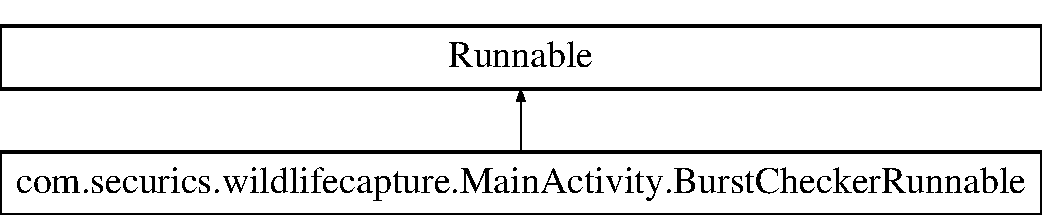
\includegraphics[height=2.000000cm]{classcom_1_1securics_1_1wildlifecapture_1_1_main_activity_1_1_burst_checker_runnable}
\end{center}
\end{figure}
\subsection*{Public Member Functions}
\begin{DoxyCompactItemize}
\item 
void {\bf run} ()
\end{DoxyCompactItemize}


\subsection{Detailed Description}


Definition at line 2595 of file Main\+Activity.\+java.



\subsection{Member Function Documentation}
\index{com\+::securics\+::wildlifecapture\+::\+Main\+Activity\+::\+Burst\+Checker\+Runnable@{com\+::securics\+::wildlifecapture\+::\+Main\+Activity\+::\+Burst\+Checker\+Runnable}!run@{run}}
\index{run@{run}!com\+::securics\+::wildlifecapture\+::\+Main\+Activity\+::\+Burst\+Checker\+Runnable@{com\+::securics\+::wildlifecapture\+::\+Main\+Activity\+::\+Burst\+Checker\+Runnable}}
\subsubsection[{run}]{\setlength{\rightskip}{0pt plus 5cm}void com.\+securics.\+wildlifecapture.\+Main\+Activity.\+Burst\+Checker\+Runnable.\+run (
\begin{DoxyParamCaption}
{}
\end{DoxyParamCaption}
)}\label{classcom_1_1securics_1_1wildlifecapture_1_1_main_activity_1_1_burst_checker_runnable_a974602d992f2a270d97af0127bd229de}


Definition at line 2599 of file Main\+Activity.\+java.



References com.\+securics.\+wildlifecapture.\+Main\+Activity.\+capture\+Burst(), com.\+securics.\+wildlifecapture.\+Main\+Activity.\+D\+E\+A\+T\+H, and com.\+securics.\+wildlifecapture.\+Main\+Activity.\+will\+Do\+Camera\+Burst.



The documentation for this class was generated from the following file\+:\begin{DoxyCompactItemize}
\item 
src/com/securics/wildlifecapture/{\bf Main\+Activity.\+java}\end{DoxyCompactItemize}

\section{com.\+securics.\+wildlifecapture.\+Main\+Activity.\+Burst\+Runnable Class Reference}
\label{classcom_1_1securics_1_1wildlifecapture_1_1_main_activity_1_1_burst_runnable}\index{com.\+securics.\+wildlifecapture.\+Main\+Activity.\+Burst\+Runnable@{com.\+securics.\+wildlifecapture.\+Main\+Activity.\+Burst\+Runnable}}
Inheritance diagram for com.\+securics.\+wildlifecapture.\+Main\+Activity.\+Burst\+Runnable\+:\begin{figure}[H]
\begin{center}
\leavevmode
\includegraphics[height=2.000000cm]{classcom_1_1securics_1_1wildlifecapture_1_1_main_activity_1_1_burst_runnable}
\end{center}
\end{figure}
\subsection*{Public Member Functions}
\begin{DoxyCompactItemize}
\item 
void {\bf run} ()
\end{DoxyCompactItemize}


\subsection{Detailed Description}
This is the main running part of the thread. 

Definition at line 2484 of file Main\+Activity.\+java.



\subsection{Member Function Documentation}
\index{com\+::securics\+::wildlifecapture\+::\+Main\+Activity\+::\+Burst\+Runnable@{com\+::securics\+::wildlifecapture\+::\+Main\+Activity\+::\+Burst\+Runnable}!run@{run}}
\index{run@{run}!com\+::securics\+::wildlifecapture\+::\+Main\+Activity\+::\+Burst\+Runnable@{com\+::securics\+::wildlifecapture\+::\+Main\+Activity\+::\+Burst\+Runnable}}
\subsubsection[{run}]{\setlength{\rightskip}{0pt plus 5cm}void com.\+securics.\+wildlifecapture.\+Main\+Activity.\+Burst\+Runnable.\+run (
\begin{DoxyParamCaption}
{}
\end{DoxyParamCaption}
)}\label{classcom_1_1securics_1_1wildlifecapture_1_1_main_activity_1_1_burst_runnable_aa7468198b80d156ac6540547993b9e9a}


Definition at line 2486 of file Main\+Activity.\+java.



References com.\+securics.\+wildlifecapture.\+Main\+Activity.\+burst\+Can\+Run, com.\+securics.\+wildlifecapture.\+Main\+Activity.\+burst\+Is\+Busy, com.\+securics.\+wildlifecapture.\+Main\+Activity.\+burst\+Num, com.\+securics.\+wildlifecapture.\+Main\+Activity.\+cam, com.\+securics.\+wildlifecapture.\+Main\+Activity.\+camera\+Lock, com.\+securics.\+wildlifecapture.\+Main\+Activity.\+D\+E\+A\+T\+H, com.\+securics.\+wildlifecapture.\+Main\+Activity.\+debug\+Mode, com.\+securics.\+wildlifecapture.\+Main\+Activity.\+m\+Debug, com.\+securics.\+wildlifecapture.\+Main\+Activity.\+Pic\+Callback, and com.\+securics.\+wildlifecapture.\+Main\+Activity.\+T\+A\+G.



The documentation for this class was generated from the following file\+:\begin{DoxyCompactItemize}
\item 
src/com/securics/wildlifecapture/{\bf Main\+Activity.\+java}\end{DoxyCompactItemize}

\section{com.\+securics.\+wildlifecapture.\+Camera\+Preference Class Reference}
\label{classcom_1_1securics_1_1wildlifecapture_1_1_camera_preference}\index{com.\+securics.\+wildlifecapture.\+Camera\+Preference@{com.\+securics.\+wildlifecapture.\+Camera\+Preference}}
Inheritance diagram for com.\+securics.\+wildlifecapture.\+Camera\+Preference\+:\begin{figure}[H]
\begin{center}
\leavevmode
\includegraphics[height=2.000000cm]{classcom_1_1securics_1_1wildlifecapture_1_1_camera_preference}
\end{center}
\end{figure}
\subsection*{Classes}
\begin{DoxyCompactItemize}
\item 
class {\bf My\+List}
\end{DoxyCompactItemize}
\subsection*{Public Member Functions}
\begin{DoxyCompactItemize}
\item 
{\bf Camera\+Preference} (Context context, Attribute\+Set attrs)
\end{DoxyCompactItemize}
\subsection*{Protected Member Functions}
\begin{DoxyCompactItemize}
\item 
void {\bf on\+Bind\+View} (View view)
\end{DoxyCompactItemize}
\subsection*{Private Member Functions}
\begin{DoxyCompactItemize}
\item 
void {\bf add\+My\+List} (Array\+List$<$ {\bf My\+List} $>$ lst)
\end{DoxyCompactItemize}


\subsection{Detailed Description}


Definition at line 15 of file Camera\+Preference.\+java.



\subsection{Constructor \& Destructor Documentation}
\index{com\+::securics\+::wildlifecapture\+::\+Camera\+Preference@{com\+::securics\+::wildlifecapture\+::\+Camera\+Preference}!Camera\+Preference@{Camera\+Preference}}
\index{Camera\+Preference@{Camera\+Preference}!com\+::securics\+::wildlifecapture\+::\+Camera\+Preference@{com\+::securics\+::wildlifecapture\+::\+Camera\+Preference}}
\subsubsection[{Camera\+Preference}]{\setlength{\rightskip}{0pt plus 5cm}com.\+securics.\+wildlifecapture.\+Camera\+Preference.\+Camera\+Preference (
\begin{DoxyParamCaption}
\item[{Context}]{context, }
\item[{Attribute\+Set}]{attrs}
\end{DoxyParamCaption}
)}\label{classcom_1_1securics_1_1wildlifecapture_1_1_camera_preference_a8d278f26779775355fffa614625d2547}
Sets class context, attrs using context and attrs. Creates and insert values in the\+List 
\begin{DoxyParams}{Parameters}
{\em context} & \\
\hline
{\em attrs} & \\
\hline
\end{DoxyParams}


Definition at line 27 of file Camera\+Preference.\+java.



\subsection{Member Function Documentation}
\index{com\+::securics\+::wildlifecapture\+::\+Camera\+Preference@{com\+::securics\+::wildlifecapture\+::\+Camera\+Preference}!add\+My\+List@{add\+My\+List}}
\index{add\+My\+List@{add\+My\+List}!com\+::securics\+::wildlifecapture\+::\+Camera\+Preference@{com\+::securics\+::wildlifecapture\+::\+Camera\+Preference}}
\subsubsection[{add\+My\+List}]{\setlength{\rightskip}{0pt plus 5cm}void com.\+securics.\+wildlifecapture.\+Camera\+Preference.\+add\+My\+List (
\begin{DoxyParamCaption}
\item[{Array\+List$<$ {\bf My\+List} $>$}]{lst}
\end{DoxyParamCaption}
)\hspace{0.3cm}{\ttfamily [private]}}\label{classcom_1_1securics_1_1wildlifecapture_1_1_camera_preference_aa0b8436a5ba6599a639e5dbec6cd8996}
Add te\+List to \doxyref{My\+List}{p.}{classcom_1_1securics_1_1wildlifecapture_1_1_camera_preference_1_1_my_list} 
\begin{DoxyParams}{Parameters}
{\em lst} & \\
\hline
\end{DoxyParams}


Definition at line 57 of file Camera\+Preference.\+java.



Referenced by com.\+securics.\+wildlifecapture.\+Camera\+Preference.\+on\+Bind\+View().

\index{com\+::securics\+::wildlifecapture\+::\+Camera\+Preference@{com\+::securics\+::wildlifecapture\+::\+Camera\+Preference}!on\+Bind\+View@{on\+Bind\+View}}
\index{on\+Bind\+View@{on\+Bind\+View}!com\+::securics\+::wildlifecapture\+::\+Camera\+Preference@{com\+::securics\+::wildlifecapture\+::\+Camera\+Preference}}
\subsubsection[{on\+Bind\+View}]{\setlength{\rightskip}{0pt plus 5cm}void com.\+securics.\+wildlifecapture.\+Camera\+Preference.\+on\+Bind\+View (
\begin{DoxyParamCaption}
\item[{View}]{view}
\end{DoxyParamCaption}
)\hspace{0.3cm}{\ttfamily [protected]}}\label{classcom_1_1securics_1_1wildlifecapture_1_1_camera_preference_a3fd6d1473b3089ee5ab4eef09c922980}
Calls add\+My\+List to ad the\+List to \doxyref{My\+List}{p.}{classcom_1_1securics_1_1wildlifecapture_1_1_camera_preference_1_1_my_list} 

Definition at line 47 of file Camera\+Preference.\+java.



References com.\+securics.\+wildlifecapture.\+Camera\+Preference.\+add\+My\+List().



The documentation for this class was generated from the following file\+:\begin{DoxyCompactItemize}
\item 
src/com/securics/wildlifecapture/{\bf Camera\+Preference.\+java}\end{DoxyCompactItemize}

\section{com.\+securics.\+wildlifecapture.\+Camera\+Preview Class Reference}
\label{classcom_1_1securics_1_1wildlifecapture_1_1_camera_preview}\index{com.\+securics.\+wildlifecapture.\+Camera\+Preview@{com.\+securics.\+wildlifecapture.\+Camera\+Preview}}
Inheritance diagram for com.\+securics.\+wildlifecapture.\+Camera\+Preview\+:\begin{figure}[H]
\begin{center}
\leavevmode
\includegraphics[height=2.000000cm]{classcom_1_1securics_1_1wildlifecapture_1_1_camera_preview}
\end{center}
\end{figure}
\subsection*{Public Member Functions}
\begin{DoxyCompactItemize}
\item 
{\bf Camera\+Preview} (Context context, Camera {\bf cam})
\item 
void {\bf surface\+Created} (Surface\+Holder holder)
\item 
void {\bf surface\+Changed} (Surface\+Holder holder, int format, int width, int height)
\item 
void {\bf surface\+Destroyed} (Surface\+Holder holder)
\end{DoxyCompactItemize}
\subsection*{Public Attributes}
\begin{DoxyCompactItemize}
\item 
Camera {\bf cam}
\end{DoxyCompactItemize}
\subsection*{Private Member Functions}
\begin{DoxyCompactItemize}
\item 
void {\bf init\+Camera} ()
\end{DoxyCompactItemize}
\subsection*{Private Attributes}
\begin{DoxyCompactItemize}
\item 
Surface\+Holder {\bf s\+Holder}
\end{DoxyCompactItemize}
\subsection*{Static Private Attributes}
\begin{DoxyCompactItemize}
\item 
static final String {\bf T\+A\+G} = \char`\"{}Camera\+Preview\char`\"{}
\end{DoxyCompactItemize}


\subsection{Detailed Description}


Definition at line 15 of file Camera\+Preview.\+java.



\subsection{Constructor \& Destructor Documentation}
\index{com\+::securics\+::wildlifecapture\+::\+Camera\+Preview@{com\+::securics\+::wildlifecapture\+::\+Camera\+Preview}!Camera\+Preview@{Camera\+Preview}}
\index{Camera\+Preview@{Camera\+Preview}!com\+::securics\+::wildlifecapture\+::\+Camera\+Preview@{com\+::securics\+::wildlifecapture\+::\+Camera\+Preview}}
\subsubsection[{Camera\+Preview}]{\setlength{\rightskip}{0pt plus 5cm}com.\+securics.\+wildlifecapture.\+Camera\+Preview.\+Camera\+Preview (
\begin{DoxyParamCaption}
\item[{Context}]{context, }
\item[{Camera}]{cam}
\end{DoxyParamCaption}
)}\label{classcom_1_1securics_1_1wildlifecapture_1_1_camera_preview_a98ff2a8512cd75a9d7981a962d396814}
Call init\+Camera to set camera 
\begin{DoxyParams}{Parameters}
{\em context} & \\
\hline
{\em cam} & \\
\hline
\end{DoxyParams}


Definition at line 27 of file Camera\+Preview.\+java.



References com.\+securics.\+wildlifecapture.\+Camera\+Preview.\+cam, com.\+securics.\+wildlifecapture.\+Main\+Activity.\+debug\+Mode, com.\+securics.\+wildlifecapture.\+Camera\+Preview.\+init\+Camera(), com.\+securics.\+wildlifecapture.\+Camera\+Preview.\+s\+Holder, and com.\+securics.\+wildlifecapture.\+Camera\+Preview.\+T\+A\+G.



\subsection{Member Function Documentation}
\index{com\+::securics\+::wildlifecapture\+::\+Camera\+Preview@{com\+::securics\+::wildlifecapture\+::\+Camera\+Preview}!init\+Camera@{init\+Camera}}
\index{init\+Camera@{init\+Camera}!com\+::securics\+::wildlifecapture\+::\+Camera\+Preview@{com\+::securics\+::wildlifecapture\+::\+Camera\+Preview}}
\subsubsection[{init\+Camera}]{\setlength{\rightskip}{0pt plus 5cm}void com.\+securics.\+wildlifecapture.\+Camera\+Preview.\+init\+Camera (
\begin{DoxyParamCaption}
{}
\end{DoxyParamCaption}
)\hspace{0.3cm}{\ttfamily [private]}}\label{classcom_1_1securics_1_1wildlifecapture_1_1_camera_preview_a9ae15f792a1663007353246d533c2da9}
Set camera parameters to preferred settings 

Definition at line 42 of file Camera\+Preview.\+java.



References com.\+securics.\+wildlifecapture.\+Main\+Activity.\+debug\+Mode, and com.\+securics.\+wildlifecapture.\+Camera\+Preview.\+T\+A\+G.



Referenced by com.\+securics.\+wildlifecapture.\+Camera\+Preview.\+Camera\+Preview().

\index{com\+::securics\+::wildlifecapture\+::\+Camera\+Preview@{com\+::securics\+::wildlifecapture\+::\+Camera\+Preview}!surface\+Changed@{surface\+Changed}}
\index{surface\+Changed@{surface\+Changed}!com\+::securics\+::wildlifecapture\+::\+Camera\+Preview@{com\+::securics\+::wildlifecapture\+::\+Camera\+Preview}}
\subsubsection[{surface\+Changed}]{\setlength{\rightskip}{0pt plus 5cm}void com.\+securics.\+wildlifecapture.\+Camera\+Preview.\+surface\+Changed (
\begin{DoxyParamCaption}
\item[{Surface\+Holder}]{holder, }
\item[{int}]{format, }
\item[{int}]{width, }
\item[{int}]{height}
\end{DoxyParamCaption}
)}\label{classcom_1_1securics_1_1wildlifecapture_1_1_camera_preview_ab804fbe7dc204b3f87897720610779ac}
previews if camera is on 

Definition at line 98 of file Camera\+Preview.\+java.



References com.\+securics.\+wildlifecapture.\+Camera\+Preview.\+cam, and com.\+securics.\+wildlifecapture.\+Main\+Activity.\+debug\+Mode.

\index{com\+::securics\+::wildlifecapture\+::\+Camera\+Preview@{com\+::securics\+::wildlifecapture\+::\+Camera\+Preview}!surface\+Created@{surface\+Created}}
\index{surface\+Created@{surface\+Created}!com\+::securics\+::wildlifecapture\+::\+Camera\+Preview@{com\+::securics\+::wildlifecapture\+::\+Camera\+Preview}}
\subsubsection[{surface\+Created}]{\setlength{\rightskip}{0pt plus 5cm}void com.\+securics.\+wildlifecapture.\+Camera\+Preview.\+surface\+Created (
\begin{DoxyParamCaption}
\item[{Surface\+Holder}]{holder}
\end{DoxyParamCaption}
)}\label{classcom_1_1securics_1_1wildlifecapture_1_1_camera_preview_aac6d23452b929eade3d3550b230b2d7e}
previews displau of camera is on 

Definition at line 82 of file Camera\+Preview.\+java.



References com.\+securics.\+wildlifecapture.\+Camera\+Preview.\+cam, com.\+securics.\+wildlifecapture.\+Main\+Activity.\+debug\+Mode, com.\+securics.\+wildlifecapture.\+Camera\+Preview.\+s\+Holder, and com.\+securics.\+wildlifecapture.\+Camera\+Preview.\+T\+A\+G.

\index{com\+::securics\+::wildlifecapture\+::\+Camera\+Preview@{com\+::securics\+::wildlifecapture\+::\+Camera\+Preview}!surface\+Destroyed@{surface\+Destroyed}}
\index{surface\+Destroyed@{surface\+Destroyed}!com\+::securics\+::wildlifecapture\+::\+Camera\+Preview@{com\+::securics\+::wildlifecapture\+::\+Camera\+Preview}}
\subsubsection[{surface\+Destroyed}]{\setlength{\rightskip}{0pt plus 5cm}void com.\+securics.\+wildlifecapture.\+Camera\+Preview.\+surface\+Destroyed (
\begin{DoxyParamCaption}
\item[{Surface\+Holder}]{holder}
\end{DoxyParamCaption}
)}\label{classcom_1_1securics_1_1wildlifecapture_1_1_camera_preview_a515e4c00aef971f61431ba02c90d3ebf}
closes camera 

Definition at line 114 of file Camera\+Preview.\+java.



References com.\+securics.\+wildlifecapture.\+Camera\+Preview.\+cam, and com.\+securics.\+wildlifecapture.\+Main\+Activity.\+debug\+Mode.



\subsection{Member Data Documentation}
\index{com\+::securics\+::wildlifecapture\+::\+Camera\+Preview@{com\+::securics\+::wildlifecapture\+::\+Camera\+Preview}!cam@{cam}}
\index{cam@{cam}!com\+::securics\+::wildlifecapture\+::\+Camera\+Preview@{com\+::securics\+::wildlifecapture\+::\+Camera\+Preview}}
\subsubsection[{cam}]{\setlength{\rightskip}{0pt plus 5cm}Camera com.\+securics.\+wildlifecapture.\+Camera\+Preview.\+cam}\label{classcom_1_1securics_1_1wildlifecapture_1_1_camera_preview_a97c474f61cd67209524fa379894ce528}


Definition at line 19 of file Camera\+Preview.\+java.



Referenced by com.\+securics.\+wildlifecapture.\+Camera\+Preview.\+Camera\+Preview(), com.\+securics.\+wildlifecapture.\+Camera\+Preview.\+surface\+Changed(), com.\+securics.\+wildlifecapture.\+Camera\+Preview.\+surface\+Created(), and com.\+securics.\+wildlifecapture.\+Camera\+Preview.\+surface\+Destroyed().

\index{com\+::securics\+::wildlifecapture\+::\+Camera\+Preview@{com\+::securics\+::wildlifecapture\+::\+Camera\+Preview}!s\+Holder@{s\+Holder}}
\index{s\+Holder@{s\+Holder}!com\+::securics\+::wildlifecapture\+::\+Camera\+Preview@{com\+::securics\+::wildlifecapture\+::\+Camera\+Preview}}
\subsubsection[{s\+Holder}]{\setlength{\rightskip}{0pt plus 5cm}Surface\+Holder com.\+securics.\+wildlifecapture.\+Camera\+Preview.\+s\+Holder\hspace{0.3cm}{\ttfamily [private]}}\label{classcom_1_1securics_1_1wildlifecapture_1_1_camera_preview_af07f87b9a8ff4d898182999976bdd0d5}


Definition at line 20 of file Camera\+Preview.\+java.



Referenced by com.\+securics.\+wildlifecapture.\+Camera\+Preview.\+Camera\+Preview(), and com.\+securics.\+wildlifecapture.\+Camera\+Preview.\+surface\+Created().

\index{com\+::securics\+::wildlifecapture\+::\+Camera\+Preview@{com\+::securics\+::wildlifecapture\+::\+Camera\+Preview}!T\+A\+G@{T\+A\+G}}
\index{T\+A\+G@{T\+A\+G}!com\+::securics\+::wildlifecapture\+::\+Camera\+Preview@{com\+::securics\+::wildlifecapture\+::\+Camera\+Preview}}
\subsubsection[{T\+A\+G}]{\setlength{\rightskip}{0pt plus 5cm}final String com.\+securics.\+wildlifecapture.\+Camera\+Preview.\+T\+A\+G = \char`\"{}Camera\+Preview\char`\"{}\hspace{0.3cm}{\ttfamily [static]}, {\ttfamily [private]}}\label{classcom_1_1securics_1_1wildlifecapture_1_1_camera_preview_ada374cd3791b887dbbfc1ee7de9faacc}


Definition at line 16 of file Camera\+Preview.\+java.



Referenced by com.\+securics.\+wildlifecapture.\+Camera\+Preview.\+Camera\+Preview(), com.\+securics.\+wildlifecapture.\+Camera\+Preview.\+init\+Camera(), and com.\+securics.\+wildlifecapture.\+Camera\+Preview.\+surface\+Created().



The documentation for this class was generated from the following file\+:\begin{DoxyCompactItemize}
\item 
src/com/securics/wildlifecapture/{\bf Camera\+Preview.\+java}\end{DoxyCompactItemize}

\section{com.\+securics.\+wildlifecapture.\+Change\+Resolution\+Activity Class Reference}
\label{classcom_1_1securics_1_1wildlifecapture_1_1_change_resolution_activity}\index{com.\+securics.\+wildlifecapture.\+Change\+Resolution\+Activity@{com.\+securics.\+wildlifecapture.\+Change\+Resolution\+Activity}}
Inheritance diagram for com.\+securics.\+wildlifecapture.\+Change\+Resolution\+Activity\+:\begin{figure}[H]
\begin{center}
\leavevmode
\includegraphics[height=2.000000cm]{classcom_1_1securics_1_1wildlifecapture_1_1_change_resolution_activity}
\end{center}
\end{figure}
\subsection*{Public Member Functions}
\begin{DoxyCompactItemize}
\item 
void {\bf get\+Size\+Data} ()
\item 
void {\bf size\+To\+String} ()
\item 
void {\bf set\+List\+View} ()
\item 
boolean {\bf on\+Create\+Options\+Menu} (Menu menu)
\item 
void {\bf on\+List\+Item\+Click} (List\+View tmp, View v, int pos, long id)
\end{DoxyCompactItemize}
\subsection*{Protected Member Functions}
\begin{DoxyCompactItemize}
\item 
void {\bf on\+Create} (Bundle saved\+Instance\+State)
\item 
void {\bf on\+Resume} ()
\end{DoxyCompactItemize}
\subsection*{Private Member Functions}
\begin{DoxyCompactItemize}
\item 
Camera {\bf get\+Camera\+Instance} ()
\end{DoxyCompactItemize}
\subsection*{Private Attributes}
\begin{DoxyCompactItemize}
\item 
List\+View {\bf internal\+View}
\item 
Camera {\bf cam\+Copy}
\item 
Size {\bf pic\+Size}
\item 
List$<$ Size $>$ {\bf size\+List}
\item 
String[$\,$] {\bf size\+Names}
\end{DoxyCompactItemize}


\subsection{Detailed Description}


Definition at line 16 of file Change\+Resolution\+Activity.\+java.



\subsection{Member Function Documentation}
\index{com\+::securics\+::wildlifecapture\+::\+Change\+Resolution\+Activity@{com\+::securics\+::wildlifecapture\+::\+Change\+Resolution\+Activity}!get\+Camera\+Instance@{get\+Camera\+Instance}}
\index{get\+Camera\+Instance@{get\+Camera\+Instance}!com\+::securics\+::wildlifecapture\+::\+Change\+Resolution\+Activity@{com\+::securics\+::wildlifecapture\+::\+Change\+Resolution\+Activity}}
\subsubsection[{get\+Camera\+Instance}]{\setlength{\rightskip}{0pt plus 5cm}Camera com.\+securics.\+wildlifecapture.\+Change\+Resolution\+Activity.\+get\+Camera\+Instance (
\begin{DoxyParamCaption}
{}
\end{DoxyParamCaption}
)\hspace{0.3cm}{\ttfamily [private]}}\label{classcom_1_1securics_1_1wildlifecapture_1_1_change_resolution_activity_a98b2bd95379921a8b75f94f836e0e60f}
Attempt to get a camera. 

Definition at line 135 of file Change\+Resolution\+Activity.\+java.



References com.\+securics.\+wildlifecapture.\+Main\+Activity.\+debug\+Mode.



Referenced by com.\+securics.\+wildlifecapture.\+Change\+Resolution\+Activity.\+on\+Resume().

\index{com\+::securics\+::wildlifecapture\+::\+Change\+Resolution\+Activity@{com\+::securics\+::wildlifecapture\+::\+Change\+Resolution\+Activity}!get\+Size\+Data@{get\+Size\+Data}}
\index{get\+Size\+Data@{get\+Size\+Data}!com\+::securics\+::wildlifecapture\+::\+Change\+Resolution\+Activity@{com\+::securics\+::wildlifecapture\+::\+Change\+Resolution\+Activity}}
\subsubsection[{get\+Size\+Data}]{\setlength{\rightskip}{0pt plus 5cm}void com.\+securics.\+wildlifecapture.\+Change\+Resolution\+Activity.\+get\+Size\+Data (
\begin{DoxyParamCaption}
{}
\end{DoxyParamCaption}
)}\label{classcom_1_1securics_1_1wildlifecapture_1_1_change_resolution_activity_aef0e2e7375dd5b11be1e83cfccd2c301}
This should probably be able to potentially maybe get the size\+List from the non-\/static copy of the static camera contained in \doxyref{Main\+Activity}{p.}{classcom_1_1securics_1_1wildlifecapture_1_1_main_activity}. 

Definition at line 28 of file Change\+Resolution\+Activity.\+java.



References com.\+securics.\+wildlifecapture.\+Change\+Resolution\+Activity.\+size\+List.



Referenced by com.\+securics.\+wildlifecapture.\+Change\+Resolution\+Activity.\+on\+Resume().

\index{com\+::securics\+::wildlifecapture\+::\+Change\+Resolution\+Activity@{com\+::securics\+::wildlifecapture\+::\+Change\+Resolution\+Activity}!on\+Create@{on\+Create}}
\index{on\+Create@{on\+Create}!com\+::securics\+::wildlifecapture\+::\+Change\+Resolution\+Activity@{com\+::securics\+::wildlifecapture\+::\+Change\+Resolution\+Activity}}
\subsubsection[{on\+Create}]{\setlength{\rightskip}{0pt plus 5cm}void com.\+securics.\+wildlifecapture.\+Change\+Resolution\+Activity.\+on\+Create (
\begin{DoxyParamCaption}
\item[{Bundle}]{saved\+Instance\+State}
\end{DoxyParamCaption}
)\hspace{0.3cm}{\ttfamily [protected]}}\label{classcom_1_1securics_1_1wildlifecapture_1_1_change_resolution_activity_ad0fe1988bd214444cce7aeb4a8af91c4}
set layout 

Definition at line 75 of file Change\+Resolution\+Activity.\+java.

\index{com\+::securics\+::wildlifecapture\+::\+Change\+Resolution\+Activity@{com\+::securics\+::wildlifecapture\+::\+Change\+Resolution\+Activity}!on\+Create\+Options\+Menu@{on\+Create\+Options\+Menu}}
\index{on\+Create\+Options\+Menu@{on\+Create\+Options\+Menu}!com\+::securics\+::wildlifecapture\+::\+Change\+Resolution\+Activity@{com\+::securics\+::wildlifecapture\+::\+Change\+Resolution\+Activity}}
\subsubsection[{on\+Create\+Options\+Menu}]{\setlength{\rightskip}{0pt plus 5cm}boolean com.\+securics.\+wildlifecapture.\+Change\+Resolution\+Activity.\+on\+Create\+Options\+Menu (
\begin{DoxyParamCaption}
\item[{Menu}]{menu}
\end{DoxyParamCaption}
)}\label{classcom_1_1securics_1_1wildlifecapture_1_1_change_resolution_activity_a9257daf73e6172dfbe622d485c8d9053}
Create an option menu Inflate the menu; this adds items to the action bar if it is present. 

Definition at line 109 of file Change\+Resolution\+Activity.\+java.

\index{com\+::securics\+::wildlifecapture\+::\+Change\+Resolution\+Activity@{com\+::securics\+::wildlifecapture\+::\+Change\+Resolution\+Activity}!on\+List\+Item\+Click@{on\+List\+Item\+Click}}
\index{on\+List\+Item\+Click@{on\+List\+Item\+Click}!com\+::securics\+::wildlifecapture\+::\+Change\+Resolution\+Activity@{com\+::securics\+::wildlifecapture\+::\+Change\+Resolution\+Activity}}
\subsubsection[{on\+List\+Item\+Click}]{\setlength{\rightskip}{0pt plus 5cm}void com.\+securics.\+wildlifecapture.\+Change\+Resolution\+Activity.\+on\+List\+Item\+Click (
\begin{DoxyParamCaption}
\item[{List\+View}]{tmp, }
\item[{View}]{v, }
\item[{int}]{pos, }
\item[{long}]{id}
\end{DoxyParamCaption}
)}\label{classcom_1_1securics_1_1wildlifecapture_1_1_change_resolution_activity_a513eca395f902994466650ac38a07b85}
Set resolution on \doxyref{Main\+Activity}{p.}{classcom_1_1securics_1_1wildlifecapture_1_1_main_activity} 

Definition at line 118 of file Change\+Resolution\+Activity.\+java.



References com.\+securics.\+wildlifecapture.\+Change\+Resolution\+Activity.\+cam\+Copy, and com.\+securics.\+wildlifecapture.\+Change\+Resolution\+Activity.\+size\+Names.

\index{com\+::securics\+::wildlifecapture\+::\+Change\+Resolution\+Activity@{com\+::securics\+::wildlifecapture\+::\+Change\+Resolution\+Activity}!on\+Resume@{on\+Resume}}
\index{on\+Resume@{on\+Resume}!com\+::securics\+::wildlifecapture\+::\+Change\+Resolution\+Activity@{com\+::securics\+::wildlifecapture\+::\+Change\+Resolution\+Activity}}
\subsubsection[{on\+Resume}]{\setlength{\rightskip}{0pt plus 5cm}void com.\+securics.\+wildlifecapture.\+Change\+Resolution\+Activity.\+on\+Resume (
\begin{DoxyParamCaption}
{}
\end{DoxyParamCaption}
)\hspace{0.3cm}{\ttfamily [protected]}}\label{classcom_1_1securics_1_1wildlifecapture_1_1_change_resolution_activity_a08c2b11c761468de4b0adfb1fe19451c}
get instance of camera 

Definition at line 85 of file Change\+Resolution\+Activity.\+java.



References com.\+securics.\+wildlifecapture.\+Change\+Resolution\+Activity.\+cam\+Copy, com.\+securics.\+wildlifecapture.\+Change\+Resolution\+Activity.\+get\+Camera\+Instance(), com.\+securics.\+wildlifecapture.\+Change\+Resolution\+Activity.\+get\+Size\+Data(), com.\+securics.\+wildlifecapture.\+Change\+Resolution\+Activity.\+internal\+View, com.\+securics.\+wildlifecapture.\+Change\+Resolution\+Activity.\+set\+List\+View(), and com.\+securics.\+wildlifecapture.\+Change\+Resolution\+Activity.\+size\+To\+String().

\index{com\+::securics\+::wildlifecapture\+::\+Change\+Resolution\+Activity@{com\+::securics\+::wildlifecapture\+::\+Change\+Resolution\+Activity}!set\+List\+View@{set\+List\+View}}
\index{set\+List\+View@{set\+List\+View}!com\+::securics\+::wildlifecapture\+::\+Change\+Resolution\+Activity@{com\+::securics\+::wildlifecapture\+::\+Change\+Resolution\+Activity}}
\subsubsection[{set\+List\+View}]{\setlength{\rightskip}{0pt plus 5cm}void com.\+securics.\+wildlifecapture.\+Change\+Resolution\+Activity.\+set\+List\+View (
\begin{DoxyParamCaption}
{}
\end{DoxyParamCaption}
)}\label{classcom_1_1securics_1_1wildlifecapture_1_1_change_resolution_activity_a0b9caa29636ab330db88a52a33505420}
set list adapter Set up the array adapter. 

Definition at line 64 of file Change\+Resolution\+Activity.\+java.



References com.\+securics.\+wildlifecapture.\+Change\+Resolution\+Activity.\+size\+Names.



Referenced by com.\+securics.\+wildlifecapture.\+Change\+Resolution\+Activity.\+on\+Resume().

\index{com\+::securics\+::wildlifecapture\+::\+Change\+Resolution\+Activity@{com\+::securics\+::wildlifecapture\+::\+Change\+Resolution\+Activity}!size\+To\+String@{size\+To\+String}}
\index{size\+To\+String@{size\+To\+String}!com\+::securics\+::wildlifecapture\+::\+Change\+Resolution\+Activity@{com\+::securics\+::wildlifecapture\+::\+Change\+Resolution\+Activity}}
\subsubsection[{size\+To\+String}]{\setlength{\rightskip}{0pt plus 5cm}void com.\+securics.\+wildlifecapture.\+Change\+Resolution\+Activity.\+size\+To\+String (
\begin{DoxyParamCaption}
{}
\end{DoxyParamCaption}
)}\label{classcom_1_1securics_1_1wildlifecapture_1_1_change_resolution_activity_a021c5c14e5a3e03cb43f29d5fe112997}
Add all picture sizes to size\+Names array 

Definition at line 39 of file Change\+Resolution\+Activity.\+java.



References com.\+securics.\+wildlifecapture.\+Change\+Resolution\+Activity.\+size\+List, and com.\+securics.\+wildlifecapture.\+Change\+Resolution\+Activity.\+size\+Names.



Referenced by com.\+securics.\+wildlifecapture.\+Change\+Resolution\+Activity.\+on\+Resume().



\subsection{Member Data Documentation}
\index{com\+::securics\+::wildlifecapture\+::\+Change\+Resolution\+Activity@{com\+::securics\+::wildlifecapture\+::\+Change\+Resolution\+Activity}!cam\+Copy@{cam\+Copy}}
\index{cam\+Copy@{cam\+Copy}!com\+::securics\+::wildlifecapture\+::\+Change\+Resolution\+Activity@{com\+::securics\+::wildlifecapture\+::\+Change\+Resolution\+Activity}}
\subsubsection[{cam\+Copy}]{\setlength{\rightskip}{0pt plus 5cm}Camera com.\+securics.\+wildlifecapture.\+Change\+Resolution\+Activity.\+cam\+Copy\hspace{0.3cm}{\ttfamily [private]}}\label{classcom_1_1securics_1_1wildlifecapture_1_1_change_resolution_activity_a6b50fb23769ed5f2c15feaf5556b321a}


Definition at line 19 of file Change\+Resolution\+Activity.\+java.



Referenced by com.\+securics.\+wildlifecapture.\+Change\+Resolution\+Activity.\+on\+List\+Item\+Click(), and com.\+securics.\+wildlifecapture.\+Change\+Resolution\+Activity.\+on\+Resume().

\index{com\+::securics\+::wildlifecapture\+::\+Change\+Resolution\+Activity@{com\+::securics\+::wildlifecapture\+::\+Change\+Resolution\+Activity}!internal\+View@{internal\+View}}
\index{internal\+View@{internal\+View}!com\+::securics\+::wildlifecapture\+::\+Change\+Resolution\+Activity@{com\+::securics\+::wildlifecapture\+::\+Change\+Resolution\+Activity}}
\subsubsection[{internal\+View}]{\setlength{\rightskip}{0pt plus 5cm}List\+View com.\+securics.\+wildlifecapture.\+Change\+Resolution\+Activity.\+internal\+View\hspace{0.3cm}{\ttfamily [private]}}\label{classcom_1_1securics_1_1wildlifecapture_1_1_change_resolution_activity_a66e338edadd91789e8ec6f1d2e3ac988}


Definition at line 18 of file Change\+Resolution\+Activity.\+java.



Referenced by com.\+securics.\+wildlifecapture.\+Change\+Resolution\+Activity.\+on\+Resume().

\index{com\+::securics\+::wildlifecapture\+::\+Change\+Resolution\+Activity@{com\+::securics\+::wildlifecapture\+::\+Change\+Resolution\+Activity}!pic\+Size@{pic\+Size}}
\index{pic\+Size@{pic\+Size}!com\+::securics\+::wildlifecapture\+::\+Change\+Resolution\+Activity@{com\+::securics\+::wildlifecapture\+::\+Change\+Resolution\+Activity}}
\subsubsection[{pic\+Size}]{\setlength{\rightskip}{0pt plus 5cm}Size com.\+securics.\+wildlifecapture.\+Change\+Resolution\+Activity.\+pic\+Size\hspace{0.3cm}{\ttfamily [private]}}\label{classcom_1_1securics_1_1wildlifecapture_1_1_change_resolution_activity_aa177f6f8767814e1884e32694cd2b0e8}


Definition at line 20 of file Change\+Resolution\+Activity.\+java.

\index{com\+::securics\+::wildlifecapture\+::\+Change\+Resolution\+Activity@{com\+::securics\+::wildlifecapture\+::\+Change\+Resolution\+Activity}!size\+List@{size\+List}}
\index{size\+List@{size\+List}!com\+::securics\+::wildlifecapture\+::\+Change\+Resolution\+Activity@{com\+::securics\+::wildlifecapture\+::\+Change\+Resolution\+Activity}}
\subsubsection[{size\+List}]{\setlength{\rightskip}{0pt plus 5cm}List$<$Size$>$ com.\+securics.\+wildlifecapture.\+Change\+Resolution\+Activity.\+size\+List\hspace{0.3cm}{\ttfamily [private]}}\label{classcom_1_1securics_1_1wildlifecapture_1_1_change_resolution_activity_ae85857326d2d3e3a6e3a99add2918112}


Definition at line 21 of file Change\+Resolution\+Activity.\+java.



Referenced by com.\+securics.\+wildlifecapture.\+Change\+Resolution\+Activity.\+get\+Size\+Data(), and com.\+securics.\+wildlifecapture.\+Change\+Resolution\+Activity.\+size\+To\+String().

\index{com\+::securics\+::wildlifecapture\+::\+Change\+Resolution\+Activity@{com\+::securics\+::wildlifecapture\+::\+Change\+Resolution\+Activity}!size\+Names@{size\+Names}}
\index{size\+Names@{size\+Names}!com\+::securics\+::wildlifecapture\+::\+Change\+Resolution\+Activity@{com\+::securics\+::wildlifecapture\+::\+Change\+Resolution\+Activity}}
\subsubsection[{size\+Names}]{\setlength{\rightskip}{0pt plus 5cm}String [$\,$] com.\+securics.\+wildlifecapture.\+Change\+Resolution\+Activity.\+size\+Names\hspace{0.3cm}{\ttfamily [private]}}\label{classcom_1_1securics_1_1wildlifecapture_1_1_change_resolution_activity_a565b5e88750a511709118a7c2eb2ece4}


Definition at line 22 of file Change\+Resolution\+Activity.\+java.



Referenced by com.\+securics.\+wildlifecapture.\+Change\+Resolution\+Activity.\+on\+List\+Item\+Click(), com.\+securics.\+wildlifecapture.\+Change\+Resolution\+Activity.\+set\+List\+View(), and com.\+securics.\+wildlifecapture.\+Change\+Resolution\+Activity.\+size\+To\+String().



The documentation for this class was generated from the following file\+:\begin{DoxyCompactItemize}
\item 
src/com/securics/wildlifecapture/{\bf Change\+Resolution\+Activity.\+java}\end{DoxyCompactItemize}

\section{com.\+securics.\+wildlifecapture.\+Documentation Class Reference}
\label{classcom_1_1securics_1_1wildlifecapture_1_1_documentation}\index{com.\+securics.\+wildlifecapture.\+Documentation@{com.\+securics.\+wildlifecapture.\+Documentation}}
Inheritance diagram for com.\+securics.\+wildlifecapture.\+Documentation\+:\begin{figure}[H]
\begin{center}
\leavevmode
\includegraphics[height=2.000000cm]{classcom_1_1securics_1_1wildlifecapture_1_1_documentation}
\end{center}
\end{figure}
\subsection*{Public Member Functions}
\begin{DoxyCompactItemize}
\item 
boolean {\bf on\+Create\+Options\+Menu} (Menu menu)
\item 
boolean {\bf on\+Options\+Item\+Selected} (Menu\+Item item)
\end{DoxyCompactItemize}
\subsection*{Protected Member Functions}
\begin{DoxyCompactItemize}
\item 
void {\bf on\+Create} (Bundle saved\+Instance\+State)
\end{DoxyCompactItemize}


\subsection{Detailed Description}
This activity is an online documentation engine for the program. The way this activity displays documentation is via a package-\/integrated web page. It may be possible to eventually have a tabbed help interface that loads individual H\+T\+M\+L pages for every section, however that will not be implemented soon. 

Definition at line 19 of file Documentation.\+java.



\subsection{Member Function Documentation}
\index{com\+::securics\+::wildlifecapture\+::\+Documentation@{com\+::securics\+::wildlifecapture\+::\+Documentation}!on\+Create@{on\+Create}}
\index{on\+Create@{on\+Create}!com\+::securics\+::wildlifecapture\+::\+Documentation@{com\+::securics\+::wildlifecapture\+::\+Documentation}}
\subsubsection[{on\+Create}]{\setlength{\rightskip}{0pt plus 5cm}void com.\+securics.\+wildlifecapture.\+Documentation.\+on\+Create (
\begin{DoxyParamCaption}
\item[{Bundle}]{saved\+Instance\+State}
\end{DoxyParamCaption}
)\hspace{0.3cm}{\ttfamily [protected]}}\label{classcom_1_1securics_1_1wildlifecapture_1_1_documentation_af0e18fb5bd692dd994b8efa22af5b385}
Set activity layout and action bar Note\+: There should be a table of if statements regarding the tab names and which page to load.

Definition at line 31 of file Documentation.\+java.

\index{com\+::securics\+::wildlifecapture\+::\+Documentation@{com\+::securics\+::wildlifecapture\+::\+Documentation}!on\+Create\+Options\+Menu@{on\+Create\+Options\+Menu}}
\index{on\+Create\+Options\+Menu@{on\+Create\+Options\+Menu}!com\+::securics\+::wildlifecapture\+::\+Documentation@{com\+::securics\+::wildlifecapture\+::\+Documentation}}
\subsubsection[{on\+Create\+Options\+Menu}]{\setlength{\rightskip}{0pt plus 5cm}boolean com.\+securics.\+wildlifecapture.\+Documentation.\+on\+Create\+Options\+Menu (
\begin{DoxyParamCaption}
\item[{Menu}]{menu}
\end{DoxyParamCaption}
)}\label{classcom_1_1securics_1_1wildlifecapture_1_1_documentation_ab25a6dfdd7285c57a4fbb00e52b3b7b5}
Creates a menu 

Definition at line 125 of file Documentation.\+java.

\index{com\+::securics\+::wildlifecapture\+::\+Documentation@{com\+::securics\+::wildlifecapture\+::\+Documentation}!on\+Options\+Item\+Selected@{on\+Options\+Item\+Selected}}
\index{on\+Options\+Item\+Selected@{on\+Options\+Item\+Selected}!com\+::securics\+::wildlifecapture\+::\+Documentation@{com\+::securics\+::wildlifecapture\+::\+Documentation}}
\subsubsection[{on\+Options\+Item\+Selected}]{\setlength{\rightskip}{0pt plus 5cm}boolean com.\+securics.\+wildlifecapture.\+Documentation.\+on\+Options\+Item\+Selected (
\begin{DoxyParamCaption}
\item[{Menu\+Item}]{item}
\end{DoxyParamCaption}
)}\label{classcom_1_1securics_1_1wildlifecapture_1_1_documentation_afd33e6cc75dc22a1cc2add67cd87a12a}
Listener for on\+Create\+Options\+Menu 

Definition at line 135 of file Documentation.\+java.



The documentation for this class was generated from the following file\+:\begin{DoxyCompactItemize}
\item 
src/com/securics/wildlifecapture/{\bf Documentation.\+java}\end{DoxyCompactItemize}

\section{com.\+securics.\+wildlifecapture.\+General\+Settings Class Reference}
\label{classcom_1_1securics_1_1wildlifecapture_1_1_general_settings}\index{com.\+securics.\+wildlifecapture.\+General\+Settings@{com.\+securics.\+wildlifecapture.\+General\+Settings}}
Inheritance diagram for com.\+securics.\+wildlifecapture.\+General\+Settings\+:\begin{figure}[H]
\begin{center}
\leavevmode
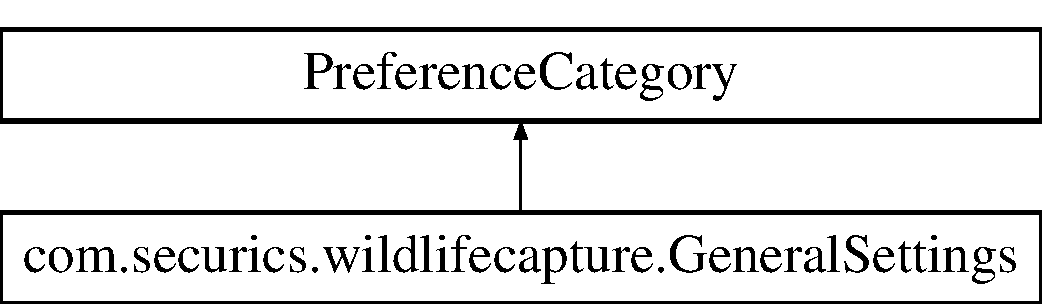
\includegraphics[height=2.000000cm]{classcom_1_1securics_1_1wildlifecapture_1_1_general_settings}
\end{center}
\end{figure}
\subsection*{Public Member Functions}
\begin{DoxyCompactItemize}
\item 
{\bf General\+Settings} (Context context, Attribute\+Set attrs)
\end{DoxyCompactItemize}
\subsection*{Protected Member Functions}
\begin{DoxyCompactItemize}
\item 
void {\bf on\+Bind\+View} (View view)
\end{DoxyCompactItemize}
\subsection*{Private Member Functions}
\begin{DoxyCompactItemize}
\item 
void {\bf load\+Params} ()
\end{DoxyCompactItemize}


\subsection{Detailed Description}


Definition at line 9 of file General\+Settings.\+java.



\subsection{Constructor \& Destructor Documentation}
\index{com\+::securics\+::wildlifecapture\+::\+General\+Settings@{com\+::securics\+::wildlifecapture\+::\+General\+Settings}!General\+Settings@{General\+Settings}}
\index{General\+Settings@{General\+Settings}!com\+::securics\+::wildlifecapture\+::\+General\+Settings@{com\+::securics\+::wildlifecapture\+::\+General\+Settings}}
\subsubsection[{General\+Settings}]{\setlength{\rightskip}{0pt plus 5cm}com.\+securics.\+wildlifecapture.\+General\+Settings.\+General\+Settings (
\begin{DoxyParamCaption}
\item[{Context}]{context, }
\item[{Attribute\+Set}]{attrs}
\end{DoxyParamCaption}
)}\label{classcom_1_1securics_1_1wildlifecapture_1_1_general_settings_a947ed82c58f96a484976d6fb96dd87db}
Depending on tittle from context, input the array from either generalstuff or general\+\_\+swindow 
\begin{DoxyParams}{Parameters}
{\em context} & \\
\hline
{\em attrs} & \\
\hline
\end{DoxyParams}


Definition at line 22 of file General\+Settings.\+java.



References com.\+securics.\+wildlifecapture.\+Main\+Activity.\+debug\+Mode.



\subsection{Member Function Documentation}
\index{com\+::securics\+::wildlifecapture\+::\+General\+Settings@{com\+::securics\+::wildlifecapture\+::\+General\+Settings}!load\+Params@{load\+Params}}
\index{load\+Params@{load\+Params}!com\+::securics\+::wildlifecapture\+::\+General\+Settings@{com\+::securics\+::wildlifecapture\+::\+General\+Settings}}
\subsubsection[{load\+Params}]{\setlength{\rightskip}{0pt plus 5cm}void com.\+securics.\+wildlifecapture.\+General\+Settings.\+load\+Params (
\begin{DoxyParamCaption}
{}
\end{DoxyParamCaption}
)\hspace{0.3cm}{\ttfamily [private]}}\label{classcom_1_1securics_1_1wildlifecapture_1_1_general_settings_a205e07417005d51159f25e6824e3f2e4}
uses \doxyref{My\+Number\+Preference}{p.}{classcom_1_1securics_1_1wildlifecapture_1_1_my_number_preference} to load values to mp 

Definition at line 54 of file General\+Settings.\+java.



References com.\+securics.\+wildlifecapture.\+My\+Number\+Preference.\+set\+Type().



Referenced by com.\+securics.\+wildlifecapture.\+General\+Settings.\+on\+Bind\+View().

\index{com\+::securics\+::wildlifecapture\+::\+General\+Settings@{com\+::securics\+::wildlifecapture\+::\+General\+Settings}!on\+Bind\+View@{on\+Bind\+View}}
\index{on\+Bind\+View@{on\+Bind\+View}!com\+::securics\+::wildlifecapture\+::\+General\+Settings@{com\+::securics\+::wildlifecapture\+::\+General\+Settings}}
\subsubsection[{on\+Bind\+View}]{\setlength{\rightskip}{0pt plus 5cm}void com.\+securics.\+wildlifecapture.\+General\+Settings.\+on\+Bind\+View (
\begin{DoxyParamCaption}
\item[{View}]{view}
\end{DoxyParamCaption}
)\hspace{0.3cm}{\ttfamily [protected]}}\label{classcom_1_1securics_1_1wildlifecapture_1_1_general_settings_a1389858c3248ff869b79e51bbce5d62b}
calls load\+Params 

Definition at line 44 of file General\+Settings.\+java.



References com.\+securics.\+wildlifecapture.\+General\+Settings.\+load\+Params().



The documentation for this class was generated from the following file\+:\begin{DoxyCompactItemize}
\item 
src/com/securics/wildlifecapture/{\bf General\+Settings.\+java}\end{DoxyCompactItemize}

\section{com.\+securics.\+wildlifecapture.\+Main\+Activity Class Reference}
\label{classcom_1_1securics_1_1wildlifecapture_1_1_main_activity}\index{com.\+securics.\+wildlifecapture.\+Main\+Activity@{com.\+securics.\+wildlifecapture.\+Main\+Activity}}
Inheritance diagram for com.\+securics.\+wildlifecapture.\+Main\+Activity\+:\begin{figure}[H]
\begin{center}
\leavevmode
\includegraphics[height=2.000000cm]{classcom_1_1securics_1_1wildlifecapture_1_1_main_activity}
\end{center}
\end{figure}
\subsection*{Classes}
\begin{DoxyCompactItemize}
\item 
class {\bf Auto\+Code\+Runner\+Runnable}
\item 
class {\bf Auto\+Focus\+Runnable}
\item 
class {\bf Burst\+Checker\+Runnable}
\item 
class {\bf Burst\+Runnable}
\item 
class {\bf Push\+To\+J\+N\+I\+Runnable}
\item 
class {\bf Save\+Photo\+Task}
\end{DoxyCompactItemize}
\subsection*{Public Member Functions}
\begin{DoxyCompactItemize}
\item 
native int {\bf do\+Revised\+J\+N\+I} (String raw\+Name, String config\+File\+Name, String name, double {\bf cam\+Vert\+Deg\+Range}, double {\bf cam\+Horiz\+Deg\+Range}, double pic\+Size\+X, double pic\+Size\+Y)
\item 
void {\bf on\+Resume} ()
\item 
void {\bf on\+Pause} ()
\item 
void {\bf on\+Destroy} ()
\item 
boolean {\bf on\+Create\+Options\+Menu} (Menu menu)
\item 
boolean {\bf on\+Options\+Item\+Selected} (Menu\+Item item)
\item 
void {\bf log\+Photo} (String filename)
\item 
String {\bf get\+Root\+S\+D\+Card} ()
\item 
void {\bf on\+Accuracy\+Changed} (Sensor sensor, int accuracy)
\item 
void {\bf on\+Sensor\+Changed} (Sensor\+Event event)
\item 
double {\bf calc\+Days} (Camera.\+Parameters params, int id\+Num)
\item 
void {\bf fit\+R\+A\+M} ()
\item 
boolean {\bf calc\+For\+R\+A\+M} (long length, long width)
\item 
int {\bf calc\+Num\+Of\+Pictures} (int width, int height)
\item 
void {\bf capture\+Video} (int length\+In\+Millis)
\end{DoxyCompactItemize}
\subsection*{Static Public Member Functions}
\begin{DoxyCompactItemize}
\item 
static native int {\bf give\+Config} (String key, String value)
\end{DoxyCompactItemize}
\subsection*{Public Attributes}
\begin{DoxyCompactItemize}
\item 
File {\bf processing\+Queue\+Log} = null
\item 
boolean {\bf will\+Do\+Camera\+Burst} =false
\end{DoxyCompactItemize}
\subsection*{Static Public Attributes}
\begin{DoxyCompactItemize}
\item 
static boolean {\bf debug\+Mode} = true
\item 
static boolean {\bf may\+Auto\+Delete} =false
\item 
static double {\bf min\+Obj\+Width} =2
\item 
static double {\bf min\+Obj\+Height} =2
\item 
static double {\bf max\+Obj\+Width} =20
\item 
static double {\bf max\+Obj\+Height} =20
\item 
static long {\bf time\+Interval} =60000
\item 
static int {\bf num\+Of\+Pics\+Per\+Capture} =2
\item 
static double {\bf min\+Pixel\+Obj\+Width} =800
\item 
static double {\bf min\+Pixel\+Obj\+Height} =600
\item 
static double {\bf max\+Pixel\+Obj\+Width} =1920
\item 
static double {\bf max\+Pixel\+Obj\+Height} =1080
\item 
static Camera.\+Parameters {\bf public\+Params}
\item 
static int {\bf public\+Width}
\item 
static int {\bf public\+Height}
\item 
static double {\bf cam\+Height\+Above\+Ground} =4
\item 
static double {\bf cam\+Measured\+Degrees}
\item 
static Sensor\+Manager {\bf sensor\+Manager}
\item 
static Sensor {\bf pitch\+Sensor}
\end{DoxyCompactItemize}
\subsection*{Protected Member Functions}
\begin{DoxyCompactItemize}
\item 
void {\bf on\+Create} (Bundle saved\+Instance\+State)
\item 
void {\bf on\+Activity\+Result} (int request\+Code, int result\+Code, Intent data)
\end{DoxyCompactItemize}
\subsection*{Private Member Functions}
\begin{DoxyCompactItemize}
\item 
void {\bf start\+Stop} ()
\item 
void {\bf push\+Str} (String f\+Name)
\item 
void {\bf Auto\+Run\+Code} ()
\item 
Camera {\bf get\+Camera\+Instance} ()
\item 
boolean {\bf load\+Prefs} ()
\item 
void {\bf create\+Folder} (int id\+\_\+key, int id\+\_\+default)
\item 
void {\bf save\+Camera\+Params} ()
\item 
void {\bf show\+Popup\+Menu} (View v)
\item 
long {\bf space\+Available} ()
\item 
boolean {\bf send\+Config\+To\+J\+N\+I} ()
\item 
boolean {\bf is\+Space\+Available} (long length)
\item 
void {\bf run\+Resolution\+Dialog} (Camera.\+Parameters params)
\item 
void {\bf set\+Res} (int pos)
\item 
void {\bf run\+Max\+Length\+Width\+Dialog} ()
\item 
void {\bf run\+Min\+Length\+Width\+Dialog} ()
\item 
void {\bf run\+Vert\+Dialog} ()
\item 
void {\bf change\+Freq\+Dialog} ()
\item 
void {\bf capture\+Burst} ()  throws Interrupted\+Exception 	
\item 
void {\bf auto\+Delete} ()
\end{DoxyCompactItemize}
\subsection*{Private Attributes}
\begin{DoxyCompactItemize}
\item 
Dialog {\bf out\+Dialog}
\item 
String {\bf res\+String\+List} [$\,$]
\item 
List\+View {\bf dialog\+View\+List}
\item 
View {\bf view}
\item 
Camera {\bf cam} = null
\item 
{\bf Camera\+Preview} {\bf cam\+Preview}
\item 
{\bf Activity\+Debug} {\bf m\+Debug} = null
\item 
boolean {\bf prefs\+Loaded} = false
\item 
String {\bf D\+E\+V\+I\+C\+E\+\_\+\+I\+D} = \char`\"{}I\+D\char`\"{}
\item 
boolean {\bf S\+K\+I\+P\+\_\+\+J\+N\+I} = false
\item 
File {\bf directory} = null
\item 
File {\bf burst\+Capture\+Dir} = null
\item 
long {\bf S\+T\+A\+R\+T\+\_\+\+H\+O\+U\+R} = -\/1
\item 
long {\bf S\+T\+A\+R\+T\+\_\+\+M\+I\+N\+U\+T\+E} = -\/1
\item 
long {\bf E\+N\+D\+\_\+\+H\+O\+U\+R} = -\/1
\item 
long {\bf E\+N\+D\+\_\+\+M\+I\+N\+U\+T\+E} = -\/1
\item 
Handler {\bf P\+S\+Handler} = new Handler()
\item 
boolean {\bf burst\+Is\+Busy}
\item 
int {\bf burst\+Num} =2
\item 
boolean {\bf camera\+Lock}
\item 
Thread {\bf auto\+Run\+Code\+Runner}
\item 
boolean {\bf auto\+Run\+Code\+May\+Run} =true
\item 
Thread {\bf burst\+Capture\+Thread}
\item 
Thread {\bf exec\+Burst\+Capture\+Thread}
\item 
Thread {\bf auto\+Focus\+Thread}
\item 
Thread {\bf J\+N\+I\+Thread}
\item 
Thread {\bf C\+P\+U\+Information\+Thread}
\item 
boolean {\bf burst\+Can\+Run}
\item 
{\bf Auto\+Code\+Runner\+Runnable} {\bf auto\+Code\+Runnable}
\item 
String {\bf most\+Recent\+Filename}
\item 
String[$\,$] {\bf request\+List}
\item 
int {\bf current\+Request} = 0
\item 
final int {\bf R\+E\+Q\+U\+E\+S\+T\+L\+I\+S\+T\+L\+E\+N\+G\+T\+H} = 2
\item 
Camera.\+Parameters {\bf private\+Params}
\item 
double {\bf current\+Pitch} = 0.\+0
\item 
double {\bf camera\+Vertical\+Degree\+Range} = 0.\+0
\item 
double {\bf cam\+Vert\+Deg\+Range}
\item 
double {\bf cam\+Horiz\+Deg\+Range}
\item 
boolean {\bf use\+New\+Process}
\item 
Base\+Loader\+Callback {\bf m\+Loader\+Callback}
\item 
Camera.\+Auto\+Focus\+Callback {\bf Focus\+Callback}
\item 
Picture\+Callback {\bf Pic\+Callback}
\end{DoxyCompactItemize}
\subsection*{Static Private Attributes}
\begin{DoxyCompactItemize}
\item 
static boolean {\bf R\+U\+N\+N\+I\+N\+G} = false
\item 
static boolean {\bf D\+E\+A\+T\+H} = false
\item 
static final String {\bf T\+A\+G} = \char`\"{}Wild\+Life\+Capture\+Main\char`\"{}
\item 
static final int {\bf C\+A\+M\+\_\+3\+D} = 0
\item 
static String {\bf L\+O\+G\+\_\+\+F\+I\+L\+E} = \char`\"{}\char`\"{}
\end{DoxyCompactItemize}


\subsection{Detailed Description}


Definition at line 65 of file Main\+Activity.\+java.



\subsection{Member Function Documentation}
\index{com\+::securics\+::wildlifecapture\+::\+Main\+Activity@{com\+::securics\+::wildlifecapture\+::\+Main\+Activity}!auto\+Delete@{auto\+Delete}}
\index{auto\+Delete@{auto\+Delete}!com\+::securics\+::wildlifecapture\+::\+Main\+Activity@{com\+::securics\+::wildlifecapture\+::\+Main\+Activity}}
\subsubsection[{auto\+Delete}]{\setlength{\rightskip}{0pt plus 5cm}void com.\+securics.\+wildlifecapture.\+Main\+Activity.\+auto\+Delete (
\begin{DoxyParamCaption}
{}
\end{DoxyParamCaption}
)\hspace{0.3cm}{\ttfamily [private]}}\label{classcom_1_1securics_1_1wildlifecapture_1_1_main_activity_a023ae328c54e6f1424c382fb1d9ff190}
This function automatically deletes the images that have been moved to the \char`\"{}.\+Processed\char`\"{} directory. 

Definition at line 2718 of file Main\+Activity.\+java.



Referenced by com.\+securics.\+wildlifecapture.\+Main\+Activity.\+Auto\+Focus\+Runnable.\+run().

\index{com\+::securics\+::wildlifecapture\+::\+Main\+Activity@{com\+::securics\+::wildlifecapture\+::\+Main\+Activity}!Auto\+Run\+Code@{Auto\+Run\+Code}}
\index{Auto\+Run\+Code@{Auto\+Run\+Code}!com\+::securics\+::wildlifecapture\+::\+Main\+Activity@{com\+::securics\+::wildlifecapture\+::\+Main\+Activity}}
\subsubsection[{Auto\+Run\+Code}]{\setlength{\rightskip}{0pt plus 5cm}void com.\+securics.\+wildlifecapture.\+Main\+Activity.\+Auto\+Run\+Code (
\begin{DoxyParamCaption}
{}
\end{DoxyParamCaption}
)\hspace{0.3cm}{\ttfamily [private]}}\label{classcom_1_1securics_1_1wildlifecapture_1_1_main_activity_a144d3bb31ed30e5d1126770926675c3d}
This code is to be modified to complete task 1. 

Definition at line 1105 of file Main\+Activity.\+java.



References com.\+securics.\+wildlifecapture.\+Main\+Activity.\+auto\+Run\+Code\+May\+Run, and com.\+securics.\+wildlifecapture.\+Main\+Activity.\+auto\+Run\+Code\+Runner.



Referenced by com.\+securics.\+wildlifecapture.\+Main\+Activity.\+start\+Stop().

\index{com\+::securics\+::wildlifecapture\+::\+Main\+Activity@{com\+::securics\+::wildlifecapture\+::\+Main\+Activity}!calc\+Days@{calc\+Days}}
\index{calc\+Days@{calc\+Days}!com\+::securics\+::wildlifecapture\+::\+Main\+Activity@{com\+::securics\+::wildlifecapture\+::\+Main\+Activity}}
\subsubsection[{calc\+Days}]{\setlength{\rightskip}{0pt plus 5cm}double com.\+securics.\+wildlifecapture.\+Main\+Activity.\+calc\+Days (
\begin{DoxyParamCaption}
\item[{Camera.\+Parameters}]{params, }
\item[{int}]{id\+Num}
\end{DoxyParamCaption}
)}\label{classcom_1_1securics_1_1wildlifecapture_1_1_main_activity_a8e439b1985724e77596982457ed5433b}


Definition at line 1978 of file Main\+Activity.\+java.



References com.\+securics.\+wildlifecapture.\+Main\+Activity.\+calc\+Num\+Of\+Pictures().



Referenced by com.\+securics.\+wildlifecapture.\+Main\+Activity.\+run\+Resolution\+Dialog().

\index{com\+::securics\+::wildlifecapture\+::\+Main\+Activity@{com\+::securics\+::wildlifecapture\+::\+Main\+Activity}!calc\+For\+R\+A\+M@{calc\+For\+R\+A\+M}}
\index{calc\+For\+R\+A\+M@{calc\+For\+R\+A\+M}!com\+::securics\+::wildlifecapture\+::\+Main\+Activity@{com\+::securics\+::wildlifecapture\+::\+Main\+Activity}}
\subsubsection[{calc\+For\+R\+A\+M}]{\setlength{\rightskip}{0pt plus 5cm}boolean com.\+securics.\+wildlifecapture.\+Main\+Activity.\+calc\+For\+R\+A\+M (
\begin{DoxyParamCaption}
\item[{long}]{length, }
\item[{long}]{width}
\end{DoxyParamCaption}
)}\label{classcom_1_1securics_1_1wildlifecapture_1_1_main_activity_a13302fd957ee20f1eb5ad8e9178113fd}
This function will accept a resolution value and return whether or not that selected resolution should work with the device while processing. Due to the variable nature of image compression and memory configurations, this will be calculated as a proportion from the baseline established on the Asus testing tablet. 

Definition at line 2035 of file Main\+Activity.\+java.



References com.\+securics.\+wildlifecapture.\+Main\+Activity.\+T\+A\+G.



Referenced by com.\+securics.\+wildlifecapture.\+Main\+Activity.\+run\+Resolution\+Dialog().

\index{com\+::securics\+::wildlifecapture\+::\+Main\+Activity@{com\+::securics\+::wildlifecapture\+::\+Main\+Activity}!calc\+Num\+Of\+Pictures@{calc\+Num\+Of\+Pictures}}
\index{calc\+Num\+Of\+Pictures@{calc\+Num\+Of\+Pictures}!com\+::securics\+::wildlifecapture\+::\+Main\+Activity@{com\+::securics\+::wildlifecapture\+::\+Main\+Activity}}
\subsubsection[{calc\+Num\+Of\+Pictures}]{\setlength{\rightskip}{0pt plus 5cm}int com.\+securics.\+wildlifecapture.\+Main\+Activity.\+calc\+Num\+Of\+Pictures (
\begin{DoxyParamCaption}
\item[{int}]{width, }
\item[{int}]{height}
\end{DoxyParamCaption}
)}\label{classcom_1_1securics_1_1wildlifecapture_1_1_main_activity_a4be45a099a4eeadd21b9d891fa41af2a}
This function accepts a resolution and estimates the number of images at this resolution that will fit into the device's storage. Since J\+P\+E\+G is a compressed format, this is more of a guess than a real estimate. 

Definition at line 2124 of file Main\+Activity.\+java.



References com.\+securics.\+wildlifecapture.\+Main\+Activity.\+debug\+Mode, and com.\+securics.\+wildlifecapture.\+Main\+Activity.\+T\+A\+G.



Referenced by com.\+securics.\+wildlifecapture.\+Main\+Activity.\+calc\+Days(), com.\+securics.\+wildlifecapture.\+Main\+Activity.\+run\+Resolution\+Dialog(), and com.\+securics.\+wildlifecapture.\+Main\+Activity.\+set\+Res().

\index{com\+::securics\+::wildlifecapture\+::\+Main\+Activity@{com\+::securics\+::wildlifecapture\+::\+Main\+Activity}!capture\+Burst@{capture\+Burst}}
\index{capture\+Burst@{capture\+Burst}!com\+::securics\+::wildlifecapture\+::\+Main\+Activity@{com\+::securics\+::wildlifecapture\+::\+Main\+Activity}}
\subsubsection[{capture\+Burst}]{\setlength{\rightskip}{0pt plus 5cm}void com.\+securics.\+wildlifecapture.\+Main\+Activity.\+capture\+Burst (
\begin{DoxyParamCaption}
{}
\end{DoxyParamCaption}
) throws Interrupted\+Exception\hspace{0.3cm}{\ttfamily [private]}}\label{classcom_1_1securics_1_1wildlifecapture_1_1_main_activity_a7e8979229c820f6e79ee9289c98fe4f8}
This is the camera burst capture function. 

Definition at line 2633 of file Main\+Activity.\+java.



References com.\+securics.\+wildlifecapture.\+Main\+Activity.\+burst\+Can\+Run, and com.\+securics.\+wildlifecapture.\+Main\+Activity.\+burst\+Capture\+Thread.



Referenced by com.\+securics.\+wildlifecapture.\+Main\+Activity.\+Burst\+Checker\+Runnable.\+run().

\index{com\+::securics\+::wildlifecapture\+::\+Main\+Activity@{com\+::securics\+::wildlifecapture\+::\+Main\+Activity}!capture\+Video@{capture\+Video}}
\index{capture\+Video@{capture\+Video}!com\+::securics\+::wildlifecapture\+::\+Main\+Activity@{com\+::securics\+::wildlifecapture\+::\+Main\+Activity}}
\subsubsection[{capture\+Video}]{\setlength{\rightskip}{0pt plus 5cm}void com.\+securics.\+wildlifecapture.\+Main\+Activity.\+capture\+Video (
\begin{DoxyParamCaption}
\item[{int}]{length\+In\+Millis}
\end{DoxyParamCaption}
)}\label{classcom_1_1securics_1_1wildlifecapture_1_1_main_activity_a899816bf9ce1f336989a4802af64d7eb}
Capture a brief bit of video when Push\+To\+J\+N\+I says so\+: N\+O\+T\+E\+: This funtion does not cause a crash in the program. 

Definition at line 2386 of file Main\+Activity.\+java.



References com.\+securics.\+wildlifecapture.\+Main\+Activity.\+cam, com.\+securics.\+wildlifecapture.\+Main\+Activity.\+debug\+Mode, com.\+securics.\+wildlifecapture.\+Main\+Activity.\+D\+E\+V\+I\+C\+E\+\_\+\+I\+D, and com.\+securics.\+wildlifecapture.\+Main\+Activity.\+T\+A\+G.



Referenced by com.\+securics.\+wildlifecapture.\+Main\+Activity.\+on\+Options\+Item\+Selected().

\index{com\+::securics\+::wildlifecapture\+::\+Main\+Activity@{com\+::securics\+::wildlifecapture\+::\+Main\+Activity}!change\+Freq\+Dialog@{change\+Freq\+Dialog}}
\index{change\+Freq\+Dialog@{change\+Freq\+Dialog}!com\+::securics\+::wildlifecapture\+::\+Main\+Activity@{com\+::securics\+::wildlifecapture\+::\+Main\+Activity}}
\subsubsection[{change\+Freq\+Dialog}]{\setlength{\rightskip}{0pt plus 5cm}void com.\+securics.\+wildlifecapture.\+Main\+Activity.\+change\+Freq\+Dialog (
\begin{DoxyParamCaption}
{}
\end{DoxyParamCaption}
)\hspace{0.3cm}{\ttfamily [private]}}\label{classcom_1_1securics_1_1wildlifecapture_1_1_main_activity_a0f5588290244b1f177929e5d6f5856dc}


Definition at line 2301 of file Main\+Activity.\+java.



References com.\+securics.\+wildlifecapture.\+Main\+Activity.\+num\+Of\+Pics\+Per\+Capture, com.\+securics.\+wildlifecapture.\+Main\+Activity.\+out\+Dialog, com.\+securics.\+wildlifecapture.\+Main\+Activity.\+T\+A\+G, and com.\+securics.\+wildlifecapture.\+Main\+Activity.\+time\+Interval.



Referenced by com.\+securics.\+wildlifecapture.\+Main\+Activity.\+on\+Options\+Item\+Selected().

\index{com\+::securics\+::wildlifecapture\+::\+Main\+Activity@{com\+::securics\+::wildlifecapture\+::\+Main\+Activity}!create\+Folder@{create\+Folder}}
\index{create\+Folder@{create\+Folder}!com\+::securics\+::wildlifecapture\+::\+Main\+Activity@{com\+::securics\+::wildlifecapture\+::\+Main\+Activity}}
\subsubsection[{create\+Folder}]{\setlength{\rightskip}{0pt plus 5cm}void com.\+securics.\+wildlifecapture.\+Main\+Activity.\+create\+Folder (
\begin{DoxyParamCaption}
\item[{int}]{id\+\_\+key, }
\item[{int}]{id\+\_\+default}
\end{DoxyParamCaption}
)\hspace{0.3cm}{\ttfamily [private]}}\label{classcom_1_1securics_1_1wildlifecapture_1_1_main_activity_a1824fc85ffb28ad2a51985987042b268}


Definition at line 1526 of file Main\+Activity.\+java.



References com.\+securics.\+wildlifecapture.\+Main\+Activity.\+debug\+Mode, com.\+securics.\+wildlifecapture.\+Main\+Activity.\+get\+Root\+S\+D\+Card(), com.\+securics.\+wildlifecapture.\+Main\+Activity.\+m\+Debug, and com.\+securics.\+wildlifecapture.\+Main\+Activity.\+T\+A\+G.



Referenced by com.\+securics.\+wildlifecapture.\+Main\+Activity.\+load\+Prefs().

\index{com\+::securics\+::wildlifecapture\+::\+Main\+Activity@{com\+::securics\+::wildlifecapture\+::\+Main\+Activity}!do\+Revised\+J\+N\+I@{do\+Revised\+J\+N\+I}}
\index{do\+Revised\+J\+N\+I@{do\+Revised\+J\+N\+I}!com\+::securics\+::wildlifecapture\+::\+Main\+Activity@{com\+::securics\+::wildlifecapture\+::\+Main\+Activity}}
\subsubsection[{do\+Revised\+J\+N\+I}]{\setlength{\rightskip}{0pt plus 5cm}native int com.\+securics.\+wildlifecapture.\+Main\+Activity.\+do\+Revised\+J\+N\+I (
\begin{DoxyParamCaption}
\item[{String}]{raw\+Name, }
\item[{String}]{config\+File\+Name, }
\item[{String}]{name, }
\item[{double}]{cam\+Vert\+Deg\+Range, }
\item[{double}]{cam\+Horiz\+Deg\+Range, }
\item[{double}]{pic\+Size\+X, }
\item[{double}]{pic\+Size\+Y}
\end{DoxyParamCaption}
)}\label{classcom_1_1securics_1_1wildlifecapture_1_1_main_activity_af59add4f1b645c92b846bc7f372fb93d}
So we can pass the config stuff to J\+N\+I 

Referenced by com.\+securics.\+wildlifecapture.\+Main\+Activity.\+Push\+To\+J\+N\+I\+Runnable.\+do\+Pushing(), and com.\+securics.\+wildlifecapture.\+Main\+Activity.\+push\+Str().

\index{com\+::securics\+::wildlifecapture\+::\+Main\+Activity@{com\+::securics\+::wildlifecapture\+::\+Main\+Activity}!fit\+R\+A\+M@{fit\+R\+A\+M}}
\index{fit\+R\+A\+M@{fit\+R\+A\+M}!com\+::securics\+::wildlifecapture\+::\+Main\+Activity@{com\+::securics\+::wildlifecapture\+::\+Main\+Activity}}
\subsubsection[{fit\+R\+A\+M}]{\setlength{\rightskip}{0pt plus 5cm}void com.\+securics.\+wildlifecapture.\+Main\+Activity.\+fit\+R\+A\+M (
\begin{DoxyParamCaption}
{}
\end{DoxyParamCaption}
)}\label{classcom_1_1securics_1_1wildlifecapture_1_1_main_activity_a3b3d4b245cfb2051cafa747a2deeb785}
This function exists to automatically determine which camera resolution is best for the user given the amount of R\+A\+M available in the device. Open up a kernel data structure for reading\+:

Definition at line 1994 of file Main\+Activity.\+java.



References com.\+securics.\+wildlifecapture.\+Main\+Activity.\+debug\+Mode, and com.\+securics.\+wildlifecapture.\+Main\+Activity.\+T\+A\+G.



Referenced by com.\+securics.\+wildlifecapture.\+Main\+Activity.\+on\+Options\+Item\+Selected().

\index{com\+::securics\+::wildlifecapture\+::\+Main\+Activity@{com\+::securics\+::wildlifecapture\+::\+Main\+Activity}!get\+Camera\+Instance@{get\+Camera\+Instance}}
\index{get\+Camera\+Instance@{get\+Camera\+Instance}!com\+::securics\+::wildlifecapture\+::\+Main\+Activity@{com\+::securics\+::wildlifecapture\+::\+Main\+Activity}}
\subsubsection[{get\+Camera\+Instance}]{\setlength{\rightskip}{0pt plus 5cm}Camera com.\+securics.\+wildlifecapture.\+Main\+Activity.\+get\+Camera\+Instance (
\begin{DoxyParamCaption}
{}
\end{DoxyParamCaption}
)\hspace{0.3cm}{\ttfamily [private]}}\label{classcom_1_1securics_1_1wildlifecapture_1_1_main_activity_a66c9d87fc57923db9f17671affcd7ed6}


Definition at line 1377 of file Main\+Activity.\+java.



References com.\+securics.\+wildlifecapture.\+Main\+Activity.\+C\+A\+M\+\_\+3\+D, com.\+securics.\+wildlifecapture.\+Main\+Activity.\+debug\+Mode, and com.\+securics.\+wildlifecapture.\+Main\+Activity.\+T\+A\+G.



Referenced by com.\+securics.\+wildlifecapture.\+Main\+Activity.\+on\+Create(), and com.\+securics.\+wildlifecapture.\+Main\+Activity.\+on\+Resume().

\index{com\+::securics\+::wildlifecapture\+::\+Main\+Activity@{com\+::securics\+::wildlifecapture\+::\+Main\+Activity}!get\+Root\+S\+D\+Card@{get\+Root\+S\+D\+Card}}
\index{get\+Root\+S\+D\+Card@{get\+Root\+S\+D\+Card}!com\+::securics\+::wildlifecapture\+::\+Main\+Activity@{com\+::securics\+::wildlifecapture\+::\+Main\+Activity}}
\subsubsection[{get\+Root\+S\+D\+Card}]{\setlength{\rightskip}{0pt plus 5cm}String com.\+securics.\+wildlifecapture.\+Main\+Activity.\+get\+Root\+S\+D\+Card (
\begin{DoxyParamCaption}
{}
\end{DoxyParamCaption}
)}\label{classcom_1_1securics_1_1wildlifecapture_1_1_main_activity_a428f1388557d4d8bfe5dc8c097990ae8}


Definition at line 1390 of file Main\+Activity.\+java.



References com.\+securics.\+wildlifecapture.\+Main\+Activity.\+T\+A\+G.



Referenced by com.\+securics.\+wildlifecapture.\+Main\+Activity.\+create\+Folder(), com.\+securics.\+wildlifecapture.\+Main\+Activity.\+load\+Prefs(), com.\+securics.\+wildlifecapture.\+Main\+Activity.\+on\+Create(), com.\+securics.\+wildlifecapture.\+Main\+Activity.\+on\+Options\+Item\+Selected(), com.\+securics.\+wildlifecapture.\+Main\+Activity.\+send\+Config\+To\+J\+N\+I(), com.\+securics.\+wildlifecapture.\+Main\+Activity.\+show\+Popup\+Menu(), com.\+securics.\+wildlifecapture.\+Main\+Activity.\+space\+Available(), and com.\+securics.\+wildlifecapture.\+Main\+Activity.\+start\+Stop().

\index{com\+::securics\+::wildlifecapture\+::\+Main\+Activity@{com\+::securics\+::wildlifecapture\+::\+Main\+Activity}!give\+Config@{give\+Config}}
\index{give\+Config@{give\+Config}!com\+::securics\+::wildlifecapture\+::\+Main\+Activity@{com\+::securics\+::wildlifecapture\+::\+Main\+Activity}}
\subsubsection[{give\+Config}]{\setlength{\rightskip}{0pt plus 5cm}static native int com.\+securics.\+wildlifecapture.\+Main\+Activity.\+give\+Config (
\begin{DoxyParamCaption}
\item[{String}]{key, }
\item[{String}]{value}
\end{DoxyParamCaption}
)\hspace{0.3cm}{\ttfamily [static]}}\label{classcom_1_1securics_1_1wildlifecapture_1_1_main_activity_a1733c80fb35108217795d7eed7c636f5}


Referenced by com.\+securics.\+wildlifecapture.\+Main\+Activity.\+send\+Config\+To\+J\+N\+I().

\index{com\+::securics\+::wildlifecapture\+::\+Main\+Activity@{com\+::securics\+::wildlifecapture\+::\+Main\+Activity}!is\+Space\+Available@{is\+Space\+Available}}
\index{is\+Space\+Available@{is\+Space\+Available}!com\+::securics\+::wildlifecapture\+::\+Main\+Activity@{com\+::securics\+::wildlifecapture\+::\+Main\+Activity}}
\subsubsection[{is\+Space\+Available}]{\setlength{\rightskip}{0pt plus 5cm}boolean com.\+securics.\+wildlifecapture.\+Main\+Activity.\+is\+Space\+Available (
\begin{DoxyParamCaption}
\item[{long}]{length}
\end{DoxyParamCaption}
)\hspace{0.3cm}{\ttfamily [private]}}\label{classcom_1_1securics_1_1wildlifecapture_1_1_main_activity_aa9198be81da890e3dbffcf248340aff5}


Definition at line 1820 of file Main\+Activity.\+java.



References com.\+securics.\+wildlifecapture.\+Main\+Activity.\+debug\+Mode, and com.\+securics.\+wildlifecapture.\+Main\+Activity.\+space\+Available().

\index{com\+::securics\+::wildlifecapture\+::\+Main\+Activity@{com\+::securics\+::wildlifecapture\+::\+Main\+Activity}!load\+Prefs@{load\+Prefs}}
\index{load\+Prefs@{load\+Prefs}!com\+::securics\+::wildlifecapture\+::\+Main\+Activity@{com\+::securics\+::wildlifecapture\+::\+Main\+Activity}}
\subsubsection[{load\+Prefs}]{\setlength{\rightskip}{0pt plus 5cm}boolean com.\+securics.\+wildlifecapture.\+Main\+Activity.\+load\+Prefs (
\begin{DoxyParamCaption}
{}
\end{DoxyParamCaption}
)\hspace{0.3cm}{\ttfamily [private]}}\label{classcom_1_1securics_1_1wildlifecapture_1_1_main_activity_a5694cd375e560a51f30bfaa4cdcc04b5}


Definition at line 1436 of file Main\+Activity.\+java.



References com.\+securics.\+wildlifecapture.\+Main\+Activity.\+burst\+Capture\+Dir, com.\+securics.\+wildlifecapture.\+Main\+Activity.\+create\+Folder(), com.\+securics.\+wildlifecapture.\+Main\+Activity.\+debug\+Mode, com.\+securics.\+wildlifecapture.\+Main\+Activity.\+D\+E\+V\+I\+C\+E\+\_\+\+I\+D, com.\+securics.\+wildlifecapture.\+Main\+Activity.\+directory, com.\+securics.\+wildlifecapture.\+Main\+Activity.\+E\+N\+D\+\_\+\+H\+O\+U\+R, com.\+securics.\+wildlifecapture.\+Main\+Activity.\+E\+N\+D\+\_\+\+M\+I\+N\+U\+T\+E, com.\+securics.\+wildlifecapture.\+Main\+Activity.\+get\+Root\+S\+D\+Card(), com.\+securics.\+wildlifecapture.\+Main\+Activity.\+L\+O\+G\+\_\+\+F\+I\+L\+E, com.\+securics.\+wildlifecapture.\+Main\+Activity.\+prefs\+Loaded, com.\+securics.\+wildlifecapture.\+Main\+Activity.\+S\+K\+I\+P\+\_\+\+J\+N\+I, com.\+securics.\+wildlifecapture.\+Main\+Activity.\+S\+T\+A\+R\+T\+\_\+\+H\+O\+U\+R, com.\+securics.\+wildlifecapture.\+Main\+Activity.\+S\+T\+A\+R\+T\+\_\+\+M\+I\+N\+U\+T\+E, and com.\+securics.\+wildlifecapture.\+Main\+Activity.\+T\+A\+G.



Referenced by com.\+securics.\+wildlifecapture.\+Main\+Activity.\+on\+Activity\+Result(), com.\+securics.\+wildlifecapture.\+Main\+Activity.\+on\+Create(), and com.\+securics.\+wildlifecapture.\+Main\+Activity.\+on\+Resume().

\index{com\+::securics\+::wildlifecapture\+::\+Main\+Activity@{com\+::securics\+::wildlifecapture\+::\+Main\+Activity}!log\+Photo@{log\+Photo}}
\index{log\+Photo@{log\+Photo}!com\+::securics\+::wildlifecapture\+::\+Main\+Activity@{com\+::securics\+::wildlifecapture\+::\+Main\+Activity}}
\subsubsection[{log\+Photo}]{\setlength{\rightskip}{0pt plus 5cm}void com.\+securics.\+wildlifecapture.\+Main\+Activity.\+log\+Photo (
\begin{DoxyParamCaption}
\item[{String}]{filename}
\end{DoxyParamCaption}
)}\label{classcom_1_1securics_1_1wildlifecapture_1_1_main_activity_add3b43a26f18f606661f4874fb577ede}
This will put a photo into a log during the image capture only mode so that the process only mode will be able to process through it 

Definition at line 1349 of file Main\+Activity.\+java.



References com.\+securics.\+wildlifecapture.\+Main\+Activity.\+processing\+Queue\+Log, and com.\+securics.\+wildlifecapture.\+Main\+Activity.\+T\+A\+G.



Referenced by com.\+securics.\+wildlifecapture.\+Main\+Activity.\+Save\+Photo\+Task.\+do\+In\+Background(), and com.\+securics.\+wildlifecapture.\+Main\+Activity.\+Auto\+Code\+Runner\+Runnable.\+run().

\index{com\+::securics\+::wildlifecapture\+::\+Main\+Activity@{com\+::securics\+::wildlifecapture\+::\+Main\+Activity}!on\+Accuracy\+Changed@{on\+Accuracy\+Changed}}
\index{on\+Accuracy\+Changed@{on\+Accuracy\+Changed}!com\+::securics\+::wildlifecapture\+::\+Main\+Activity@{com\+::securics\+::wildlifecapture\+::\+Main\+Activity}}
\subsubsection[{on\+Accuracy\+Changed}]{\setlength{\rightskip}{0pt plus 5cm}void com.\+securics.\+wildlifecapture.\+Main\+Activity.\+on\+Accuracy\+Changed (
\begin{DoxyParamCaption}
\item[{Sensor}]{sensor, }
\item[{int}]{accuracy}
\end{DoxyParamCaption}
)}\label{classcom_1_1securics_1_1wildlifecapture_1_1_main_activity_a855784f2c4a534eba85664352a1f0450}


Definition at line 1775 of file Main\+Activity.\+java.

\index{com\+::securics\+::wildlifecapture\+::\+Main\+Activity@{com\+::securics\+::wildlifecapture\+::\+Main\+Activity}!on\+Activity\+Result@{on\+Activity\+Result}}
\index{on\+Activity\+Result@{on\+Activity\+Result}!com\+::securics\+::wildlifecapture\+::\+Main\+Activity@{com\+::securics\+::wildlifecapture\+::\+Main\+Activity}}
\subsubsection[{on\+Activity\+Result}]{\setlength{\rightskip}{0pt plus 5cm}void com.\+securics.\+wildlifecapture.\+Main\+Activity.\+on\+Activity\+Result (
\begin{DoxyParamCaption}
\item[{int}]{request\+Code, }
\item[{int}]{result\+Code, }
\item[{Intent}]{data}
\end{DoxyParamCaption}
)\hspace{0.3cm}{\ttfamily [protected]}}\label{classcom_1_1securics_1_1wildlifecapture_1_1_main_activity_abce6dc066e16542ff6791cb1127a6c6c}


Definition at line 891 of file Main\+Activity.\+java.



References com.\+securics.\+wildlifecapture.\+Main\+Activity.\+cam, com.\+securics.\+wildlifecapture.\+Main\+Activity.\+cam\+Preview, com.\+securics.\+wildlifecapture.\+Main\+Activity.\+debug\+Mode, com.\+securics.\+wildlifecapture.\+Main\+Activity.\+load\+Prefs(), com.\+securics.\+wildlifecapture.\+Main\+Activity.\+send\+Config\+To\+J\+N\+I(), and com.\+securics.\+wildlifecapture.\+Main\+Activity.\+T\+A\+G.

\index{com\+::securics\+::wildlifecapture\+::\+Main\+Activity@{com\+::securics\+::wildlifecapture\+::\+Main\+Activity}!on\+Create@{on\+Create}}
\index{on\+Create@{on\+Create}!com\+::securics\+::wildlifecapture\+::\+Main\+Activity@{com\+::securics\+::wildlifecapture\+::\+Main\+Activity}}
\subsubsection[{on\+Create}]{\setlength{\rightskip}{0pt plus 5cm}void com.\+securics.\+wildlifecapture.\+Main\+Activity.\+on\+Create (
\begin{DoxyParamCaption}
\item[{Bundle}]{saved\+Instance\+State}
\end{DoxyParamCaption}
)\hspace{0.3cm}{\ttfamily [protected]}}\label{classcom_1_1securics_1_1wildlifecapture_1_1_main_activity_a0e0ae9b4eace21aa47eabb7949503ee9}


Definition at line 255 of file Main\+Activity.\+java.



References com.\+securics.\+wildlifecapture.\+Main\+Activity.\+auto\+Code\+Runnable, com.\+securics.\+wildlifecapture.\+Main\+Activity.\+auto\+Focus\+Thread, com.\+securics.\+wildlifecapture.\+Main\+Activity.\+cam, com.\+securics.\+wildlifecapture.\+Main\+Activity.\+camera\+Lock, com.\+securics.\+wildlifecapture.\+Main\+Activity.\+D\+E\+A\+T\+H, com.\+securics.\+wildlifecapture.\+Main\+Activity.\+debug\+Mode, com.\+securics.\+wildlifecapture.\+Main\+Activity.\+exec\+Burst\+Capture\+Thread, com.\+securics.\+wildlifecapture.\+Main\+Activity.\+get\+Camera\+Instance(), com.\+securics.\+wildlifecapture.\+Main\+Activity.\+get\+Root\+S\+D\+Card(), com.\+securics.\+wildlifecapture.\+Main\+Activity.\+J\+N\+I\+Thread, com.\+securics.\+wildlifecapture.\+Main\+Activity.\+load\+Prefs(), com.\+securics.\+wildlifecapture.\+Main\+Activity.\+m\+Debug, com.\+securics.\+wildlifecapture.\+Main\+Activity.\+pitch\+Sensor, com.\+securics.\+wildlifecapture.\+Main\+Activity.\+prefs\+Loaded, com.\+securics.\+wildlifecapture.\+Main\+Activity.\+processing\+Queue\+Log, com.\+securics.\+wildlifecapture.\+Main\+Activity.\+request\+List, com.\+securics.\+wildlifecapture.\+Main\+Activity.\+R\+E\+Q\+U\+E\+S\+T\+L\+I\+S\+T\+L\+E\+N\+G\+T\+H, com.\+securics.\+wildlifecapture.\+Main\+Activity.\+sensor\+Manager, and com.\+securics.\+wildlifecapture.\+Main\+Activity.\+T\+A\+G.

\index{com\+::securics\+::wildlifecapture\+::\+Main\+Activity@{com\+::securics\+::wildlifecapture\+::\+Main\+Activity}!on\+Create\+Options\+Menu@{on\+Create\+Options\+Menu}}
\index{on\+Create\+Options\+Menu@{on\+Create\+Options\+Menu}!com\+::securics\+::wildlifecapture\+::\+Main\+Activity@{com\+::securics\+::wildlifecapture\+::\+Main\+Activity}}
\subsubsection[{on\+Create\+Options\+Menu}]{\setlength{\rightskip}{0pt plus 5cm}boolean com.\+securics.\+wildlifecapture.\+Main\+Activity.\+on\+Create\+Options\+Menu (
\begin{DoxyParamCaption}
\item[{Menu}]{menu}
\end{DoxyParamCaption}
)}\label{classcom_1_1securics_1_1wildlifecapture_1_1_main_activity_a00b2aa1919565175441aaf8289e6e154}
Inflate the menu; this adds items to the action bar if it is present.

Definition at line 649 of file Main\+Activity.\+java.



References com.\+securics.\+wildlifecapture.\+Main\+Activity.\+debug\+Mode, com.\+securics.\+wildlifecapture.\+Main\+Activity.\+m\+Debug, and com.\+securics.\+wildlifecapture.\+Main\+Activity.\+T\+A\+G.

\index{com\+::securics\+::wildlifecapture\+::\+Main\+Activity@{com\+::securics\+::wildlifecapture\+::\+Main\+Activity}!on\+Destroy@{on\+Destroy}}
\index{on\+Destroy@{on\+Destroy}!com\+::securics\+::wildlifecapture\+::\+Main\+Activity@{com\+::securics\+::wildlifecapture\+::\+Main\+Activity}}
\subsubsection[{on\+Destroy}]{\setlength{\rightskip}{0pt plus 5cm}void com.\+securics.\+wildlifecapture.\+Main\+Activity.\+on\+Destroy (
\begin{DoxyParamCaption}
{}
\end{DoxyParamCaption}
)}\label{classcom_1_1securics_1_1wildlifecapture_1_1_main_activity_a39a7545ae9a240e0c22f3ef4e9021320}


Definition at line 628 of file Main\+Activity.\+java.



References com.\+securics.\+wildlifecapture.\+Main\+Activity.\+cam, com.\+securics.\+wildlifecapture.\+Main\+Activity.\+D\+E\+A\+T\+H, com.\+securics.\+wildlifecapture.\+Main\+Activity.\+debug\+Mode, com.\+securics.\+wildlifecapture.\+Main\+Activity.\+m\+Debug, com.\+securics.\+wildlifecapture.\+Main\+Activity.\+R\+U\+N\+N\+I\+N\+G, and com.\+securics.\+wildlifecapture.\+Main\+Activity.\+T\+A\+G.

\index{com\+::securics\+::wildlifecapture\+::\+Main\+Activity@{com\+::securics\+::wildlifecapture\+::\+Main\+Activity}!on\+Options\+Item\+Selected@{on\+Options\+Item\+Selected}}
\index{on\+Options\+Item\+Selected@{on\+Options\+Item\+Selected}!com\+::securics\+::wildlifecapture\+::\+Main\+Activity@{com\+::securics\+::wildlifecapture\+::\+Main\+Activity}}
\subsubsection[{on\+Options\+Item\+Selected}]{\setlength{\rightskip}{0pt plus 5cm}boolean com.\+securics.\+wildlifecapture.\+Main\+Activity.\+on\+Options\+Item\+Selected (
\begin{DoxyParamCaption}
\item[{Menu\+Item}]{item}
\end{DoxyParamCaption}
)}\label{classcom_1_1securics_1_1wildlifecapture_1_1_main_activity_a4e8508f69e64373a46fd34d530ed6494}
This should handle the settings menu.

Definition at line 671 of file Main\+Activity.\+java.



References com.\+securics.\+wildlifecapture.\+Main\+Activity.\+cam, com.\+securics.\+wildlifecapture.\+Main\+Activity.\+capture\+Video(), com.\+securics.\+wildlifecapture.\+Main\+Activity.\+change\+Freq\+Dialog(), com.\+securics.\+wildlifecapture.\+Main\+Activity.\+debug\+Mode, com.\+securics.\+wildlifecapture.\+Main\+Activity.\+fit\+R\+A\+M(), com.\+securics.\+wildlifecapture.\+Main\+Activity.\+get\+Root\+S\+D\+Card(), com.\+securics.\+wildlifecapture.\+Main\+Activity.\+m\+Debug, com.\+securics.\+wildlifecapture.\+Main\+Activity.\+processing\+Queue\+Log, com.\+securics.\+wildlifecapture.\+Main\+Activity.\+push\+Str(), com.\+securics.\+wildlifecapture.\+Main\+Activity.\+request\+List, com.\+securics.\+wildlifecapture.\+Main\+Activity.\+run\+Max\+Length\+Width\+Dialog(), com.\+securics.\+wildlifecapture.\+Main\+Activity.\+run\+Min\+Length\+Width\+Dialog(), com.\+securics.\+wildlifecapture.\+Main\+Activity.\+R\+U\+N\+N\+I\+N\+G, com.\+securics.\+wildlifecapture.\+Main\+Activity.\+run\+Resolution\+Dialog(), com.\+securics.\+wildlifecapture.\+Main\+Activity.\+run\+Vert\+Dialog(), com.\+securics.\+wildlifecapture.\+Main\+Activity.\+start\+Stop(), com.\+securics.\+wildlifecapture.\+Main\+Activity.\+T\+A\+G, com.\+securics.\+wildlifecapture.\+Main\+Activity.\+use\+New\+Process, and com.\+securics.\+wildlifecapture.\+Main\+Activity.\+will\+Do\+Camera\+Burst.

\index{com\+::securics\+::wildlifecapture\+::\+Main\+Activity@{com\+::securics\+::wildlifecapture\+::\+Main\+Activity}!on\+Pause@{on\+Pause}}
\index{on\+Pause@{on\+Pause}!com\+::securics\+::wildlifecapture\+::\+Main\+Activity@{com\+::securics\+::wildlifecapture\+::\+Main\+Activity}}
\subsubsection[{on\+Pause}]{\setlength{\rightskip}{0pt plus 5cm}void com.\+securics.\+wildlifecapture.\+Main\+Activity.\+on\+Pause (
\begin{DoxyParamCaption}
{}
\end{DoxyParamCaption}
)}\label{classcom_1_1securics_1_1wildlifecapture_1_1_main_activity_ac55a0a68378d0b0fcf4350f17980e75e}


Definition at line 615 of file Main\+Activity.\+java.



References com.\+securics.\+wildlifecapture.\+Main\+Activity.\+cam, com.\+securics.\+wildlifecapture.\+Main\+Activity.\+debug\+Mode, and com.\+securics.\+wildlifecapture.\+Main\+Activity.\+m\+Debug.

\index{com\+::securics\+::wildlifecapture\+::\+Main\+Activity@{com\+::securics\+::wildlifecapture\+::\+Main\+Activity}!on\+Resume@{on\+Resume}}
\index{on\+Resume@{on\+Resume}!com\+::securics\+::wildlifecapture\+::\+Main\+Activity@{com\+::securics\+::wildlifecapture\+::\+Main\+Activity}}
\subsubsection[{on\+Resume}]{\setlength{\rightskip}{0pt plus 5cm}void com.\+securics.\+wildlifecapture.\+Main\+Activity.\+on\+Resume (
\begin{DoxyParamCaption}
{}
\end{DoxyParamCaption}
)}\label{classcom_1_1securics_1_1wildlifecapture_1_1_main_activity_a2934f3fba10e6353cb8faca39c7bbde3}


Definition at line 337 of file Main\+Activity.\+java.



References com.\+securics.\+wildlifecapture.\+Main\+Activity.\+cam, com.\+securics.\+wildlifecapture.\+Main\+Activity.\+cam\+Height\+Above\+Ground, com.\+securics.\+wildlifecapture.\+Main\+Activity.\+cam\+Preview, com.\+securics.\+wildlifecapture.\+Main\+Activity.\+debug\+Mode, com.\+securics.\+wildlifecapture.\+Main\+Activity.\+D\+E\+V\+I\+C\+E\+\_\+\+I\+D, com.\+securics.\+wildlifecapture.\+Main\+Activity.\+get\+Camera\+Instance(), com.\+securics.\+wildlifecapture.\+Main\+Activity.\+load\+Prefs(), com.\+securics.\+wildlifecapture.\+Main\+Activity.\+L\+O\+G\+\_\+\+F\+I\+L\+E, com.\+securics.\+wildlifecapture.\+Main\+Activity.\+max\+Obj\+Height, com.\+securics.\+wildlifecapture.\+Main\+Activity.\+max\+Obj\+Width, com.\+securics.\+wildlifecapture.\+Main\+Activity.\+m\+Debug, com.\+securics.\+wildlifecapture.\+Main\+Activity.\+min\+Obj\+Height, com.\+securics.\+wildlifecapture.\+Main\+Activity.\+min\+Obj\+Width, com.\+securics.\+wildlifecapture.\+Main\+Activity.\+m\+Loader\+Callback, com.\+securics.\+wildlifecapture.\+Main\+Activity.\+pitch\+Sensor, com.\+securics.\+wildlifecapture.\+Main\+Activity.\+public\+Height, com.\+securics.\+wildlifecapture.\+Main\+Activity.\+public\+Width, com.\+securics.\+wildlifecapture.\+Main\+Activity.\+save\+Camera\+Params(), com.\+securics.\+wildlifecapture.\+Main\+Activity.\+show\+Popup\+Menu(), com.\+securics.\+wildlifecapture.\+Main\+Activity.\+T\+A\+G, com.\+securics.\+wildlifecapture.\+Main\+Activity.\+time\+Interval, and com.\+securics.\+wildlifecapture.\+Main\+Activity.\+view.

\index{com\+::securics\+::wildlifecapture\+::\+Main\+Activity@{com\+::securics\+::wildlifecapture\+::\+Main\+Activity}!on\+Sensor\+Changed@{on\+Sensor\+Changed}}
\index{on\+Sensor\+Changed@{on\+Sensor\+Changed}!com\+::securics\+::wildlifecapture\+::\+Main\+Activity@{com\+::securics\+::wildlifecapture\+::\+Main\+Activity}}
\subsubsection[{on\+Sensor\+Changed}]{\setlength{\rightskip}{0pt plus 5cm}void com.\+securics.\+wildlifecapture.\+Main\+Activity.\+on\+Sensor\+Changed (
\begin{DoxyParamCaption}
\item[{Sensor\+Event}]{event}
\end{DoxyParamCaption}
)}\label{classcom_1_1securics_1_1wildlifecapture_1_1_main_activity_a328d687fbbdb1553a216038355cdedb9}


Definition at line 1780 of file Main\+Activity.\+java.



References com.\+securics.\+wildlifecapture.\+Main\+Activity.\+current\+Pitch.

\index{com\+::securics\+::wildlifecapture\+::\+Main\+Activity@{com\+::securics\+::wildlifecapture\+::\+Main\+Activity}!push\+Str@{push\+Str}}
\index{push\+Str@{push\+Str}!com\+::securics\+::wildlifecapture\+::\+Main\+Activity@{com\+::securics\+::wildlifecapture\+::\+Main\+Activity}}
\subsubsection[{push\+Str}]{\setlength{\rightskip}{0pt plus 5cm}void com.\+securics.\+wildlifecapture.\+Main\+Activity.\+push\+Str (
\begin{DoxyParamCaption}
\item[{String}]{f\+Name}
\end{DoxyParamCaption}
)\hspace{0.3cm}{\ttfamily [private]}}\label{classcom_1_1securics_1_1wildlifecapture_1_1_main_activity_a7241c9d9427fdabc848982193a01e647}
This function is intended to be used by the automatic parsing function. Since there is no need for this to share any processing resources with the rest of the application, this is not intended to be used as a thread. 

Definition at line 1025 of file Main\+Activity.\+java.



References com.\+securics.\+wildlifecapture.\+Main\+Activity.\+cam, com.\+securics.\+wildlifecapture.\+Main\+Activity.\+D\+E\+A\+T\+H, com.\+securics.\+wildlifecapture.\+Main\+Activity.\+debug\+Mode, com.\+securics.\+wildlifecapture.\+Main\+Activity.\+directory, com.\+securics.\+wildlifecapture.\+Main\+Activity.\+do\+Revised\+J\+N\+I(), com.\+securics.\+wildlifecapture.\+Main\+Activity.\+request\+List, com.\+securics.\+wildlifecapture.\+Main\+Activity.\+R\+E\+Q\+U\+E\+S\+T\+L\+I\+S\+T\+L\+E\+N\+G\+T\+H, com.\+securics.\+wildlifecapture.\+Main\+Activity.\+T\+A\+G, and com.\+securics.\+wildlifecapture.\+Main\+Activity.\+use\+New\+Process.



Referenced by com.\+securics.\+wildlifecapture.\+Main\+Activity.\+on\+Options\+Item\+Selected(), and com.\+securics.\+wildlifecapture.\+Main\+Activity.\+start\+Stop().

\index{com\+::securics\+::wildlifecapture\+::\+Main\+Activity@{com\+::securics\+::wildlifecapture\+::\+Main\+Activity}!run\+Max\+Length\+Width\+Dialog@{run\+Max\+Length\+Width\+Dialog}}
\index{run\+Max\+Length\+Width\+Dialog@{run\+Max\+Length\+Width\+Dialog}!com\+::securics\+::wildlifecapture\+::\+Main\+Activity@{com\+::securics\+::wildlifecapture\+::\+Main\+Activity}}
\subsubsection[{run\+Max\+Length\+Width\+Dialog}]{\setlength{\rightskip}{0pt plus 5cm}void com.\+securics.\+wildlifecapture.\+Main\+Activity.\+run\+Max\+Length\+Width\+Dialog (
\begin{DoxyParamCaption}
{}
\end{DoxyParamCaption}
)\hspace{0.3cm}{\ttfamily [private]}}\label{classcom_1_1securics_1_1wildlifecapture_1_1_main_activity_a504e78cccc2b297b0f7809f63b63d4a4}
This dialog allows the user to enter maximum areas for detected objects. 

Definition at line 2149 of file Main\+Activity.\+java.



References com.\+securics.\+wildlifecapture.\+Main\+Activity.\+max\+Obj\+Height, com.\+securics.\+wildlifecapture.\+Main\+Activity.\+max\+Obj\+Width, com.\+securics.\+wildlifecapture.\+Main\+Activity.\+out\+Dialog, and com.\+securics.\+wildlifecapture.\+Main\+Activity.\+T\+A\+G.



Referenced by com.\+securics.\+wildlifecapture.\+Main\+Activity.\+on\+Options\+Item\+Selected().

\index{com\+::securics\+::wildlifecapture\+::\+Main\+Activity@{com\+::securics\+::wildlifecapture\+::\+Main\+Activity}!run\+Min\+Length\+Width\+Dialog@{run\+Min\+Length\+Width\+Dialog}}
\index{run\+Min\+Length\+Width\+Dialog@{run\+Min\+Length\+Width\+Dialog}!com\+::securics\+::wildlifecapture\+::\+Main\+Activity@{com\+::securics\+::wildlifecapture\+::\+Main\+Activity}}
\subsubsection[{run\+Min\+Length\+Width\+Dialog}]{\setlength{\rightskip}{0pt plus 5cm}void com.\+securics.\+wildlifecapture.\+Main\+Activity.\+run\+Min\+Length\+Width\+Dialog (
\begin{DoxyParamCaption}
{}
\end{DoxyParamCaption}
)\hspace{0.3cm}{\ttfamily [private]}}\label{classcom_1_1securics_1_1wildlifecapture_1_1_main_activity_a4130d45ec52f306d9f85f3d43d20c680}


Definition at line 2199 of file Main\+Activity.\+java.



References com.\+securics.\+wildlifecapture.\+Main\+Activity.\+min\+Obj\+Height, com.\+securics.\+wildlifecapture.\+Main\+Activity.\+min\+Obj\+Width, com.\+securics.\+wildlifecapture.\+Main\+Activity.\+out\+Dialog, and com.\+securics.\+wildlifecapture.\+Main\+Activity.\+T\+A\+G.



Referenced by com.\+securics.\+wildlifecapture.\+Main\+Activity.\+on\+Options\+Item\+Selected().

\index{com\+::securics\+::wildlifecapture\+::\+Main\+Activity@{com\+::securics\+::wildlifecapture\+::\+Main\+Activity}!run\+Resolution\+Dialog@{run\+Resolution\+Dialog}}
\index{run\+Resolution\+Dialog@{run\+Resolution\+Dialog}!com\+::securics\+::wildlifecapture\+::\+Main\+Activity@{com\+::securics\+::wildlifecapture\+::\+Main\+Activity}}
\subsubsection[{run\+Resolution\+Dialog}]{\setlength{\rightskip}{0pt plus 5cm}void com.\+securics.\+wildlifecapture.\+Main\+Activity.\+run\+Resolution\+Dialog (
\begin{DoxyParamCaption}
\item[{Camera.\+Parameters}]{params}
\end{DoxyParamCaption}
)\hspace{0.3cm}{\ttfamily [private]}}\label{classcom_1_1securics_1_1wildlifecapture_1_1_main_activity_a519c36b7c5fab199ceeac29dfba26774}
This function runs a resolution dialog. 

Definition at line 1909 of file Main\+Activity.\+java.



References com.\+securics.\+wildlifecapture.\+Main\+Activity.\+calc\+Days(), com.\+securics.\+wildlifecapture.\+Main\+Activity.\+calc\+For\+R\+A\+M(), com.\+securics.\+wildlifecapture.\+Main\+Activity.\+calc\+Num\+Of\+Pictures(), com.\+securics.\+wildlifecapture.\+Main\+Activity.\+out\+Dialog, com.\+securics.\+wildlifecapture.\+Main\+Activity.\+res\+String\+List, com.\+securics.\+wildlifecapture.\+Main\+Activity.\+set\+Res(), and com.\+securics.\+wildlifecapture.\+Main\+Activity.\+T\+A\+G.



Referenced by com.\+securics.\+wildlifecapture.\+Main\+Activity.\+on\+Options\+Item\+Selected().

\index{com\+::securics\+::wildlifecapture\+::\+Main\+Activity@{com\+::securics\+::wildlifecapture\+::\+Main\+Activity}!run\+Vert\+Dialog@{run\+Vert\+Dialog}}
\index{run\+Vert\+Dialog@{run\+Vert\+Dialog}!com\+::securics\+::wildlifecapture\+::\+Main\+Activity@{com\+::securics\+::wildlifecapture\+::\+Main\+Activity}}
\subsubsection[{run\+Vert\+Dialog}]{\setlength{\rightskip}{0pt plus 5cm}void com.\+securics.\+wildlifecapture.\+Main\+Activity.\+run\+Vert\+Dialog (
\begin{DoxyParamCaption}
{}
\end{DoxyParamCaption}
)\hspace{0.3cm}{\ttfamily [private]}}\label{classcom_1_1securics_1_1wildlifecapture_1_1_main_activity_a7f143ec00f7f633e1af758e81a54097a}
This is for the vertical distance above the ground dialog box. 

Definition at line 2254 of file Main\+Activity.\+java.



References com.\+securics.\+wildlifecapture.\+Main\+Activity.\+cam\+Height\+Above\+Ground, com.\+securics.\+wildlifecapture.\+Main\+Activity.\+out\+Dialog, and com.\+securics.\+wildlifecapture.\+Main\+Activity.\+T\+A\+G.



Referenced by com.\+securics.\+wildlifecapture.\+Main\+Activity.\+on\+Options\+Item\+Selected().

\index{com\+::securics\+::wildlifecapture\+::\+Main\+Activity@{com\+::securics\+::wildlifecapture\+::\+Main\+Activity}!save\+Camera\+Params@{save\+Camera\+Params}}
\index{save\+Camera\+Params@{save\+Camera\+Params}!com\+::securics\+::wildlifecapture\+::\+Main\+Activity@{com\+::securics\+::wildlifecapture\+::\+Main\+Activity}}
\subsubsection[{save\+Camera\+Params}]{\setlength{\rightskip}{0pt plus 5cm}void com.\+securics.\+wildlifecapture.\+Main\+Activity.\+save\+Camera\+Params (
\begin{DoxyParamCaption}
{}
\end{DoxyParamCaption}
)\hspace{0.3cm}{\ttfamily [private]}}\label{classcom_1_1securics_1_1wildlifecapture_1_1_main_activity_a81808b302c536428c7cafa011894628f}


Definition at line 1564 of file Main\+Activity.\+java.



References com.\+securics.\+wildlifecapture.\+Main\+Activity.\+debug\+Mode, and com.\+securics.\+wildlifecapture.\+Main\+Activity.\+T\+A\+G.



Referenced by com.\+securics.\+wildlifecapture.\+Main\+Activity.\+on\+Resume().

\index{com\+::securics\+::wildlifecapture\+::\+Main\+Activity@{com\+::securics\+::wildlifecapture\+::\+Main\+Activity}!send\+Config\+To\+J\+N\+I@{send\+Config\+To\+J\+N\+I}}
\index{send\+Config\+To\+J\+N\+I@{send\+Config\+To\+J\+N\+I}!com\+::securics\+::wildlifecapture\+::\+Main\+Activity@{com\+::securics\+::wildlifecapture\+::\+Main\+Activity}}
\subsubsection[{send\+Config\+To\+J\+N\+I}]{\setlength{\rightskip}{0pt plus 5cm}boolean com.\+securics.\+wildlifecapture.\+Main\+Activity.\+send\+Config\+To\+J\+N\+I (
\begin{DoxyParamCaption}
{}
\end{DoxyParamCaption}
)\hspace{0.3cm}{\ttfamily [private]}}\label{classcom_1_1securics_1_1wildlifecapture_1_1_main_activity_aa45ef35ed6e66f95fc95f8b5887fe2f8}


Definition at line 1694 of file Main\+Activity.\+java.



References com.\+securics.\+wildlifecapture.\+Main\+Activity.\+debug\+Mode, com.\+securics.\+wildlifecapture.\+Main\+Activity.\+get\+Root\+S\+D\+Card(), com.\+securics.\+wildlifecapture.\+Main\+Activity.\+give\+Config(), com.\+securics.\+wildlifecapture.\+Main\+Activity.\+m\+Debug, and com.\+securics.\+wildlifecapture.\+Main\+Activity.\+T\+A\+G.



Referenced by com.\+securics.\+wildlifecapture.\+Main\+Activity.\+on\+Activity\+Result(), and com.\+securics.\+wildlifecapture.\+Main\+Activity.\+show\+Popup\+Menu().

\index{com\+::securics\+::wildlifecapture\+::\+Main\+Activity@{com\+::securics\+::wildlifecapture\+::\+Main\+Activity}!set\+Res@{set\+Res}}
\index{set\+Res@{set\+Res}!com\+::securics\+::wildlifecapture\+::\+Main\+Activity@{com\+::securics\+::wildlifecapture\+::\+Main\+Activity}}
\subsubsection[{set\+Res}]{\setlength{\rightskip}{0pt plus 5cm}void com.\+securics.\+wildlifecapture.\+Main\+Activity.\+set\+Res (
\begin{DoxyParamCaption}
\item[{int}]{pos}
\end{DoxyParamCaption}
)\hspace{0.3cm}{\ttfamily [private]}}\label{classcom_1_1securics_1_1wildlifecapture_1_1_main_activity_ae695d46ad529340948efb3b5de755698}
Set the picture resolution given the position in the array this was in. 

Definition at line 2065 of file Main\+Activity.\+java.



References com.\+securics.\+wildlifecapture.\+Main\+Activity.\+calc\+Num\+Of\+Pictures(), com.\+securics.\+wildlifecapture.\+Main\+Activity.\+public\+Height, and com.\+securics.\+wildlifecapture.\+Main\+Activity.\+public\+Width.



Referenced by com.\+securics.\+wildlifecapture.\+Main\+Activity.\+run\+Resolution\+Dialog().

\index{com\+::securics\+::wildlifecapture\+::\+Main\+Activity@{com\+::securics\+::wildlifecapture\+::\+Main\+Activity}!show\+Popup\+Menu@{show\+Popup\+Menu}}
\index{show\+Popup\+Menu@{show\+Popup\+Menu}!com\+::securics\+::wildlifecapture\+::\+Main\+Activity@{com\+::securics\+::wildlifecapture\+::\+Main\+Activity}}
\subsubsection[{show\+Popup\+Menu}]{\setlength{\rightskip}{0pt plus 5cm}void com.\+securics.\+wildlifecapture.\+Main\+Activity.\+show\+Popup\+Menu (
\begin{DoxyParamCaption}
\item[{View}]{v}
\end{DoxyParamCaption}
)\hspace{0.3cm}{\ttfamily [private]}}\label{classcom_1_1securics_1_1wildlifecapture_1_1_main_activity_a7ac1cff8860d1efac3a39eb7a6c0e5ca}


Definition at line 1616 of file Main\+Activity.\+java.



References com.\+securics.\+wildlifecapture.\+Main\+Activity.\+get\+Root\+S\+D\+Card(), com.\+securics.\+wildlifecapture.\+Main\+Activity.\+L\+O\+G\+\_\+\+F\+I\+L\+E, com.\+securics.\+wildlifecapture.\+Main\+Activity.\+R\+U\+N\+N\+I\+N\+G, com.\+securics.\+wildlifecapture.\+Main\+Activity.\+send\+Config\+To\+J\+N\+I(), com.\+securics.\+wildlifecapture.\+Main\+Activity.\+space\+Available(), and com.\+securics.\+wildlifecapture.\+Main\+Activity.\+start\+Stop().



Referenced by com.\+securics.\+wildlifecapture.\+Main\+Activity.\+on\+Resume().

\index{com\+::securics\+::wildlifecapture\+::\+Main\+Activity@{com\+::securics\+::wildlifecapture\+::\+Main\+Activity}!space\+Available@{space\+Available}}
\index{space\+Available@{space\+Available}!com\+::securics\+::wildlifecapture\+::\+Main\+Activity@{com\+::securics\+::wildlifecapture\+::\+Main\+Activity}}
\subsubsection[{space\+Available}]{\setlength{\rightskip}{0pt plus 5cm}long com.\+securics.\+wildlifecapture.\+Main\+Activity.\+space\+Available (
\begin{DoxyParamCaption}
{}
\end{DoxyParamCaption}
)\hspace{0.3cm}{\ttfamily [private]}}\label{classcom_1_1securics_1_1wildlifecapture_1_1_main_activity_a278e2918916365aa5defd9b8afdbb70d}


Definition at line 1670 of file Main\+Activity.\+java.



References com.\+securics.\+wildlifecapture.\+Main\+Activity.\+debug\+Mode, com.\+securics.\+wildlifecapture.\+Main\+Activity.\+get\+Root\+S\+D\+Card(), com.\+securics.\+wildlifecapture.\+Main\+Activity.\+m\+Debug, and com.\+securics.\+wildlifecapture.\+Main\+Activity.\+T\+A\+G.



Referenced by com.\+securics.\+wildlifecapture.\+Main\+Activity.\+is\+Space\+Available(), com.\+securics.\+wildlifecapture.\+Main\+Activity.\+Auto\+Focus\+Runnable.\+run(), and com.\+securics.\+wildlifecapture.\+Main\+Activity.\+show\+Popup\+Menu().

\index{com\+::securics\+::wildlifecapture\+::\+Main\+Activity@{com\+::securics\+::wildlifecapture\+::\+Main\+Activity}!start\+Stop@{start\+Stop}}
\index{start\+Stop@{start\+Stop}!com\+::securics\+::wildlifecapture\+::\+Main\+Activity@{com\+::securics\+::wildlifecapture\+::\+Main\+Activity}}
\subsubsection[{start\+Stop}]{\setlength{\rightskip}{0pt plus 5cm}void com.\+securics.\+wildlifecapture.\+Main\+Activity.\+start\+Stop (
\begin{DoxyParamCaption}
{}
\end{DoxyParamCaption}
)\hspace{0.3cm}{\ttfamily [private]}}\label{classcom_1_1securics_1_1wildlifecapture_1_1_main_activity_af5cb9a828658f6deac8947c894f10c5a}


Definition at line 907 of file Main\+Activity.\+java.



References com.\+securics.\+wildlifecapture.\+Main\+Activity.\+Auto\+Run\+Code(), com.\+securics.\+wildlifecapture.\+Main\+Activity.\+auto\+Run\+Code\+May\+Run, com.\+securics.\+wildlifecapture.\+Main\+Activity.\+cam, com.\+securics.\+wildlifecapture.\+Main\+Activity.\+get\+Root\+S\+D\+Card(), com.\+securics.\+wildlifecapture.\+Main\+Activity.\+processing\+Queue\+Log, com.\+securics.\+wildlifecapture.\+Main\+Activity.\+push\+Str(), com.\+securics.\+wildlifecapture.\+Main\+Activity.\+R\+U\+N\+N\+I\+N\+G, and com.\+securics.\+wildlifecapture.\+Main\+Activity.\+T\+A\+G.



Referenced by com.\+securics.\+wildlifecapture.\+Main\+Activity.\+on\+Options\+Item\+Selected(), and com.\+securics.\+wildlifecapture.\+Main\+Activity.\+show\+Popup\+Menu().



\subsection{Member Data Documentation}
\index{com\+::securics\+::wildlifecapture\+::\+Main\+Activity@{com\+::securics\+::wildlifecapture\+::\+Main\+Activity}!auto\+Code\+Runnable@{auto\+Code\+Runnable}}
\index{auto\+Code\+Runnable@{auto\+Code\+Runnable}!com\+::securics\+::wildlifecapture\+::\+Main\+Activity@{com\+::securics\+::wildlifecapture\+::\+Main\+Activity}}
\subsubsection[{auto\+Code\+Runnable}]{\setlength{\rightskip}{0pt plus 5cm}{\bf Auto\+Code\+Runner\+Runnable} com.\+securics.\+wildlifecapture.\+Main\+Activity.\+auto\+Code\+Runnable\hspace{0.3cm}{\ttfamily [private]}}\label{classcom_1_1securics_1_1wildlifecapture_1_1_main_activity_a53bc8adc96d52a1bb6b0ac6c64b4b264}


Definition at line 165 of file Main\+Activity.\+java.



Referenced by com.\+securics.\+wildlifecapture.\+Main\+Activity.\+on\+Create().

\index{com\+::securics\+::wildlifecapture\+::\+Main\+Activity@{com\+::securics\+::wildlifecapture\+::\+Main\+Activity}!auto\+Focus\+Thread@{auto\+Focus\+Thread}}
\index{auto\+Focus\+Thread@{auto\+Focus\+Thread}!com\+::securics\+::wildlifecapture\+::\+Main\+Activity@{com\+::securics\+::wildlifecapture\+::\+Main\+Activity}}
\subsubsection[{auto\+Focus\+Thread}]{\setlength{\rightskip}{0pt plus 5cm}Thread com.\+securics.\+wildlifecapture.\+Main\+Activity.\+auto\+Focus\+Thread\hspace{0.3cm}{\ttfamily [private]}}\label{classcom_1_1securics_1_1wildlifecapture_1_1_main_activity_aad861d414926c16008fc1e7b1508a13e}


Definition at line 161 of file Main\+Activity.\+java.



Referenced by com.\+securics.\+wildlifecapture.\+Main\+Activity.\+on\+Create().

\index{com\+::securics\+::wildlifecapture\+::\+Main\+Activity@{com\+::securics\+::wildlifecapture\+::\+Main\+Activity}!auto\+Run\+Code\+May\+Run@{auto\+Run\+Code\+May\+Run}}
\index{auto\+Run\+Code\+May\+Run@{auto\+Run\+Code\+May\+Run}!com\+::securics\+::wildlifecapture\+::\+Main\+Activity@{com\+::securics\+::wildlifecapture\+::\+Main\+Activity}}
\subsubsection[{auto\+Run\+Code\+May\+Run}]{\setlength{\rightskip}{0pt plus 5cm}boolean com.\+securics.\+wildlifecapture.\+Main\+Activity.\+auto\+Run\+Code\+May\+Run =true\hspace{0.3cm}{\ttfamily [private]}}\label{classcom_1_1securics_1_1wildlifecapture_1_1_main_activity_a7a9453ba94134c5f56cf5444359fe753}


Definition at line 147 of file Main\+Activity.\+java.



Referenced by com.\+securics.\+wildlifecapture.\+Main\+Activity.\+Auto\+Run\+Code(), com.\+securics.\+wildlifecapture.\+Main\+Activity.\+Auto\+Code\+Runner\+Runnable.\+run(), and com.\+securics.\+wildlifecapture.\+Main\+Activity.\+start\+Stop().

\index{com\+::securics\+::wildlifecapture\+::\+Main\+Activity@{com\+::securics\+::wildlifecapture\+::\+Main\+Activity}!auto\+Run\+Code\+Runner@{auto\+Run\+Code\+Runner}}
\index{auto\+Run\+Code\+Runner@{auto\+Run\+Code\+Runner}!com\+::securics\+::wildlifecapture\+::\+Main\+Activity@{com\+::securics\+::wildlifecapture\+::\+Main\+Activity}}
\subsubsection[{auto\+Run\+Code\+Runner}]{\setlength{\rightskip}{0pt plus 5cm}Thread com.\+securics.\+wildlifecapture.\+Main\+Activity.\+auto\+Run\+Code\+Runner\hspace{0.3cm}{\ttfamily [private]}}\label{classcom_1_1securics_1_1wildlifecapture_1_1_main_activity_a538a2543e0e8343334fc65c698627cc2}


Definition at line 146 of file Main\+Activity.\+java.



Referenced by com.\+securics.\+wildlifecapture.\+Main\+Activity.\+Auto\+Run\+Code().

\index{com\+::securics\+::wildlifecapture\+::\+Main\+Activity@{com\+::securics\+::wildlifecapture\+::\+Main\+Activity}!burst\+Can\+Run@{burst\+Can\+Run}}
\index{burst\+Can\+Run@{burst\+Can\+Run}!com\+::securics\+::wildlifecapture\+::\+Main\+Activity@{com\+::securics\+::wildlifecapture\+::\+Main\+Activity}}
\subsubsection[{burst\+Can\+Run}]{\setlength{\rightskip}{0pt plus 5cm}boolean com.\+securics.\+wildlifecapture.\+Main\+Activity.\+burst\+Can\+Run\hspace{0.3cm}{\ttfamily [private]}}\label{classcom_1_1securics_1_1wildlifecapture_1_1_main_activity_a8b95534a1946729aa4d6f81f23e790f3}


Definition at line 164 of file Main\+Activity.\+java.



Referenced by com.\+securics.\+wildlifecapture.\+Main\+Activity.\+capture\+Burst(), and com.\+securics.\+wildlifecapture.\+Main\+Activity.\+Burst\+Runnable.\+run().

\index{com\+::securics\+::wildlifecapture\+::\+Main\+Activity@{com\+::securics\+::wildlifecapture\+::\+Main\+Activity}!burst\+Capture\+Dir@{burst\+Capture\+Dir}}
\index{burst\+Capture\+Dir@{burst\+Capture\+Dir}!com\+::securics\+::wildlifecapture\+::\+Main\+Activity@{com\+::securics\+::wildlifecapture\+::\+Main\+Activity}}
\subsubsection[{burst\+Capture\+Dir}]{\setlength{\rightskip}{0pt plus 5cm}File com.\+securics.\+wildlifecapture.\+Main\+Activity.\+burst\+Capture\+Dir = null\hspace{0.3cm}{\ttfamily [private]}}\label{classcom_1_1securics_1_1wildlifecapture_1_1_main_activity_aa580afeebcad535b3bdb93a57aa86835}


Definition at line 109 of file Main\+Activity.\+java.



Referenced by com.\+securics.\+wildlifecapture.\+Main\+Activity.\+load\+Prefs().

\index{com\+::securics\+::wildlifecapture\+::\+Main\+Activity@{com\+::securics\+::wildlifecapture\+::\+Main\+Activity}!burst\+Capture\+Thread@{burst\+Capture\+Thread}}
\index{burst\+Capture\+Thread@{burst\+Capture\+Thread}!com\+::securics\+::wildlifecapture\+::\+Main\+Activity@{com\+::securics\+::wildlifecapture\+::\+Main\+Activity}}
\subsubsection[{burst\+Capture\+Thread}]{\setlength{\rightskip}{0pt plus 5cm}Thread com.\+securics.\+wildlifecapture.\+Main\+Activity.\+burst\+Capture\+Thread\hspace{0.3cm}{\ttfamily [private]}}\label{classcom_1_1securics_1_1wildlifecapture_1_1_main_activity_a9a097f487e8869c3a796016453421beb}


Definition at line 159 of file Main\+Activity.\+java.



Referenced by com.\+securics.\+wildlifecapture.\+Main\+Activity.\+capture\+Burst().

\index{com\+::securics\+::wildlifecapture\+::\+Main\+Activity@{com\+::securics\+::wildlifecapture\+::\+Main\+Activity}!burst\+Is\+Busy@{burst\+Is\+Busy}}
\index{burst\+Is\+Busy@{burst\+Is\+Busy}!com\+::securics\+::wildlifecapture\+::\+Main\+Activity@{com\+::securics\+::wildlifecapture\+::\+Main\+Activity}}
\subsubsection[{burst\+Is\+Busy}]{\setlength{\rightskip}{0pt plus 5cm}boolean com.\+securics.\+wildlifecapture.\+Main\+Activity.\+burst\+Is\+Busy\hspace{0.3cm}{\ttfamily [private]}}\label{classcom_1_1securics_1_1wildlifecapture_1_1_main_activity_ae9b4d030cd6337e81af673f135a024a8}


Definition at line 138 of file Main\+Activity.\+java.



Referenced by com.\+securics.\+wildlifecapture.\+Main\+Activity.\+Auto\+Code\+Runner\+Runnable.\+run(), and com.\+securics.\+wildlifecapture.\+Main\+Activity.\+Burst\+Runnable.\+run().

\index{com\+::securics\+::wildlifecapture\+::\+Main\+Activity@{com\+::securics\+::wildlifecapture\+::\+Main\+Activity}!burst\+Num@{burst\+Num}}
\index{burst\+Num@{burst\+Num}!com\+::securics\+::wildlifecapture\+::\+Main\+Activity@{com\+::securics\+::wildlifecapture\+::\+Main\+Activity}}
\subsubsection[{burst\+Num}]{\setlength{\rightskip}{0pt plus 5cm}int com.\+securics.\+wildlifecapture.\+Main\+Activity.\+burst\+Num =2\hspace{0.3cm}{\ttfamily [private]}}\label{classcom_1_1securics_1_1wildlifecapture_1_1_main_activity_a97dba74479a63351478bdfe1a962c4b5}


Definition at line 140 of file Main\+Activity.\+java.



Referenced by com.\+securics.\+wildlifecapture.\+Main\+Activity.\+Auto\+Code\+Runner\+Runnable.\+run(), and com.\+securics.\+wildlifecapture.\+Main\+Activity.\+Burst\+Runnable.\+run().

\index{com\+::securics\+::wildlifecapture\+::\+Main\+Activity@{com\+::securics\+::wildlifecapture\+::\+Main\+Activity}!cam@{cam}}
\index{cam@{cam}!com\+::securics\+::wildlifecapture\+::\+Main\+Activity@{com\+::securics\+::wildlifecapture\+::\+Main\+Activity}}
\subsubsection[{cam}]{\setlength{\rightskip}{0pt plus 5cm}Camera com.\+securics.\+wildlifecapture.\+Main\+Activity.\+cam = null\hspace{0.3cm}{\ttfamily [private]}}\label{classcom_1_1securics_1_1wildlifecapture_1_1_main_activity_a9249bb7c2b8b3ac253f6090c2f36f696}


Definition at line 96 of file Main\+Activity.\+java.



Referenced by com.\+securics.\+wildlifecapture.\+Main\+Activity.\+capture\+Video(), com.\+securics.\+wildlifecapture.\+Main\+Activity.\+Push\+To\+J\+N\+I\+Runnable.\+do\+Pushing(), com.\+securics.\+wildlifecapture.\+Main\+Activity.\+on\+Activity\+Result(), com.\+securics.\+wildlifecapture.\+Main\+Activity.\+on\+Create(), com.\+securics.\+wildlifecapture.\+Main\+Activity.\+on\+Destroy(), com.\+securics.\+wildlifecapture.\+Main\+Activity.\+on\+Options\+Item\+Selected(), com.\+securics.\+wildlifecapture.\+Main\+Activity.\+on\+Pause(), com.\+securics.\+wildlifecapture.\+Main\+Activity.\+on\+Resume(), com.\+securics.\+wildlifecapture.\+Main\+Activity.\+push\+Str(), com.\+securics.\+wildlifecapture.\+Main\+Activity.\+Auto\+Code\+Runner\+Runnable.\+run(), com.\+securics.\+wildlifecapture.\+Main\+Activity.\+Burst\+Runnable.\+run(), and com.\+securics.\+wildlifecapture.\+Main\+Activity.\+start\+Stop().

\index{com\+::securics\+::wildlifecapture\+::\+Main\+Activity@{com\+::securics\+::wildlifecapture\+::\+Main\+Activity}!C\+A\+M\+\_\+3\+D@{C\+A\+M\+\_\+3\+D}}
\index{C\+A\+M\+\_\+3\+D@{C\+A\+M\+\_\+3\+D}!com\+::securics\+::wildlifecapture\+::\+Main\+Activity@{com\+::securics\+::wildlifecapture\+::\+Main\+Activity}}
\subsubsection[{C\+A\+M\+\_\+3\+D}]{\setlength{\rightskip}{0pt plus 5cm}final int com.\+securics.\+wildlifecapture.\+Main\+Activity.\+C\+A\+M\+\_\+3\+D = 0\hspace{0.3cm}{\ttfamily [static]}, {\ttfamily [private]}}\label{classcom_1_1securics_1_1wildlifecapture_1_1_main_activity_aaab96c4eaf51003350daa6b71fd28899}


Definition at line 94 of file Main\+Activity.\+java.



Referenced by com.\+securics.\+wildlifecapture.\+Main\+Activity.\+get\+Camera\+Instance().

\index{com\+::securics\+::wildlifecapture\+::\+Main\+Activity@{com\+::securics\+::wildlifecapture\+::\+Main\+Activity}!camera\+Lock@{camera\+Lock}}
\index{camera\+Lock@{camera\+Lock}!com\+::securics\+::wildlifecapture\+::\+Main\+Activity@{com\+::securics\+::wildlifecapture\+::\+Main\+Activity}}
\subsubsection[{camera\+Lock}]{\setlength{\rightskip}{0pt plus 5cm}boolean com.\+securics.\+wildlifecapture.\+Main\+Activity.\+camera\+Lock\hspace{0.3cm}{\ttfamily [private]}}\label{classcom_1_1securics_1_1wildlifecapture_1_1_main_activity_a2edbb748bf878070282353cbd0b378f2}


Definition at line 144 of file Main\+Activity.\+java.



Referenced by com.\+securics.\+wildlifecapture.\+Main\+Activity.\+on\+Create(), com.\+securics.\+wildlifecapture.\+Main\+Activity.\+Auto\+Code\+Runner\+Runnable.\+run(), and com.\+securics.\+wildlifecapture.\+Main\+Activity.\+Burst\+Runnable.\+run().

\index{com\+::securics\+::wildlifecapture\+::\+Main\+Activity@{com\+::securics\+::wildlifecapture\+::\+Main\+Activity}!camera\+Vertical\+Degree\+Range@{camera\+Vertical\+Degree\+Range}}
\index{camera\+Vertical\+Degree\+Range@{camera\+Vertical\+Degree\+Range}!com\+::securics\+::wildlifecapture\+::\+Main\+Activity@{com\+::securics\+::wildlifecapture\+::\+Main\+Activity}}
\subsubsection[{camera\+Vertical\+Degree\+Range}]{\setlength{\rightskip}{0pt plus 5cm}double com.\+securics.\+wildlifecapture.\+Main\+Activity.\+camera\+Vertical\+Degree\+Range = 0.\+0\hspace{0.3cm}{\ttfamily [private]}}\label{classcom_1_1securics_1_1wildlifecapture_1_1_main_activity_a111b8b4c0395124314db5ba11884fad9}


Definition at line 204 of file Main\+Activity.\+java.

\index{com\+::securics\+::wildlifecapture\+::\+Main\+Activity@{com\+::securics\+::wildlifecapture\+::\+Main\+Activity}!cam\+Height\+Above\+Ground@{cam\+Height\+Above\+Ground}}
\index{cam\+Height\+Above\+Ground@{cam\+Height\+Above\+Ground}!com\+::securics\+::wildlifecapture\+::\+Main\+Activity@{com\+::securics\+::wildlifecapture\+::\+Main\+Activity}}
\subsubsection[{cam\+Height\+Above\+Ground}]{\setlength{\rightskip}{0pt plus 5cm}double com.\+securics.\+wildlifecapture.\+Main\+Activity.\+cam\+Height\+Above\+Ground =4\hspace{0.3cm}{\ttfamily [static]}}\label{classcom_1_1securics_1_1wildlifecapture_1_1_main_activity_a88fb2bdf22d4fb138f7d9ed4c259c7e4}


Definition at line 210 of file Main\+Activity.\+java.



Referenced by com.\+securics.\+wildlifecapture.\+Main\+Activity.\+on\+Resume(), and com.\+securics.\+wildlifecapture.\+Main\+Activity.\+run\+Vert\+Dialog().

\index{com\+::securics\+::wildlifecapture\+::\+Main\+Activity@{com\+::securics\+::wildlifecapture\+::\+Main\+Activity}!cam\+Horiz\+Deg\+Range@{cam\+Horiz\+Deg\+Range}}
\index{cam\+Horiz\+Deg\+Range@{cam\+Horiz\+Deg\+Range}!com\+::securics\+::wildlifecapture\+::\+Main\+Activity@{com\+::securics\+::wildlifecapture\+::\+Main\+Activity}}
\subsubsection[{cam\+Horiz\+Deg\+Range}]{\setlength{\rightskip}{0pt plus 5cm}double com.\+securics.\+wildlifecapture.\+Main\+Activity.\+cam\+Horiz\+Deg\+Range\hspace{0.3cm}{\ttfamily [private]}}\label{classcom_1_1securics_1_1wildlifecapture_1_1_main_activity_a4e37c2663888d3023275a73b4e4469ec}


Definition at line 213 of file Main\+Activity.\+java.

\index{com\+::securics\+::wildlifecapture\+::\+Main\+Activity@{com\+::securics\+::wildlifecapture\+::\+Main\+Activity}!cam\+Measured\+Degrees@{cam\+Measured\+Degrees}}
\index{cam\+Measured\+Degrees@{cam\+Measured\+Degrees}!com\+::securics\+::wildlifecapture\+::\+Main\+Activity@{com\+::securics\+::wildlifecapture\+::\+Main\+Activity}}
\subsubsection[{cam\+Measured\+Degrees}]{\setlength{\rightskip}{0pt plus 5cm}double com.\+securics.\+wildlifecapture.\+Main\+Activity.\+cam\+Measured\+Degrees\hspace{0.3cm}{\ttfamily [static]}}\label{classcom_1_1securics_1_1wildlifecapture_1_1_main_activity_a8fd2e5a0a3360a15bcbb2dc4f7716797}


Definition at line 211 of file Main\+Activity.\+java.

\index{com\+::securics\+::wildlifecapture\+::\+Main\+Activity@{com\+::securics\+::wildlifecapture\+::\+Main\+Activity}!cam\+Preview@{cam\+Preview}}
\index{cam\+Preview@{cam\+Preview}!com\+::securics\+::wildlifecapture\+::\+Main\+Activity@{com\+::securics\+::wildlifecapture\+::\+Main\+Activity}}
\subsubsection[{cam\+Preview}]{\setlength{\rightskip}{0pt plus 5cm}{\bf Camera\+Preview} com.\+securics.\+wildlifecapture.\+Main\+Activity.\+cam\+Preview\hspace{0.3cm}{\ttfamily [private]}}\label{classcom_1_1securics_1_1wildlifecapture_1_1_main_activity_a5e8a1817dc03f7fc5fc9c8ad486b017b}


Definition at line 97 of file Main\+Activity.\+java.



Referenced by com.\+securics.\+wildlifecapture.\+Main\+Activity.\+on\+Activity\+Result(), and com.\+securics.\+wildlifecapture.\+Main\+Activity.\+on\+Resume().

\index{com\+::securics\+::wildlifecapture\+::\+Main\+Activity@{com\+::securics\+::wildlifecapture\+::\+Main\+Activity}!cam\+Vert\+Deg\+Range@{cam\+Vert\+Deg\+Range}}
\index{cam\+Vert\+Deg\+Range@{cam\+Vert\+Deg\+Range}!com\+::securics\+::wildlifecapture\+::\+Main\+Activity@{com\+::securics\+::wildlifecapture\+::\+Main\+Activity}}
\subsubsection[{cam\+Vert\+Deg\+Range}]{\setlength{\rightskip}{0pt plus 5cm}double com.\+securics.\+wildlifecapture.\+Main\+Activity.\+cam\+Vert\+Deg\+Range\hspace{0.3cm}{\ttfamily [private]}}\label{classcom_1_1securics_1_1wildlifecapture_1_1_main_activity_a0dd3ea68422c22169d9b227c75004550}


Definition at line 212 of file Main\+Activity.\+java.

\index{com\+::securics\+::wildlifecapture\+::\+Main\+Activity@{com\+::securics\+::wildlifecapture\+::\+Main\+Activity}!C\+P\+U\+Information\+Thread@{C\+P\+U\+Information\+Thread}}
\index{C\+P\+U\+Information\+Thread@{C\+P\+U\+Information\+Thread}!com\+::securics\+::wildlifecapture\+::\+Main\+Activity@{com\+::securics\+::wildlifecapture\+::\+Main\+Activity}}
\subsubsection[{C\+P\+U\+Information\+Thread}]{\setlength{\rightskip}{0pt plus 5cm}Thread com.\+securics.\+wildlifecapture.\+Main\+Activity.\+C\+P\+U\+Information\+Thread\hspace{0.3cm}{\ttfamily [private]}}\label{classcom_1_1securics_1_1wildlifecapture_1_1_main_activity_aa935b3a374c08302f7abe05c53385b42}


Definition at line 163 of file Main\+Activity.\+java.

\index{com\+::securics\+::wildlifecapture\+::\+Main\+Activity@{com\+::securics\+::wildlifecapture\+::\+Main\+Activity}!current\+Pitch@{current\+Pitch}}
\index{current\+Pitch@{current\+Pitch}!com\+::securics\+::wildlifecapture\+::\+Main\+Activity@{com\+::securics\+::wildlifecapture\+::\+Main\+Activity}}
\subsubsection[{current\+Pitch}]{\setlength{\rightskip}{0pt plus 5cm}double com.\+securics.\+wildlifecapture.\+Main\+Activity.\+current\+Pitch = 0.\+0\hspace{0.3cm}{\ttfamily [private]}}\label{classcom_1_1securics_1_1wildlifecapture_1_1_main_activity_a27699779f8ece25cd6cbb239edfd803f}


Definition at line 203 of file Main\+Activity.\+java.



Referenced by com.\+securics.\+wildlifecapture.\+Main\+Activity.\+on\+Sensor\+Changed().

\index{com\+::securics\+::wildlifecapture\+::\+Main\+Activity@{com\+::securics\+::wildlifecapture\+::\+Main\+Activity}!current\+Request@{current\+Request}}
\index{current\+Request@{current\+Request}!com\+::securics\+::wildlifecapture\+::\+Main\+Activity@{com\+::securics\+::wildlifecapture\+::\+Main\+Activity}}
\subsubsection[{current\+Request}]{\setlength{\rightskip}{0pt plus 5cm}int com.\+securics.\+wildlifecapture.\+Main\+Activity.\+current\+Request = 0\hspace{0.3cm}{\ttfamily [private]}}\label{classcom_1_1securics_1_1wildlifecapture_1_1_main_activity_a344c7130c86ba9ba032c15e0088726bb}


Definition at line 195 of file Main\+Activity.\+java.



Referenced by com.\+securics.\+wildlifecapture.\+Main\+Activity.\+Save\+Photo\+Task.\+do\+In\+Background().

\index{com\+::securics\+::wildlifecapture\+::\+Main\+Activity@{com\+::securics\+::wildlifecapture\+::\+Main\+Activity}!D\+E\+A\+T\+H@{D\+E\+A\+T\+H}}
\index{D\+E\+A\+T\+H@{D\+E\+A\+T\+H}!com\+::securics\+::wildlifecapture\+::\+Main\+Activity@{com\+::securics\+::wildlifecapture\+::\+Main\+Activity}}
\subsubsection[{D\+E\+A\+T\+H}]{\setlength{\rightskip}{0pt plus 5cm}boolean com.\+securics.\+wildlifecapture.\+Main\+Activity.\+D\+E\+A\+T\+H = false\hspace{0.3cm}{\ttfamily [static]}, {\ttfamily [private]}}\label{classcom_1_1securics_1_1wildlifecapture_1_1_main_activity_af5fb687b2439cd06543f099f13dbd13d}


Definition at line 69 of file Main\+Activity.\+java.



Referenced by com.\+securics.\+wildlifecapture.\+Main\+Activity.\+Push\+To\+J\+N\+I\+Runnable.\+do\+Pushing(), com.\+securics.\+wildlifecapture.\+Main\+Activity.\+on\+Create(), com.\+securics.\+wildlifecapture.\+Main\+Activity.\+on\+Destroy(), com.\+securics.\+wildlifecapture.\+Main\+Activity.\+push\+Str(), com.\+securics.\+wildlifecapture.\+Main\+Activity.\+Auto\+Code\+Runner\+Runnable.\+run(), com.\+securics.\+wildlifecapture.\+Main\+Activity.\+Burst\+Runnable.\+run(), com.\+securics.\+wildlifecapture.\+Main\+Activity.\+Burst\+Checker\+Runnable.\+run(), and com.\+securics.\+wildlifecapture.\+Main\+Activity.\+Auto\+Focus\+Runnable.\+run().

\index{com\+::securics\+::wildlifecapture\+::\+Main\+Activity@{com\+::securics\+::wildlifecapture\+::\+Main\+Activity}!debug\+Mode@{debug\+Mode}}
\index{debug\+Mode@{debug\+Mode}!com\+::securics\+::wildlifecapture\+::\+Main\+Activity@{com\+::securics\+::wildlifecapture\+::\+Main\+Activity}}
\subsubsection[{debug\+Mode}]{\setlength{\rightskip}{0pt plus 5cm}boolean com.\+securics.\+wildlifecapture.\+Main\+Activity.\+debug\+Mode = true\hspace{0.3cm}{\ttfamily [static]}}\label{classcom_1_1securics_1_1wildlifecapture_1_1_main_activity_af683177dcc2165774be47543d1e4bb2c}


Definition at line 74 of file Main\+Activity.\+java.



Referenced by com.\+securics.\+wildlifecapture.\+Main\+Activity.\+calc\+Num\+Of\+Pictures(), com.\+securics.\+wildlifecapture.\+Camera\+Preview.\+Camera\+Preview(), com.\+securics.\+wildlifecapture.\+Main\+Activity.\+capture\+Video(), com.\+securics.\+wildlifecapture.\+Main\+Activity.\+create\+Folder(), com.\+securics.\+wildlifecapture.\+Main\+Activity.\+Save\+Photo\+Task.\+do\+In\+Background(), com.\+securics.\+wildlifecapture.\+Main\+Activity.\+Push\+To\+J\+N\+I\+Runnable.\+do\+Pushing(), com.\+securics.\+wildlifecapture.\+Main\+Activity.\+fit\+R\+A\+M(), com.\+securics.\+wildlifecapture.\+General\+Settings.\+General\+Settings(), com.\+securics.\+wildlifecapture.\+Change\+Resolution\+Activity.\+get\+Camera\+Instance(), com.\+securics.\+wildlifecapture.\+Main\+Activity.\+get\+Camera\+Instance(), com.\+securics.\+wildlifecapture.\+Camera\+Preview.\+init\+Camera(), com.\+securics.\+wildlifecapture.\+Main\+Activity.\+is\+Space\+Available(), com.\+securics.\+wildlifecapture.\+Main\+Activity.\+load\+Prefs(), com.\+securics.\+wildlifecapture.\+Activity\+Debug.\+log\+Message(), com.\+securics.\+wildlifecapture.\+Main\+Activity.\+on\+Activity\+Result(), com.\+securics.\+wildlifecapture.\+My\+Number\+Preference.\+on\+Bind\+View(), com.\+securics.\+wildlifecapture.\+Main\+Activity.\+on\+Create(), com.\+securics.\+wildlifecapture.\+Main\+Activity.\+on\+Create\+Options\+Menu(), com.\+securics.\+wildlifecapture.\+Main\+Activity.\+on\+Destroy(), com.\+securics.\+wildlifecapture.\+My\+Number\+Preference.\+on\+Dialog\+Closed(), com.\+securics.\+wildlifecapture.\+Main\+Activity.\+on\+Options\+Item\+Selected(), com.\+securics.\+wildlifecapture.\+Main\+Activity.\+on\+Pause(), com.\+securics.\+wildlifecapture.\+Main\+Activity.\+on\+Resume(), com.\+securics.\+wildlifecapture.\+Time\+Preference.\+on\+Set\+Initial\+Value(), com.\+securics.\+wildlifecapture.\+Main\+Activity.\+push\+Str(), com.\+securics.\+wildlifecapture.\+Activity\+Debug.\+read\+Usage(), com.\+securics.\+wildlifecapture.\+Main\+Activity.\+Auto\+Code\+Runner\+Runnable.\+run(), com.\+securics.\+wildlifecapture.\+Main\+Activity.\+Burst\+Runnable.\+run(), com.\+securics.\+wildlifecapture.\+Main\+Activity.\+save\+Camera\+Params(), com.\+securics.\+wildlifecapture.\+Main\+Activity.\+send\+Config\+To\+J\+N\+I(), com.\+securics.\+wildlifecapture.\+Main\+Activity.\+space\+Available(), com.\+securics.\+wildlifecapture.\+Camera\+Preview.\+surface\+Changed(), com.\+securics.\+wildlifecapture.\+Camera\+Preview.\+surface\+Created(), and com.\+securics.\+wildlifecapture.\+Camera\+Preview.\+surface\+Destroyed().

\index{com\+::securics\+::wildlifecapture\+::\+Main\+Activity@{com\+::securics\+::wildlifecapture\+::\+Main\+Activity}!D\+E\+V\+I\+C\+E\+\_\+\+I\+D@{D\+E\+V\+I\+C\+E\+\_\+\+I\+D}}
\index{D\+E\+V\+I\+C\+E\+\_\+\+I\+D@{D\+E\+V\+I\+C\+E\+\_\+\+I\+D}!com\+::securics\+::wildlifecapture\+::\+Main\+Activity@{com\+::securics\+::wildlifecapture\+::\+Main\+Activity}}
\subsubsection[{D\+E\+V\+I\+C\+E\+\_\+\+I\+D}]{\setlength{\rightskip}{0pt plus 5cm}String com.\+securics.\+wildlifecapture.\+Main\+Activity.\+D\+E\+V\+I\+C\+E\+\_\+\+I\+D = \char`\"{}I\+D\char`\"{}\hspace{0.3cm}{\ttfamily [private]}}\label{classcom_1_1securics_1_1wildlifecapture_1_1_main_activity_a45003cfe138bead6277e344b1b1b4e3f}


Definition at line 104 of file Main\+Activity.\+java.



Referenced by com.\+securics.\+wildlifecapture.\+Main\+Activity.\+capture\+Video(), com.\+securics.\+wildlifecapture.\+Main\+Activity.\+Save\+Photo\+Task.\+do\+In\+Background(), com.\+securics.\+wildlifecapture.\+Main\+Activity.\+load\+Prefs(), and com.\+securics.\+wildlifecapture.\+Main\+Activity.\+on\+Resume().

\index{com\+::securics\+::wildlifecapture\+::\+Main\+Activity@{com\+::securics\+::wildlifecapture\+::\+Main\+Activity}!dialog\+View\+List@{dialog\+View\+List}}
\index{dialog\+View\+List@{dialog\+View\+List}!com\+::securics\+::wildlifecapture\+::\+Main\+Activity@{com\+::securics\+::wildlifecapture\+::\+Main\+Activity}}
\subsubsection[{dialog\+View\+List}]{\setlength{\rightskip}{0pt plus 5cm}List\+View com.\+securics.\+wildlifecapture.\+Main\+Activity.\+dialog\+View\+List\hspace{0.3cm}{\ttfamily [private]}}\label{classcom_1_1securics_1_1wildlifecapture_1_1_main_activity_a453c28e586a0ace2a2b58828c5836481}


Definition at line 88 of file Main\+Activity.\+java.

\index{com\+::securics\+::wildlifecapture\+::\+Main\+Activity@{com\+::securics\+::wildlifecapture\+::\+Main\+Activity}!directory@{directory}}
\index{directory@{directory}!com\+::securics\+::wildlifecapture\+::\+Main\+Activity@{com\+::securics\+::wildlifecapture\+::\+Main\+Activity}}
\subsubsection[{directory}]{\setlength{\rightskip}{0pt plus 5cm}File com.\+securics.\+wildlifecapture.\+Main\+Activity.\+directory = null\hspace{0.3cm}{\ttfamily [private]}}\label{classcom_1_1securics_1_1wildlifecapture_1_1_main_activity_acb6fab88962828f914505962edd3db01}


Definition at line 108 of file Main\+Activity.\+java.



Referenced by com.\+securics.\+wildlifecapture.\+Main\+Activity.\+Save\+Photo\+Task.\+do\+In\+Background(), com.\+securics.\+wildlifecapture.\+Main\+Activity.\+Push\+To\+J\+N\+I\+Runnable.\+do\+Pushing(), com.\+securics.\+wildlifecapture.\+Main\+Activity.\+load\+Prefs(), and com.\+securics.\+wildlifecapture.\+Main\+Activity.\+push\+Str().

\index{com\+::securics\+::wildlifecapture\+::\+Main\+Activity@{com\+::securics\+::wildlifecapture\+::\+Main\+Activity}!E\+N\+D\+\_\+\+H\+O\+U\+R@{E\+N\+D\+\_\+\+H\+O\+U\+R}}
\index{E\+N\+D\+\_\+\+H\+O\+U\+R@{E\+N\+D\+\_\+\+H\+O\+U\+R}!com\+::securics\+::wildlifecapture\+::\+Main\+Activity@{com\+::securics\+::wildlifecapture\+::\+Main\+Activity}}
\subsubsection[{E\+N\+D\+\_\+\+H\+O\+U\+R}]{\setlength{\rightskip}{0pt plus 5cm}long com.\+securics.\+wildlifecapture.\+Main\+Activity.\+E\+N\+D\+\_\+\+H\+O\+U\+R = -\/1\hspace{0.3cm}{\ttfamily [private]}}\label{classcom_1_1securics_1_1wildlifecapture_1_1_main_activity_adf7bc40f7c3d9baef3787491995092a6}


Definition at line 114 of file Main\+Activity.\+java.



Referenced by com.\+securics.\+wildlifecapture.\+Main\+Activity.\+load\+Prefs().

\index{com\+::securics\+::wildlifecapture\+::\+Main\+Activity@{com\+::securics\+::wildlifecapture\+::\+Main\+Activity}!E\+N\+D\+\_\+\+M\+I\+N\+U\+T\+E@{E\+N\+D\+\_\+\+M\+I\+N\+U\+T\+E}}
\index{E\+N\+D\+\_\+\+M\+I\+N\+U\+T\+E@{E\+N\+D\+\_\+\+M\+I\+N\+U\+T\+E}!com\+::securics\+::wildlifecapture\+::\+Main\+Activity@{com\+::securics\+::wildlifecapture\+::\+Main\+Activity}}
\subsubsection[{E\+N\+D\+\_\+\+M\+I\+N\+U\+T\+E}]{\setlength{\rightskip}{0pt plus 5cm}long com.\+securics.\+wildlifecapture.\+Main\+Activity.\+E\+N\+D\+\_\+\+M\+I\+N\+U\+T\+E = -\/1\hspace{0.3cm}{\ttfamily [private]}}\label{classcom_1_1securics_1_1wildlifecapture_1_1_main_activity_a9b702aea63fdfdbdbd5775cd9b19c562}


Definition at line 115 of file Main\+Activity.\+java.



Referenced by com.\+securics.\+wildlifecapture.\+Main\+Activity.\+load\+Prefs().

\index{com\+::securics\+::wildlifecapture\+::\+Main\+Activity@{com\+::securics\+::wildlifecapture\+::\+Main\+Activity}!exec\+Burst\+Capture\+Thread@{exec\+Burst\+Capture\+Thread}}
\index{exec\+Burst\+Capture\+Thread@{exec\+Burst\+Capture\+Thread}!com\+::securics\+::wildlifecapture\+::\+Main\+Activity@{com\+::securics\+::wildlifecapture\+::\+Main\+Activity}}
\subsubsection[{exec\+Burst\+Capture\+Thread}]{\setlength{\rightskip}{0pt plus 5cm}Thread com.\+securics.\+wildlifecapture.\+Main\+Activity.\+exec\+Burst\+Capture\+Thread\hspace{0.3cm}{\ttfamily [private]}}\label{classcom_1_1securics_1_1wildlifecapture_1_1_main_activity_a88e4c3d9685a6aec123636bcf32ad27b}


Definition at line 160 of file Main\+Activity.\+java.



Referenced by com.\+securics.\+wildlifecapture.\+Main\+Activity.\+on\+Create().

\index{com\+::securics\+::wildlifecapture\+::\+Main\+Activity@{com\+::securics\+::wildlifecapture\+::\+Main\+Activity}!Focus\+Callback@{Focus\+Callback}}
\index{Focus\+Callback@{Focus\+Callback}!com\+::securics\+::wildlifecapture\+::\+Main\+Activity@{com\+::securics\+::wildlifecapture\+::\+Main\+Activity}}
\subsubsection[{Focus\+Callback}]{\setlength{\rightskip}{0pt plus 5cm}Camera.\+Auto\+Focus\+Callback com.\+securics.\+wildlifecapture.\+Main\+Activity.\+Focus\+Callback\hspace{0.3cm}{\ttfamily [private]}}\label{classcom_1_1securics_1_1wildlifecapture_1_1_main_activity_aa4d0bbbea77a09171efeb2d6b500ad85}
{\bfseries Initial value\+:}
\begin{DoxyCode}
= \textcolor{keyword}{new} Camera.AutoFocusCallback() \{

        @Override
        \textcolor{keyword}{public} \textcolor{keywordtype}{void} onAutoFocus(\textcolor{keywordtype}{boolean} success, Camera camera) \{
            
            
            cameraLock=\textcolor{keyword}{true};
            cam.takePicture(null, null, PicCallback);
            cameraLock=\textcolor{keyword}{false};
        \}
    \}
\end{DoxyCode}


Definition at line 1789 of file Main\+Activity.\+java.

\index{com\+::securics\+::wildlifecapture\+::\+Main\+Activity@{com\+::securics\+::wildlifecapture\+::\+Main\+Activity}!J\+N\+I\+Thread@{J\+N\+I\+Thread}}
\index{J\+N\+I\+Thread@{J\+N\+I\+Thread}!com\+::securics\+::wildlifecapture\+::\+Main\+Activity@{com\+::securics\+::wildlifecapture\+::\+Main\+Activity}}
\subsubsection[{J\+N\+I\+Thread}]{\setlength{\rightskip}{0pt plus 5cm}Thread com.\+securics.\+wildlifecapture.\+Main\+Activity.\+J\+N\+I\+Thread\hspace{0.3cm}{\ttfamily [private]}}\label{classcom_1_1securics_1_1wildlifecapture_1_1_main_activity_aaf23832a1fe2eb7698e1b87f6b012394}


Definition at line 162 of file Main\+Activity.\+java.



Referenced by com.\+securics.\+wildlifecapture.\+Main\+Activity.\+on\+Create().

\index{com\+::securics\+::wildlifecapture\+::\+Main\+Activity@{com\+::securics\+::wildlifecapture\+::\+Main\+Activity}!L\+O\+G\+\_\+\+F\+I\+L\+E@{L\+O\+G\+\_\+\+F\+I\+L\+E}}
\index{L\+O\+G\+\_\+\+F\+I\+L\+E@{L\+O\+G\+\_\+\+F\+I\+L\+E}!com\+::securics\+::wildlifecapture\+::\+Main\+Activity@{com\+::securics\+::wildlifecapture\+::\+Main\+Activity}}
\subsubsection[{L\+O\+G\+\_\+\+F\+I\+L\+E}]{\setlength{\rightskip}{0pt plus 5cm}String com.\+securics.\+wildlifecapture.\+Main\+Activity.\+L\+O\+G\+\_\+\+F\+I\+L\+E = \char`\"{}\char`\"{}\hspace{0.3cm}{\ttfamily [static]}, {\ttfamily [private]}}\label{classcom_1_1securics_1_1wildlifecapture_1_1_main_activity_af0e2800cd7e97b0cb2f704cd4990ae0a}


Definition at line 117 of file Main\+Activity.\+java.



Referenced by com.\+securics.\+wildlifecapture.\+Main\+Activity.\+load\+Prefs(), com.\+securics.\+wildlifecapture.\+Main\+Activity.\+on\+Resume(), and com.\+securics.\+wildlifecapture.\+Main\+Activity.\+show\+Popup\+Menu().

\index{com\+::securics\+::wildlifecapture\+::\+Main\+Activity@{com\+::securics\+::wildlifecapture\+::\+Main\+Activity}!max\+Obj\+Height@{max\+Obj\+Height}}
\index{max\+Obj\+Height@{max\+Obj\+Height}!com\+::securics\+::wildlifecapture\+::\+Main\+Activity@{com\+::securics\+::wildlifecapture\+::\+Main\+Activity}}
\subsubsection[{max\+Obj\+Height}]{\setlength{\rightskip}{0pt plus 5cm}double com.\+securics.\+wildlifecapture.\+Main\+Activity.\+max\+Obj\+Height =20\hspace{0.3cm}{\ttfamily [static]}}\label{classcom_1_1securics_1_1wildlifecapture_1_1_main_activity_ac16616961300bb01e0691e9e526a9c59}


Definition at line 173 of file Main\+Activity.\+java.



Referenced by com.\+securics.\+wildlifecapture.\+Main\+Activity.\+on\+Resume(), and com.\+securics.\+wildlifecapture.\+Main\+Activity.\+run\+Max\+Length\+Width\+Dialog().

\index{com\+::securics\+::wildlifecapture\+::\+Main\+Activity@{com\+::securics\+::wildlifecapture\+::\+Main\+Activity}!max\+Obj\+Width@{max\+Obj\+Width}}
\index{max\+Obj\+Width@{max\+Obj\+Width}!com\+::securics\+::wildlifecapture\+::\+Main\+Activity@{com\+::securics\+::wildlifecapture\+::\+Main\+Activity}}
\subsubsection[{max\+Obj\+Width}]{\setlength{\rightskip}{0pt plus 5cm}double com.\+securics.\+wildlifecapture.\+Main\+Activity.\+max\+Obj\+Width =20\hspace{0.3cm}{\ttfamily [static]}}\label{classcom_1_1securics_1_1wildlifecapture_1_1_main_activity_a7e8c239d95e1869a8f7c3cc6327dbf13}


Definition at line 172 of file Main\+Activity.\+java.



Referenced by com.\+securics.\+wildlifecapture.\+Main\+Activity.\+on\+Resume(), and com.\+securics.\+wildlifecapture.\+Main\+Activity.\+run\+Max\+Length\+Width\+Dialog().

\index{com\+::securics\+::wildlifecapture\+::\+Main\+Activity@{com\+::securics\+::wildlifecapture\+::\+Main\+Activity}!max\+Pixel\+Obj\+Height@{max\+Pixel\+Obj\+Height}}
\index{max\+Pixel\+Obj\+Height@{max\+Pixel\+Obj\+Height}!com\+::securics\+::wildlifecapture\+::\+Main\+Activity@{com\+::securics\+::wildlifecapture\+::\+Main\+Activity}}
\subsubsection[{max\+Pixel\+Obj\+Height}]{\setlength{\rightskip}{0pt plus 5cm}double com.\+securics.\+wildlifecapture.\+Main\+Activity.\+max\+Pixel\+Obj\+Height =1080\hspace{0.3cm}{\ttfamily [static]}}\label{classcom_1_1securics_1_1wildlifecapture_1_1_main_activity_a56c6c4101234fe7219e315ea816fbf17}


Definition at line 185 of file Main\+Activity.\+java.

\index{com\+::securics\+::wildlifecapture\+::\+Main\+Activity@{com\+::securics\+::wildlifecapture\+::\+Main\+Activity}!max\+Pixel\+Obj\+Width@{max\+Pixel\+Obj\+Width}}
\index{max\+Pixel\+Obj\+Width@{max\+Pixel\+Obj\+Width}!com\+::securics\+::wildlifecapture\+::\+Main\+Activity@{com\+::securics\+::wildlifecapture\+::\+Main\+Activity}}
\subsubsection[{max\+Pixel\+Obj\+Width}]{\setlength{\rightskip}{0pt plus 5cm}double com.\+securics.\+wildlifecapture.\+Main\+Activity.\+max\+Pixel\+Obj\+Width =1920\hspace{0.3cm}{\ttfamily [static]}}\label{classcom_1_1securics_1_1wildlifecapture_1_1_main_activity_afbdc445aa34b07cd2fac3b6b7c338ed2}


Definition at line 184 of file Main\+Activity.\+java.

\index{com\+::securics\+::wildlifecapture\+::\+Main\+Activity@{com\+::securics\+::wildlifecapture\+::\+Main\+Activity}!may\+Auto\+Delete@{may\+Auto\+Delete}}
\index{may\+Auto\+Delete@{may\+Auto\+Delete}!com\+::securics\+::wildlifecapture\+::\+Main\+Activity@{com\+::securics\+::wildlifecapture\+::\+Main\+Activity}}
\subsubsection[{may\+Auto\+Delete}]{\setlength{\rightskip}{0pt plus 5cm}boolean com.\+securics.\+wildlifecapture.\+Main\+Activity.\+may\+Auto\+Delete =false\hspace{0.3cm}{\ttfamily [static]}}\label{classcom_1_1securics_1_1wildlifecapture_1_1_main_activity_a4e85ef083647d7f20c7187756b87725a}


Definition at line 78 of file Main\+Activity.\+java.



Referenced by com.\+securics.\+wildlifecapture.\+Main\+Activity.\+Auto\+Focus\+Runnable.\+run().

\index{com\+::securics\+::wildlifecapture\+::\+Main\+Activity@{com\+::securics\+::wildlifecapture\+::\+Main\+Activity}!m\+Debug@{m\+Debug}}
\index{m\+Debug@{m\+Debug}!com\+::securics\+::wildlifecapture\+::\+Main\+Activity@{com\+::securics\+::wildlifecapture\+::\+Main\+Activity}}
\subsubsection[{m\+Debug}]{\setlength{\rightskip}{0pt plus 5cm}{\bf Activity\+Debug} com.\+securics.\+wildlifecapture.\+Main\+Activity.\+m\+Debug = null\hspace{0.3cm}{\ttfamily [private]}}\label{classcom_1_1securics_1_1wildlifecapture_1_1_main_activity_a5925cf5f0d7e4aab303cd57025c4883a}


Definition at line 100 of file Main\+Activity.\+java.



Referenced by com.\+securics.\+wildlifecapture.\+Main\+Activity.\+create\+Folder(), com.\+securics.\+wildlifecapture.\+Main\+Activity.\+on\+Create(), com.\+securics.\+wildlifecapture.\+Main\+Activity.\+on\+Create\+Options\+Menu(), com.\+securics.\+wildlifecapture.\+Main\+Activity.\+on\+Destroy(), com.\+securics.\+wildlifecapture.\+Main\+Activity.\+on\+Options\+Item\+Selected(), com.\+securics.\+wildlifecapture.\+Main\+Activity.\+on\+Pause(), com.\+securics.\+wildlifecapture.\+Main\+Activity.\+on\+Resume(), com.\+securics.\+wildlifecapture.\+Main\+Activity.\+Burst\+Runnable.\+run(), com.\+securics.\+wildlifecapture.\+Main\+Activity.\+send\+Config\+To\+J\+N\+I(), and com.\+securics.\+wildlifecapture.\+Main\+Activity.\+space\+Available().

\index{com\+::securics\+::wildlifecapture\+::\+Main\+Activity@{com\+::securics\+::wildlifecapture\+::\+Main\+Activity}!min\+Obj\+Height@{min\+Obj\+Height}}
\index{min\+Obj\+Height@{min\+Obj\+Height}!com\+::securics\+::wildlifecapture\+::\+Main\+Activity@{com\+::securics\+::wildlifecapture\+::\+Main\+Activity}}
\subsubsection[{min\+Obj\+Height}]{\setlength{\rightskip}{0pt plus 5cm}double com.\+securics.\+wildlifecapture.\+Main\+Activity.\+min\+Obj\+Height =2\hspace{0.3cm}{\ttfamily [static]}}\label{classcom_1_1securics_1_1wildlifecapture_1_1_main_activity_a2bc09e24cfc9caf85eb5af413eb5e33c}


Definition at line 171 of file Main\+Activity.\+java.



Referenced by com.\+securics.\+wildlifecapture.\+Main\+Activity.\+on\+Resume(), and com.\+securics.\+wildlifecapture.\+Main\+Activity.\+run\+Min\+Length\+Width\+Dialog().

\index{com\+::securics\+::wildlifecapture\+::\+Main\+Activity@{com\+::securics\+::wildlifecapture\+::\+Main\+Activity}!min\+Obj\+Width@{min\+Obj\+Width}}
\index{min\+Obj\+Width@{min\+Obj\+Width}!com\+::securics\+::wildlifecapture\+::\+Main\+Activity@{com\+::securics\+::wildlifecapture\+::\+Main\+Activity}}
\subsubsection[{min\+Obj\+Width}]{\setlength{\rightskip}{0pt plus 5cm}double com.\+securics.\+wildlifecapture.\+Main\+Activity.\+min\+Obj\+Width =2\hspace{0.3cm}{\ttfamily [static]}}\label{classcom_1_1securics_1_1wildlifecapture_1_1_main_activity_a79862d70fd84dc5dbde834a40007e23f}


Definition at line 170 of file Main\+Activity.\+java.



Referenced by com.\+securics.\+wildlifecapture.\+Main\+Activity.\+on\+Resume(), and com.\+securics.\+wildlifecapture.\+Main\+Activity.\+run\+Min\+Length\+Width\+Dialog().

\index{com\+::securics\+::wildlifecapture\+::\+Main\+Activity@{com\+::securics\+::wildlifecapture\+::\+Main\+Activity}!min\+Pixel\+Obj\+Height@{min\+Pixel\+Obj\+Height}}
\index{min\+Pixel\+Obj\+Height@{min\+Pixel\+Obj\+Height}!com\+::securics\+::wildlifecapture\+::\+Main\+Activity@{com\+::securics\+::wildlifecapture\+::\+Main\+Activity}}
\subsubsection[{min\+Pixel\+Obj\+Height}]{\setlength{\rightskip}{0pt plus 5cm}double com.\+securics.\+wildlifecapture.\+Main\+Activity.\+min\+Pixel\+Obj\+Height =600\hspace{0.3cm}{\ttfamily [static]}}\label{classcom_1_1securics_1_1wildlifecapture_1_1_main_activity_af5fa8d67544857f044a40ac57c300e01}


Definition at line 183 of file Main\+Activity.\+java.

\index{com\+::securics\+::wildlifecapture\+::\+Main\+Activity@{com\+::securics\+::wildlifecapture\+::\+Main\+Activity}!min\+Pixel\+Obj\+Width@{min\+Pixel\+Obj\+Width}}
\index{min\+Pixel\+Obj\+Width@{min\+Pixel\+Obj\+Width}!com\+::securics\+::wildlifecapture\+::\+Main\+Activity@{com\+::securics\+::wildlifecapture\+::\+Main\+Activity}}
\subsubsection[{min\+Pixel\+Obj\+Width}]{\setlength{\rightskip}{0pt plus 5cm}double com.\+securics.\+wildlifecapture.\+Main\+Activity.\+min\+Pixel\+Obj\+Width =800\hspace{0.3cm}{\ttfamily [static]}}\label{classcom_1_1securics_1_1wildlifecapture_1_1_main_activity_ae6fc0cb159757d1fd6a989f87a7a8f2e}


Definition at line 182 of file Main\+Activity.\+java.

\index{com\+::securics\+::wildlifecapture\+::\+Main\+Activity@{com\+::securics\+::wildlifecapture\+::\+Main\+Activity}!m\+Loader\+Callback@{m\+Loader\+Callback}}
\index{m\+Loader\+Callback@{m\+Loader\+Callback}!com\+::securics\+::wildlifecapture\+::\+Main\+Activity@{com\+::securics\+::wildlifecapture\+::\+Main\+Activity}}
\subsubsection[{m\+Loader\+Callback}]{\setlength{\rightskip}{0pt plus 5cm}Base\+Loader\+Callback com.\+securics.\+wildlifecapture.\+Main\+Activity.\+m\+Loader\+Callback\hspace{0.3cm}{\ttfamily [private]}}\label{classcom_1_1securics_1_1wildlifecapture_1_1_main_activity_a245966455a5f379f46a69e91bea74b9b}
{\bfseries Initial value\+:}
\begin{DoxyCode}
= \textcolor{keyword}{new} BaseLoaderCallback(\textcolor{keyword}{this}) \{
        @Override
        \textcolor{keyword}{public} \textcolor{keywordtype}{void} onManagerConnected(\textcolor{keywordtype}{int} status) \{

            \textcolor{keywordflow}{switch} (status) \{
            \textcolor{keywordflow}{case} LoaderCallbackInterface.SUCCESS: \{
                \textcolor{keywordflow}{if} (debugMode)
                    Log.i(TAG, \textcolor{stringliteral}{"OpenCV loaded successfully"});

            \}
                \textcolor{keywordflow}{break};
            \textcolor{keywordflow}{default}: \{
                super.onManagerConnected(status);
            \}
                \textcolor{keywordflow}{break};
            \}
        \}
    \}
\end{DoxyCode}


Definition at line 223 of file Main\+Activity.\+java.



Referenced by com.\+securics.\+wildlifecapture.\+Main\+Activity.\+on\+Resume().

\index{com\+::securics\+::wildlifecapture\+::\+Main\+Activity@{com\+::securics\+::wildlifecapture\+::\+Main\+Activity}!most\+Recent\+Filename@{most\+Recent\+Filename}}
\index{most\+Recent\+Filename@{most\+Recent\+Filename}!com\+::securics\+::wildlifecapture\+::\+Main\+Activity@{com\+::securics\+::wildlifecapture\+::\+Main\+Activity}}
\subsubsection[{most\+Recent\+Filename}]{\setlength{\rightskip}{0pt plus 5cm}String com.\+securics.\+wildlifecapture.\+Main\+Activity.\+most\+Recent\+Filename\hspace{0.3cm}{\ttfamily [private]}}\label{classcom_1_1securics_1_1wildlifecapture_1_1_main_activity_a351c05af34c6f259b2bad9efa332ef54}


Definition at line 193 of file Main\+Activity.\+java.

\index{com\+::securics\+::wildlifecapture\+::\+Main\+Activity@{com\+::securics\+::wildlifecapture\+::\+Main\+Activity}!num\+Of\+Pics\+Per\+Capture@{num\+Of\+Pics\+Per\+Capture}}
\index{num\+Of\+Pics\+Per\+Capture@{num\+Of\+Pics\+Per\+Capture}!com\+::securics\+::wildlifecapture\+::\+Main\+Activity@{com\+::securics\+::wildlifecapture\+::\+Main\+Activity}}
\subsubsection[{num\+Of\+Pics\+Per\+Capture}]{\setlength{\rightskip}{0pt plus 5cm}int com.\+securics.\+wildlifecapture.\+Main\+Activity.\+num\+Of\+Pics\+Per\+Capture =2\hspace{0.3cm}{\ttfamily [static]}}\label{classcom_1_1securics_1_1wildlifecapture_1_1_main_activity_ae072a2e4ac5cc978e2a87b866f9eb345}


Definition at line 177 of file Main\+Activity.\+java.



Referenced by com.\+securics.\+wildlifecapture.\+Main\+Activity.\+change\+Freq\+Dialog().

\index{com\+::securics\+::wildlifecapture\+::\+Main\+Activity@{com\+::securics\+::wildlifecapture\+::\+Main\+Activity}!out\+Dialog@{out\+Dialog}}
\index{out\+Dialog@{out\+Dialog}!com\+::securics\+::wildlifecapture\+::\+Main\+Activity@{com\+::securics\+::wildlifecapture\+::\+Main\+Activity}}
\subsubsection[{out\+Dialog}]{\setlength{\rightskip}{0pt plus 5cm}Dialog com.\+securics.\+wildlifecapture.\+Main\+Activity.\+out\+Dialog\hspace{0.3cm}{\ttfamily [private]}}\label{classcom_1_1securics_1_1wildlifecapture_1_1_main_activity_ade48e47c6e28618977b7fc930b32b9c0}


Definition at line 85 of file Main\+Activity.\+java.



Referenced by com.\+securics.\+wildlifecapture.\+Main\+Activity.\+change\+Freq\+Dialog(), com.\+securics.\+wildlifecapture.\+Main\+Activity.\+run\+Max\+Length\+Width\+Dialog(), com.\+securics.\+wildlifecapture.\+Main\+Activity.\+run\+Min\+Length\+Width\+Dialog(), com.\+securics.\+wildlifecapture.\+Main\+Activity.\+run\+Resolution\+Dialog(), and com.\+securics.\+wildlifecapture.\+Main\+Activity.\+run\+Vert\+Dialog().

\index{com\+::securics\+::wildlifecapture\+::\+Main\+Activity@{com\+::securics\+::wildlifecapture\+::\+Main\+Activity}!Pic\+Callback@{Pic\+Callback}}
\index{Pic\+Callback@{Pic\+Callback}!com\+::securics\+::wildlifecapture\+::\+Main\+Activity@{com\+::securics\+::wildlifecapture\+::\+Main\+Activity}}
\subsubsection[{Pic\+Callback}]{\setlength{\rightskip}{0pt plus 5cm}Picture\+Callback com.\+securics.\+wildlifecapture.\+Main\+Activity.\+Pic\+Callback\hspace{0.3cm}{\ttfamily [private]}}\label{classcom_1_1securics_1_1wildlifecapture_1_1_main_activity_a2ad6c918b2929c0c05f62204c339813c}
{\bfseries Initial value\+:}
\begin{DoxyCode}
= \textcolor{keyword}{new} PictureCallback() \{

        @Override
        \textcolor{keyword}{public} \textcolor{keywordtype}{void} onPictureTaken(byte[] data, Camera camera) \{
            cam.startPreview();
            \textcolor{keywordtype}{boolean} haveSpace = \textcolor{keyword}{false};
            \textcolor{keywordflow}{while} (!haveSpace) \{
                \textcolor{keywordflow}{if} (isSpaceAvailable(data.length * 10)) \{
                    \textcolor{keyword}{new} SavePhotoTask().execute(data);
                    spaceAvailable = \textcolor{keyword}{true};
                    haveSpace = \textcolor{keyword}{true};
                \}
            \}
            
            
            cameraLock=\textcolor{keyword}{false};
        \}
    \}
\end{DoxyCode}


Definition at line 1801 of file Main\+Activity.\+java.



Referenced by com.\+securics.\+wildlifecapture.\+Main\+Activity.\+Burst\+Runnable.\+run().

\index{com\+::securics\+::wildlifecapture\+::\+Main\+Activity@{com\+::securics\+::wildlifecapture\+::\+Main\+Activity}!pitch\+Sensor@{pitch\+Sensor}}
\index{pitch\+Sensor@{pitch\+Sensor}!com\+::securics\+::wildlifecapture\+::\+Main\+Activity@{com\+::securics\+::wildlifecapture\+::\+Main\+Activity}}
\subsubsection[{pitch\+Sensor}]{\setlength{\rightskip}{0pt plus 5cm}Sensor com.\+securics.\+wildlifecapture.\+Main\+Activity.\+pitch\+Sensor\hspace{0.3cm}{\ttfamily [static]}}\label{classcom_1_1securics_1_1wildlifecapture_1_1_main_activity_a26a1e373456f6f832b8cbb54b460c20e}


Definition at line 216 of file Main\+Activity.\+java.



Referenced by com.\+securics.\+wildlifecapture.\+Main\+Activity.\+on\+Create(), and com.\+securics.\+wildlifecapture.\+Main\+Activity.\+on\+Resume().

\index{com\+::securics\+::wildlifecapture\+::\+Main\+Activity@{com\+::securics\+::wildlifecapture\+::\+Main\+Activity}!prefs\+Loaded@{prefs\+Loaded}}
\index{prefs\+Loaded@{prefs\+Loaded}!com\+::securics\+::wildlifecapture\+::\+Main\+Activity@{com\+::securics\+::wildlifecapture\+::\+Main\+Activity}}
\subsubsection[{prefs\+Loaded}]{\setlength{\rightskip}{0pt plus 5cm}boolean com.\+securics.\+wildlifecapture.\+Main\+Activity.\+prefs\+Loaded = false\hspace{0.3cm}{\ttfamily [private]}}\label{classcom_1_1securics_1_1wildlifecapture_1_1_main_activity_acb04dc8eeac4467240ea3f274bac74c3}


Definition at line 102 of file Main\+Activity.\+java.



Referenced by com.\+securics.\+wildlifecapture.\+Main\+Activity.\+load\+Prefs(), and com.\+securics.\+wildlifecapture.\+Main\+Activity.\+on\+Create().

\index{com\+::securics\+::wildlifecapture\+::\+Main\+Activity@{com\+::securics\+::wildlifecapture\+::\+Main\+Activity}!private\+Params@{private\+Params}}
\index{private\+Params@{private\+Params}!com\+::securics\+::wildlifecapture\+::\+Main\+Activity@{com\+::securics\+::wildlifecapture\+::\+Main\+Activity}}
\subsubsection[{private\+Params}]{\setlength{\rightskip}{0pt plus 5cm}Camera.\+Parameters com.\+securics.\+wildlifecapture.\+Main\+Activity.\+private\+Params\hspace{0.3cm}{\ttfamily [private]}}\label{classcom_1_1securics_1_1wildlifecapture_1_1_main_activity_a5f28e113c5d564fcd0913d6fb43638dc}


Definition at line 199 of file Main\+Activity.\+java.

\index{com\+::securics\+::wildlifecapture\+::\+Main\+Activity@{com\+::securics\+::wildlifecapture\+::\+Main\+Activity}!processing\+Queue\+Log@{processing\+Queue\+Log}}
\index{processing\+Queue\+Log@{processing\+Queue\+Log}!com\+::securics\+::wildlifecapture\+::\+Main\+Activity@{com\+::securics\+::wildlifecapture\+::\+Main\+Activity}}
\subsubsection[{processing\+Queue\+Log}]{\setlength{\rightskip}{0pt plus 5cm}File com.\+securics.\+wildlifecapture.\+Main\+Activity.\+processing\+Queue\+Log = null}\label{classcom_1_1securics_1_1wildlifecapture_1_1_main_activity_a91f58acd4aee3e5e863cad05e125e6b5}


Definition at line 119 of file Main\+Activity.\+java.



Referenced by com.\+securics.\+wildlifecapture.\+Main\+Activity.\+log\+Photo(), com.\+securics.\+wildlifecapture.\+Main\+Activity.\+on\+Create(), com.\+securics.\+wildlifecapture.\+Main\+Activity.\+on\+Options\+Item\+Selected(), and com.\+securics.\+wildlifecapture.\+Main\+Activity.\+start\+Stop().

\index{com\+::securics\+::wildlifecapture\+::\+Main\+Activity@{com\+::securics\+::wildlifecapture\+::\+Main\+Activity}!P\+S\+Handler@{P\+S\+Handler}}
\index{P\+S\+Handler@{P\+S\+Handler}!com\+::securics\+::wildlifecapture\+::\+Main\+Activity@{com\+::securics\+::wildlifecapture\+::\+Main\+Activity}}
\subsubsection[{P\+S\+Handler}]{\setlength{\rightskip}{0pt plus 5cm}Handler com.\+securics.\+wildlifecapture.\+Main\+Activity.\+P\+S\+Handler = new Handler()\hspace{0.3cm}{\ttfamily [private]}}\label{classcom_1_1securics_1_1wildlifecapture_1_1_main_activity_ac26217ffabb287c0dd73c93e4b482c0c}


Definition at line 127 of file Main\+Activity.\+java.

\index{com\+::securics\+::wildlifecapture\+::\+Main\+Activity@{com\+::securics\+::wildlifecapture\+::\+Main\+Activity}!public\+Height@{public\+Height}}
\index{public\+Height@{public\+Height}!com\+::securics\+::wildlifecapture\+::\+Main\+Activity@{com\+::securics\+::wildlifecapture\+::\+Main\+Activity}}
\subsubsection[{public\+Height}]{\setlength{\rightskip}{0pt plus 5cm}int com.\+securics.\+wildlifecapture.\+Main\+Activity.\+public\+Height\hspace{0.3cm}{\ttfamily [static]}}\label{classcom_1_1securics_1_1wildlifecapture_1_1_main_activity_a43ab48591bfbc4722021467b4ffcb470}


Definition at line 201 of file Main\+Activity.\+java.



Referenced by com.\+securics.\+wildlifecapture.\+Main\+Activity.\+on\+Resume(), and com.\+securics.\+wildlifecapture.\+Main\+Activity.\+set\+Res().

\index{com\+::securics\+::wildlifecapture\+::\+Main\+Activity@{com\+::securics\+::wildlifecapture\+::\+Main\+Activity}!public\+Params@{public\+Params}}
\index{public\+Params@{public\+Params}!com\+::securics\+::wildlifecapture\+::\+Main\+Activity@{com\+::securics\+::wildlifecapture\+::\+Main\+Activity}}
\subsubsection[{public\+Params}]{\setlength{\rightskip}{0pt plus 5cm}Camera.\+Parameters com.\+securics.\+wildlifecapture.\+Main\+Activity.\+public\+Params\hspace{0.3cm}{\ttfamily [static]}}\label{classcom_1_1securics_1_1wildlifecapture_1_1_main_activity_a857ce53b54c728ee3d20a30336119017}


Definition at line 198 of file Main\+Activity.\+java.

\index{com\+::securics\+::wildlifecapture\+::\+Main\+Activity@{com\+::securics\+::wildlifecapture\+::\+Main\+Activity}!public\+Width@{public\+Width}}
\index{public\+Width@{public\+Width}!com\+::securics\+::wildlifecapture\+::\+Main\+Activity@{com\+::securics\+::wildlifecapture\+::\+Main\+Activity}}
\subsubsection[{public\+Width}]{\setlength{\rightskip}{0pt plus 5cm}int com.\+securics.\+wildlifecapture.\+Main\+Activity.\+public\+Width\hspace{0.3cm}{\ttfamily [static]}}\label{classcom_1_1securics_1_1wildlifecapture_1_1_main_activity_a1e823bc9d7c588129fc7a9e7240da2d3}


Definition at line 200 of file Main\+Activity.\+java.



Referenced by com.\+securics.\+wildlifecapture.\+Main\+Activity.\+on\+Resume(), and com.\+securics.\+wildlifecapture.\+Main\+Activity.\+set\+Res().

\index{com\+::securics\+::wildlifecapture\+::\+Main\+Activity@{com\+::securics\+::wildlifecapture\+::\+Main\+Activity}!request\+List@{request\+List}}
\index{request\+List@{request\+List}!com\+::securics\+::wildlifecapture\+::\+Main\+Activity@{com\+::securics\+::wildlifecapture\+::\+Main\+Activity}}
\subsubsection[{request\+List}]{\setlength{\rightskip}{0pt plus 5cm}String [$\,$] com.\+securics.\+wildlifecapture.\+Main\+Activity.\+request\+List\hspace{0.3cm}{\ttfamily [private]}}\label{classcom_1_1securics_1_1wildlifecapture_1_1_main_activity_af66c321e0bd25d9fb672e785e936531c}


Definition at line 194 of file Main\+Activity.\+java.



Referenced by com.\+securics.\+wildlifecapture.\+Main\+Activity.\+Save\+Photo\+Task.\+do\+In\+Background(), com.\+securics.\+wildlifecapture.\+Main\+Activity.\+Push\+To\+J\+N\+I\+Runnable.\+do\+Pushing(), com.\+securics.\+wildlifecapture.\+Main\+Activity.\+on\+Create(), com.\+securics.\+wildlifecapture.\+Main\+Activity.\+on\+Options\+Item\+Selected(), com.\+securics.\+wildlifecapture.\+Main\+Activity.\+push\+Str(), and com.\+securics.\+wildlifecapture.\+Main\+Activity.\+Auto\+Code\+Runner\+Runnable.\+run().

\index{com\+::securics\+::wildlifecapture\+::\+Main\+Activity@{com\+::securics\+::wildlifecapture\+::\+Main\+Activity}!R\+E\+Q\+U\+E\+S\+T\+L\+I\+S\+T\+L\+E\+N\+G\+T\+H@{R\+E\+Q\+U\+E\+S\+T\+L\+I\+S\+T\+L\+E\+N\+G\+T\+H}}
\index{R\+E\+Q\+U\+E\+S\+T\+L\+I\+S\+T\+L\+E\+N\+G\+T\+H@{R\+E\+Q\+U\+E\+S\+T\+L\+I\+S\+T\+L\+E\+N\+G\+T\+H}!com\+::securics\+::wildlifecapture\+::\+Main\+Activity@{com\+::securics\+::wildlifecapture\+::\+Main\+Activity}}
\subsubsection[{R\+E\+Q\+U\+E\+S\+T\+L\+I\+S\+T\+L\+E\+N\+G\+T\+H}]{\setlength{\rightskip}{0pt plus 5cm}final int com.\+securics.\+wildlifecapture.\+Main\+Activity.\+R\+E\+Q\+U\+E\+S\+T\+L\+I\+S\+T\+L\+E\+N\+G\+T\+H = 2\hspace{0.3cm}{\ttfamily [private]}}\label{classcom_1_1securics_1_1wildlifecapture_1_1_main_activity_ad4062bb96e8a0cbe20bec174e939eac3}


Definition at line 196 of file Main\+Activity.\+java.



Referenced by com.\+securics.\+wildlifecapture.\+Main\+Activity.\+Save\+Photo\+Task.\+do\+In\+Background(), com.\+securics.\+wildlifecapture.\+Main\+Activity.\+Push\+To\+J\+N\+I\+Runnable.\+do\+Pushing(), com.\+securics.\+wildlifecapture.\+Main\+Activity.\+on\+Create(), and com.\+securics.\+wildlifecapture.\+Main\+Activity.\+push\+Str().

\index{com\+::securics\+::wildlifecapture\+::\+Main\+Activity@{com\+::securics\+::wildlifecapture\+::\+Main\+Activity}!res\+String\+List@{res\+String\+List}}
\index{res\+String\+List@{res\+String\+List}!com\+::securics\+::wildlifecapture\+::\+Main\+Activity@{com\+::securics\+::wildlifecapture\+::\+Main\+Activity}}
\subsubsection[{res\+String\+List}]{\setlength{\rightskip}{0pt plus 5cm}String com.\+securics.\+wildlifecapture.\+Main\+Activity.\+res\+String\+List[$\,$]\hspace{0.3cm}{\ttfamily [private]}}\label{classcom_1_1securics_1_1wildlifecapture_1_1_main_activity_acf368b6f87af288cfeb49699dde1ca39}


Definition at line 87 of file Main\+Activity.\+java.



Referenced by com.\+securics.\+wildlifecapture.\+Main\+Activity.\+run\+Resolution\+Dialog().

\index{com\+::securics\+::wildlifecapture\+::\+Main\+Activity@{com\+::securics\+::wildlifecapture\+::\+Main\+Activity}!R\+U\+N\+N\+I\+N\+G@{R\+U\+N\+N\+I\+N\+G}}
\index{R\+U\+N\+N\+I\+N\+G@{R\+U\+N\+N\+I\+N\+G}!com\+::securics\+::wildlifecapture\+::\+Main\+Activity@{com\+::securics\+::wildlifecapture\+::\+Main\+Activity}}
\subsubsection[{R\+U\+N\+N\+I\+N\+G}]{\setlength{\rightskip}{0pt plus 5cm}boolean com.\+securics.\+wildlifecapture.\+Main\+Activity.\+R\+U\+N\+N\+I\+N\+G = false\hspace{0.3cm}{\ttfamily [static]}, {\ttfamily [private]}}\label{classcom_1_1securics_1_1wildlifecapture_1_1_main_activity_a98a7fba4ccb48dfbfea86dc5e3b021b1}


Definition at line 68 of file Main\+Activity.\+java.



Referenced by com.\+securics.\+wildlifecapture.\+Main\+Activity.\+on\+Destroy(), com.\+securics.\+wildlifecapture.\+Main\+Activity.\+on\+Options\+Item\+Selected(), com.\+securics.\+wildlifecapture.\+Main\+Activity.\+show\+Popup\+Menu(), and com.\+securics.\+wildlifecapture.\+Main\+Activity.\+start\+Stop().

\index{com\+::securics\+::wildlifecapture\+::\+Main\+Activity@{com\+::securics\+::wildlifecapture\+::\+Main\+Activity}!sensor\+Manager@{sensor\+Manager}}
\index{sensor\+Manager@{sensor\+Manager}!com\+::securics\+::wildlifecapture\+::\+Main\+Activity@{com\+::securics\+::wildlifecapture\+::\+Main\+Activity}}
\subsubsection[{sensor\+Manager}]{\setlength{\rightskip}{0pt plus 5cm}Sensor\+Manager com.\+securics.\+wildlifecapture.\+Main\+Activity.\+sensor\+Manager\hspace{0.3cm}{\ttfamily [static]}}\label{classcom_1_1securics_1_1wildlifecapture_1_1_main_activity_a27701a212f9e06ba41fe0bb9e4201b3c}


Definition at line 215 of file Main\+Activity.\+java.



Referenced by com.\+securics.\+wildlifecapture.\+Main\+Activity.\+on\+Create().

\index{com\+::securics\+::wildlifecapture\+::\+Main\+Activity@{com\+::securics\+::wildlifecapture\+::\+Main\+Activity}!S\+K\+I\+P\+\_\+\+J\+N\+I@{S\+K\+I\+P\+\_\+\+J\+N\+I}}
\index{S\+K\+I\+P\+\_\+\+J\+N\+I@{S\+K\+I\+P\+\_\+\+J\+N\+I}!com\+::securics\+::wildlifecapture\+::\+Main\+Activity@{com\+::securics\+::wildlifecapture\+::\+Main\+Activity}}
\subsubsection[{S\+K\+I\+P\+\_\+\+J\+N\+I}]{\setlength{\rightskip}{0pt plus 5cm}boolean com.\+securics.\+wildlifecapture.\+Main\+Activity.\+S\+K\+I\+P\+\_\+\+J\+N\+I = false\hspace{0.3cm}{\ttfamily [private]}}\label{classcom_1_1securics_1_1wildlifecapture_1_1_main_activity_a2b8351d2d4449ae7f540395eda2a411b}


Definition at line 106 of file Main\+Activity.\+java.



Referenced by com.\+securics.\+wildlifecapture.\+Main\+Activity.\+load\+Prefs().

\index{com\+::securics\+::wildlifecapture\+::\+Main\+Activity@{com\+::securics\+::wildlifecapture\+::\+Main\+Activity}!S\+T\+A\+R\+T\+\_\+\+H\+O\+U\+R@{S\+T\+A\+R\+T\+\_\+\+H\+O\+U\+R}}
\index{S\+T\+A\+R\+T\+\_\+\+H\+O\+U\+R@{S\+T\+A\+R\+T\+\_\+\+H\+O\+U\+R}!com\+::securics\+::wildlifecapture\+::\+Main\+Activity@{com\+::securics\+::wildlifecapture\+::\+Main\+Activity}}
\subsubsection[{S\+T\+A\+R\+T\+\_\+\+H\+O\+U\+R}]{\setlength{\rightskip}{0pt plus 5cm}long com.\+securics.\+wildlifecapture.\+Main\+Activity.\+S\+T\+A\+R\+T\+\_\+\+H\+O\+U\+R = -\/1\hspace{0.3cm}{\ttfamily [private]}}\label{classcom_1_1securics_1_1wildlifecapture_1_1_main_activity_a440051ecd9043efbef97c5328ded0155}


Definition at line 111 of file Main\+Activity.\+java.



Referenced by com.\+securics.\+wildlifecapture.\+Main\+Activity.\+load\+Prefs().

\index{com\+::securics\+::wildlifecapture\+::\+Main\+Activity@{com\+::securics\+::wildlifecapture\+::\+Main\+Activity}!S\+T\+A\+R\+T\+\_\+\+M\+I\+N\+U\+T\+E@{S\+T\+A\+R\+T\+\_\+\+M\+I\+N\+U\+T\+E}}
\index{S\+T\+A\+R\+T\+\_\+\+M\+I\+N\+U\+T\+E@{S\+T\+A\+R\+T\+\_\+\+M\+I\+N\+U\+T\+E}!com\+::securics\+::wildlifecapture\+::\+Main\+Activity@{com\+::securics\+::wildlifecapture\+::\+Main\+Activity}}
\subsubsection[{S\+T\+A\+R\+T\+\_\+\+M\+I\+N\+U\+T\+E}]{\setlength{\rightskip}{0pt plus 5cm}long com.\+securics.\+wildlifecapture.\+Main\+Activity.\+S\+T\+A\+R\+T\+\_\+\+M\+I\+N\+U\+T\+E = -\/1\hspace{0.3cm}{\ttfamily [private]}}\label{classcom_1_1securics_1_1wildlifecapture_1_1_main_activity_a590a67f61ae32c48a1054d1219631d1a}


Definition at line 112 of file Main\+Activity.\+java.



Referenced by com.\+securics.\+wildlifecapture.\+Main\+Activity.\+load\+Prefs().

\index{com\+::securics\+::wildlifecapture\+::\+Main\+Activity@{com\+::securics\+::wildlifecapture\+::\+Main\+Activity}!T\+A\+G@{T\+A\+G}}
\index{T\+A\+G@{T\+A\+G}!com\+::securics\+::wildlifecapture\+::\+Main\+Activity@{com\+::securics\+::wildlifecapture\+::\+Main\+Activity}}
\subsubsection[{T\+A\+G}]{\setlength{\rightskip}{0pt plus 5cm}final String com.\+securics.\+wildlifecapture.\+Main\+Activity.\+T\+A\+G = \char`\"{}Wild\+Life\+Capture\+Main\char`\"{}\hspace{0.3cm}{\ttfamily [static]}, {\ttfamily [private]}}\label{classcom_1_1securics_1_1wildlifecapture_1_1_main_activity_aad8964113ec84171490ba418167d96d8}


Definition at line 81 of file Main\+Activity.\+java.



Referenced by com.\+securics.\+wildlifecapture.\+Main\+Activity.\+calc\+For\+R\+A\+M(), com.\+securics.\+wildlifecapture.\+Main\+Activity.\+calc\+Num\+Of\+Pictures(), com.\+securics.\+wildlifecapture.\+Main\+Activity.\+capture\+Video(), com.\+securics.\+wildlifecapture.\+Main\+Activity.\+change\+Freq\+Dialog(), com.\+securics.\+wildlifecapture.\+Main\+Activity.\+create\+Folder(), com.\+securics.\+wildlifecapture.\+Main\+Activity.\+Save\+Photo\+Task.\+do\+In\+Background(), com.\+securics.\+wildlifecapture.\+Main\+Activity.\+Push\+To\+J\+N\+I\+Runnable.\+do\+Pushing(), com.\+securics.\+wildlifecapture.\+Main\+Activity.\+fit\+R\+A\+M(), com.\+securics.\+wildlifecapture.\+Main\+Activity.\+get\+Camera\+Instance(), com.\+securics.\+wildlifecapture.\+Main\+Activity.\+get\+Root\+S\+D\+Card(), com.\+securics.\+wildlifecapture.\+Main\+Activity.\+load\+Prefs(), com.\+securics.\+wildlifecapture.\+Main\+Activity.\+log\+Photo(), com.\+securics.\+wildlifecapture.\+Main\+Activity.\+on\+Activity\+Result(), com.\+securics.\+wildlifecapture.\+Main\+Activity.\+on\+Create(), com.\+securics.\+wildlifecapture.\+Main\+Activity.\+on\+Create\+Options\+Menu(), com.\+securics.\+wildlifecapture.\+Main\+Activity.\+on\+Destroy(), com.\+securics.\+wildlifecapture.\+Main\+Activity.\+on\+Options\+Item\+Selected(), com.\+securics.\+wildlifecapture.\+Main\+Activity.\+on\+Resume(), com.\+securics.\+wildlifecapture.\+Main\+Activity.\+push\+Str(), com.\+securics.\+wildlifecapture.\+Main\+Activity.\+Auto\+Code\+Runner\+Runnable.\+run(), com.\+securics.\+wildlifecapture.\+Main\+Activity.\+Burst\+Runnable.\+run(), com.\+securics.\+wildlifecapture.\+Main\+Activity.\+run\+Max\+Length\+Width\+Dialog(), com.\+securics.\+wildlifecapture.\+Main\+Activity.\+run\+Min\+Length\+Width\+Dialog(), com.\+securics.\+wildlifecapture.\+Main\+Activity.\+run\+Resolution\+Dialog(), com.\+securics.\+wildlifecapture.\+Main\+Activity.\+run\+Vert\+Dialog(), com.\+securics.\+wildlifecapture.\+Main\+Activity.\+save\+Camera\+Params(), com.\+securics.\+wildlifecapture.\+Main\+Activity.\+send\+Config\+To\+J\+N\+I(), com.\+securics.\+wildlifecapture.\+Main\+Activity.\+space\+Available(), and com.\+securics.\+wildlifecapture.\+Main\+Activity.\+start\+Stop().

\index{com\+::securics\+::wildlifecapture\+::\+Main\+Activity@{com\+::securics\+::wildlifecapture\+::\+Main\+Activity}!time\+Interval@{time\+Interval}}
\index{time\+Interval@{time\+Interval}!com\+::securics\+::wildlifecapture\+::\+Main\+Activity@{com\+::securics\+::wildlifecapture\+::\+Main\+Activity}}
\subsubsection[{time\+Interval}]{\setlength{\rightskip}{0pt plus 5cm}long com.\+securics.\+wildlifecapture.\+Main\+Activity.\+time\+Interval =60000\hspace{0.3cm}{\ttfamily [static]}}\label{classcom_1_1securics_1_1wildlifecapture_1_1_main_activity_a290d0c371c64f7e4cb39b963dd70a7f9}


Definition at line 175 of file Main\+Activity.\+java.



Referenced by com.\+securics.\+wildlifecapture.\+Main\+Activity.\+change\+Freq\+Dialog(), and com.\+securics.\+wildlifecapture.\+Main\+Activity.\+on\+Resume().

\index{com\+::securics\+::wildlifecapture\+::\+Main\+Activity@{com\+::securics\+::wildlifecapture\+::\+Main\+Activity}!use\+New\+Process@{use\+New\+Process}}
\index{use\+New\+Process@{use\+New\+Process}!com\+::securics\+::wildlifecapture\+::\+Main\+Activity@{com\+::securics\+::wildlifecapture\+::\+Main\+Activity}}
\subsubsection[{use\+New\+Process}]{\setlength{\rightskip}{0pt plus 5cm}boolean com.\+securics.\+wildlifecapture.\+Main\+Activity.\+use\+New\+Process\hspace{0.3cm}{\ttfamily [private]}}\label{classcom_1_1securics_1_1wildlifecapture_1_1_main_activity_ab7b5aac3107a74f406f666f79bd6ab7c}


Definition at line 220 of file Main\+Activity.\+java.



Referenced by com.\+securics.\+wildlifecapture.\+Main\+Activity.\+Push\+To\+J\+N\+I\+Runnable.\+do\+Pushing(), com.\+securics.\+wildlifecapture.\+Main\+Activity.\+on\+Options\+Item\+Selected(), and com.\+securics.\+wildlifecapture.\+Main\+Activity.\+push\+Str().

\index{com\+::securics\+::wildlifecapture\+::\+Main\+Activity@{com\+::securics\+::wildlifecapture\+::\+Main\+Activity}!view@{view}}
\index{view@{view}!com\+::securics\+::wildlifecapture\+::\+Main\+Activity@{com\+::securics\+::wildlifecapture\+::\+Main\+Activity}}
\subsubsection[{view}]{\setlength{\rightskip}{0pt plus 5cm}View com.\+securics.\+wildlifecapture.\+Main\+Activity.\+view\hspace{0.3cm}{\ttfamily [private]}}\label{classcom_1_1securics_1_1wildlifecapture_1_1_main_activity_ab4d577ba8de8b58d8b2fbd17871e01ce}


Definition at line 89 of file Main\+Activity.\+java.



Referenced by com.\+securics.\+wildlifecapture.\+Main\+Activity.\+on\+Resume().

\index{com\+::securics\+::wildlifecapture\+::\+Main\+Activity@{com\+::securics\+::wildlifecapture\+::\+Main\+Activity}!will\+Do\+Camera\+Burst@{will\+Do\+Camera\+Burst}}
\index{will\+Do\+Camera\+Burst@{will\+Do\+Camera\+Burst}!com\+::securics\+::wildlifecapture\+::\+Main\+Activity@{com\+::securics\+::wildlifecapture\+::\+Main\+Activity}}
\subsubsection[{will\+Do\+Camera\+Burst}]{\setlength{\rightskip}{0pt plus 5cm}boolean com.\+securics.\+wildlifecapture.\+Main\+Activity.\+will\+Do\+Camera\+Burst =false}\label{classcom_1_1securics_1_1wildlifecapture_1_1_main_activity_a63f04d1478f7011e1b7aa1212dea111a}


Definition at line 156 of file Main\+Activity.\+java.



Referenced by com.\+securics.\+wildlifecapture.\+Main\+Activity.\+on\+Options\+Item\+Selected(), com.\+securics.\+wildlifecapture.\+Main\+Activity.\+Auto\+Code\+Runner\+Runnable.\+run(), and com.\+securics.\+wildlifecapture.\+Main\+Activity.\+Burst\+Checker\+Runnable.\+run().



The documentation for this class was generated from the following file\+:\begin{DoxyCompactItemize}
\item 
src/com/securics/wildlifecapture/{\bf Main\+Activity.\+java}\end{DoxyCompactItemize}

\section{com.\+securics.\+wildlifecapture.\+Reset\+Defaults.\+My\+F\+A\+Q Class Reference}
\label{classcom_1_1securics_1_1wildlifecapture_1_1_reset_defaults_1_1_my_f_a_q}\index{com.\+securics.\+wildlifecapture.\+Reset\+Defaults.\+My\+F\+A\+Q@{com.\+securics.\+wildlifecapture.\+Reset\+Defaults.\+My\+F\+A\+Q}}
Inheritance diagram for com.\+securics.\+wildlifecapture.\+Reset\+Defaults.\+My\+F\+A\+Q\+:\begin{figure}[H]
\begin{center}
\leavevmode
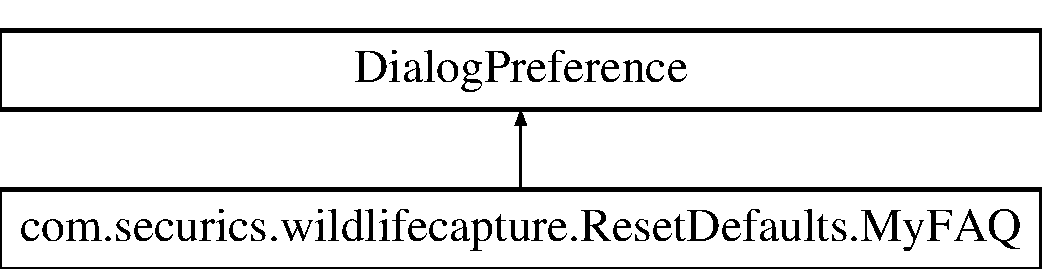
\includegraphics[height=2.000000cm]{classcom_1_1securics_1_1wildlifecapture_1_1_reset_defaults_1_1_my_f_a_q}
\end{center}
\end{figure}
\subsection*{Public Member Functions}
\begin{DoxyCompactItemize}
\item 
{\bf My\+F\+A\+Q} ()
\item 
{\bf My\+F\+A\+Q} (Context context, Attribute\+Set attrs, int def\+Style)
\item 
{\bf My\+F\+A\+Q} (Context context, Attribute\+Set attrs)
\item 
void {\bf set\+Text} (String text)
\item 
String {\bf get\+Text} ()
\item 
void {\bf on\+Click} (Dialog\+Interface dialog, int which)
\end{DoxyCompactItemize}
\subsection*{Protected Member Functions}
\begin{DoxyCompactItemize}
\item 
View {\bf on\+Create\+Dialog\+View} ()
\item 
void {\bf on\+Bind\+Dialog\+View} (View view)
\end{DoxyCompactItemize}
\subsection*{Private Member Functions}
\begin{DoxyCompactItemize}
\item 
boolean {\bf reset\+All\+Settings} ()
\end{DoxyCompactItemize}
\subsection*{Private Attributes}
\begin{DoxyCompactItemize}
\item 
Text\+View {\bf m\+Edit\+Text}
\item 
String {\bf m\+Text}
\end{DoxyCompactItemize}


\subsection{Detailed Description}


Definition at line 44 of file Reset\+Defaults.\+java.



\subsection{Constructor \& Destructor Documentation}
\index{com\+::securics\+::wildlifecapture\+::\+Reset\+Defaults\+::\+My\+F\+A\+Q@{com\+::securics\+::wildlifecapture\+::\+Reset\+Defaults\+::\+My\+F\+A\+Q}!My\+F\+A\+Q@{My\+F\+A\+Q}}
\index{My\+F\+A\+Q@{My\+F\+A\+Q}!com\+::securics\+::wildlifecapture\+::\+Reset\+Defaults\+::\+My\+F\+A\+Q@{com\+::securics\+::wildlifecapture\+::\+Reset\+Defaults\+::\+My\+F\+A\+Q}}
\subsubsection[{My\+F\+A\+Q}]{\setlength{\rightskip}{0pt plus 5cm}com.\+securics.\+wildlifecapture.\+Reset\+Defaults.\+My\+F\+A\+Q.\+My\+F\+A\+Q (
\begin{DoxyParamCaption}
{}
\end{DoxyParamCaption}
)}\label{classcom_1_1securics_1_1wildlifecapture_1_1_reset_defaults_1_1_my_f_a_q_ae9b71c18e06a728a6af50e677e3485f2}
Initialize question and answer. Set dialog title and title to variable question, set summary to Reset All Settings, and text to variable answer 

Definition at line 52 of file Reset\+Defaults.\+java.



References com.\+securics.\+wildlifecapture.\+Reset\+Defaults.\+My\+F\+A\+Q.\+set\+Text().

\index{com\+::securics\+::wildlifecapture\+::\+Reset\+Defaults\+::\+My\+F\+A\+Q@{com\+::securics\+::wildlifecapture\+::\+Reset\+Defaults\+::\+My\+F\+A\+Q}!My\+F\+A\+Q@{My\+F\+A\+Q}}
\index{My\+F\+A\+Q@{My\+F\+A\+Q}!com\+::securics\+::wildlifecapture\+::\+Reset\+Defaults\+::\+My\+F\+A\+Q@{com\+::securics\+::wildlifecapture\+::\+Reset\+Defaults\+::\+My\+F\+A\+Q}}
\subsubsection[{My\+F\+A\+Q}]{\setlength{\rightskip}{0pt plus 5cm}com.\+securics.\+wildlifecapture.\+Reset\+Defaults.\+My\+F\+A\+Q.\+My\+F\+A\+Q (
\begin{DoxyParamCaption}
\item[{Context}]{context, }
\item[{Attribute\+Set}]{attrs, }
\item[{int}]{def\+Style}
\end{DoxyParamCaption}
)}\label{classcom_1_1securics_1_1wildlifecapture_1_1_reset_defaults_1_1_my_f_a_q_a6044dd0608d13ee82ae68c8eb9534290}
Uses function super to call parent constructor with parameters context, attrs, and def\+Style 
\begin{DoxyParams}{Parameters}
{\em context} & \\
\hline
{\em attrs} & \\
\hline
{\em def\+Style} & \\
\hline
\end{DoxyParams}


Definition at line 70 of file Reset\+Defaults.\+java.

\index{com\+::securics\+::wildlifecapture\+::\+Reset\+Defaults\+::\+My\+F\+A\+Q@{com\+::securics\+::wildlifecapture\+::\+Reset\+Defaults\+::\+My\+F\+A\+Q}!My\+F\+A\+Q@{My\+F\+A\+Q}}
\index{My\+F\+A\+Q@{My\+F\+A\+Q}!com\+::securics\+::wildlifecapture\+::\+Reset\+Defaults\+::\+My\+F\+A\+Q@{com\+::securics\+::wildlifecapture\+::\+Reset\+Defaults\+::\+My\+F\+A\+Q}}
\subsubsection[{My\+F\+A\+Q}]{\setlength{\rightskip}{0pt plus 5cm}com.\+securics.\+wildlifecapture.\+Reset\+Defaults.\+My\+F\+A\+Q.\+My\+F\+A\+Q (
\begin{DoxyParamCaption}
\item[{Context}]{context, }
\item[{Attribute\+Set}]{attrs}
\end{DoxyParamCaption}
)}\label{classcom_1_1securics_1_1wildlifecapture_1_1_reset_defaults_1_1_my_f_a_q_a0ef29ced67de275507d3596c00897d85}
Uses function super to call parent constructor with parameters context and attrs 
\begin{DoxyParams}{Parameters}
{\em context} & \\
\hline
{\em attrs} & \\
\hline
\end{DoxyParams}


Definition at line 79 of file Reset\+Defaults.\+java.



\subsection{Member Function Documentation}
\index{com\+::securics\+::wildlifecapture\+::\+Reset\+Defaults\+::\+My\+F\+A\+Q@{com\+::securics\+::wildlifecapture\+::\+Reset\+Defaults\+::\+My\+F\+A\+Q}!get\+Text@{get\+Text}}
\index{get\+Text@{get\+Text}!com\+::securics\+::wildlifecapture\+::\+Reset\+Defaults\+::\+My\+F\+A\+Q@{com\+::securics\+::wildlifecapture\+::\+Reset\+Defaults\+::\+My\+F\+A\+Q}}
\subsubsection[{get\+Text}]{\setlength{\rightskip}{0pt plus 5cm}String com.\+securics.\+wildlifecapture.\+Reset\+Defaults.\+My\+F\+A\+Q.\+get\+Text (
\begin{DoxyParamCaption}
{}
\end{DoxyParamCaption}
)}\label{classcom_1_1securics_1_1wildlifecapture_1_1_reset_defaults_1_1_my_f_a_q_a74c694db55216c6311f2b465debac972}
Returns m\+Text \begin{DoxyReturn}{Returns}

\end{DoxyReturn}


Definition at line 105 of file Reset\+Defaults.\+java.



References com.\+securics.\+wildlifecapture.\+Reset\+Defaults.\+My\+F\+A\+Q.\+m\+Text.

\index{com\+::securics\+::wildlifecapture\+::\+Reset\+Defaults\+::\+My\+F\+A\+Q@{com\+::securics\+::wildlifecapture\+::\+Reset\+Defaults\+::\+My\+F\+A\+Q}!on\+Bind\+Dialog\+View@{on\+Bind\+Dialog\+View}}
\index{on\+Bind\+Dialog\+View@{on\+Bind\+Dialog\+View}!com\+::securics\+::wildlifecapture\+::\+Reset\+Defaults\+::\+My\+F\+A\+Q@{com\+::securics\+::wildlifecapture\+::\+Reset\+Defaults\+::\+My\+F\+A\+Q}}
\subsubsection[{on\+Bind\+Dialog\+View}]{\setlength{\rightskip}{0pt plus 5cm}void com.\+securics.\+wildlifecapture.\+Reset\+Defaults.\+My\+F\+A\+Q.\+on\+Bind\+Dialog\+View (
\begin{DoxyParamCaption}
\item[{View}]{view}
\end{DoxyParamCaption}
)\hspace{0.3cm}{\ttfamily [protected]}}\label{classcom_1_1securics_1_1wildlifecapture_1_1_reset_defaults_1_1_my_f_a_q_a5304c34ad96f644c099a2ad44243e084}
Set m\+Text as text for m\+Edit\+Text 

Definition at line 113 of file Reset\+Defaults.\+java.



References com.\+securics.\+wildlifecapture.\+Reset\+Defaults.\+My\+F\+A\+Q.\+m\+Text.

\index{com\+::securics\+::wildlifecapture\+::\+Reset\+Defaults\+::\+My\+F\+A\+Q@{com\+::securics\+::wildlifecapture\+::\+Reset\+Defaults\+::\+My\+F\+A\+Q}!on\+Click@{on\+Click}}
\index{on\+Click@{on\+Click}!com\+::securics\+::wildlifecapture\+::\+Reset\+Defaults\+::\+My\+F\+A\+Q@{com\+::securics\+::wildlifecapture\+::\+Reset\+Defaults\+::\+My\+F\+A\+Q}}
\subsubsection[{on\+Click}]{\setlength{\rightskip}{0pt plus 5cm}void com.\+securics.\+wildlifecapture.\+Reset\+Defaults.\+My\+F\+A\+Q.\+on\+Click (
\begin{DoxyParamCaption}
\item[{Dialog\+Interface}]{dialog, }
\item[{int}]{which}
\end{DoxyParamCaption}
)}\label{classcom_1_1securics_1_1wildlifecapture_1_1_reset_defaults_1_1_my_f_a_q_a71774d88d3d6c779fb3a58e6b090837e}
Manage feedback from buttons 

Definition at line 121 of file Reset\+Defaults.\+java.



References com.\+securics.\+wildlifecapture.\+Reset\+Defaults.\+My\+F\+A\+Q.\+m\+Text, and com.\+securics.\+wildlifecapture.\+Reset\+Defaults.\+My\+F\+A\+Q.\+reset\+All\+Settings().

\index{com\+::securics\+::wildlifecapture\+::\+Reset\+Defaults\+::\+My\+F\+A\+Q@{com\+::securics\+::wildlifecapture\+::\+Reset\+Defaults\+::\+My\+F\+A\+Q}!on\+Create\+Dialog\+View@{on\+Create\+Dialog\+View}}
\index{on\+Create\+Dialog\+View@{on\+Create\+Dialog\+View}!com\+::securics\+::wildlifecapture\+::\+Reset\+Defaults\+::\+My\+F\+A\+Q@{com\+::securics\+::wildlifecapture\+::\+Reset\+Defaults\+::\+My\+F\+A\+Q}}
\subsubsection[{on\+Create\+Dialog\+View}]{\setlength{\rightskip}{0pt plus 5cm}View com.\+securics.\+wildlifecapture.\+Reset\+Defaults.\+My\+F\+A\+Q.\+on\+Create\+Dialog\+View (
\begin{DoxyParamCaption}
{}
\end{DoxyParamCaption}
)\hspace{0.3cm}{\ttfamily [protected]}}\label{classcom_1_1securics_1_1wildlifecapture_1_1_reset_defaults_1_1_my_f_a_q_aba335777e02985182b701d13b736b089}


Definition at line 86 of file Reset\+Defaults.\+java.



References com.\+securics.\+wildlifecapture.\+Reset\+Defaults.\+My\+F\+A\+Q.\+m\+Edit\+Text.

\index{com\+::securics\+::wildlifecapture\+::\+Reset\+Defaults\+::\+My\+F\+A\+Q@{com\+::securics\+::wildlifecapture\+::\+Reset\+Defaults\+::\+My\+F\+A\+Q}!reset\+All\+Settings@{reset\+All\+Settings}}
\index{reset\+All\+Settings@{reset\+All\+Settings}!com\+::securics\+::wildlifecapture\+::\+Reset\+Defaults\+::\+My\+F\+A\+Q@{com\+::securics\+::wildlifecapture\+::\+Reset\+Defaults\+::\+My\+F\+A\+Q}}
\subsubsection[{reset\+All\+Settings}]{\setlength{\rightskip}{0pt plus 5cm}boolean com.\+securics.\+wildlifecapture.\+Reset\+Defaults.\+My\+F\+A\+Q.\+reset\+All\+Settings (
\begin{DoxyParamCaption}
{}
\end{DoxyParamCaption}
)\hspace{0.3cm}{\ttfamily [private]}}\label{classcom_1_1securics_1_1wildlifecapture_1_1_reset_defaults_1_1_my_f_a_q_ae37cb8c3c297495e71a9a6033e1ec899}
Resets squirrel and window params, camera, schedule, capture Schedule settings and file and folder locations to default. \begin{DoxyReturn}{Returns}

\end{DoxyReturn}
General Squirrel Params

Sliding Window Params

Camera Settings

Capture Schedule Settings

File and Folder locations 

Definition at line 142 of file Reset\+Defaults.\+java.



Referenced by com.\+securics.\+wildlifecapture.\+Reset\+Defaults.\+My\+F\+A\+Q.\+on\+Click().

\index{com\+::securics\+::wildlifecapture\+::\+Reset\+Defaults\+::\+My\+F\+A\+Q@{com\+::securics\+::wildlifecapture\+::\+Reset\+Defaults\+::\+My\+F\+A\+Q}!set\+Text@{set\+Text}}
\index{set\+Text@{set\+Text}!com\+::securics\+::wildlifecapture\+::\+Reset\+Defaults\+::\+My\+F\+A\+Q@{com\+::securics\+::wildlifecapture\+::\+Reset\+Defaults\+::\+My\+F\+A\+Q}}
\subsubsection[{set\+Text}]{\setlength{\rightskip}{0pt plus 5cm}void com.\+securics.\+wildlifecapture.\+Reset\+Defaults.\+My\+F\+A\+Q.\+set\+Text (
\begin{DoxyParamCaption}
\item[{String}]{text}
\end{DoxyParamCaption}
)}\label{classcom_1_1securics_1_1wildlifecapture_1_1_reset_defaults_1_1_my_f_a_q_ad906e2800fc99b1e3845fdeb1de493ca}
Set m\+Text to text 
\begin{DoxyParams}{Parameters}
{\em text} & \\
\hline
\end{DoxyParams}


Definition at line 97 of file Reset\+Defaults.\+java.



References com.\+securics.\+wildlifecapture.\+Reset\+Defaults.\+My\+F\+A\+Q.\+m\+Text.



Referenced by com.\+securics.\+wildlifecapture.\+Reset\+Defaults.\+My\+F\+A\+Q.\+My\+F\+A\+Q().



\subsection{Member Data Documentation}
\index{com\+::securics\+::wildlifecapture\+::\+Reset\+Defaults\+::\+My\+F\+A\+Q@{com\+::securics\+::wildlifecapture\+::\+Reset\+Defaults\+::\+My\+F\+A\+Q}!m\+Edit\+Text@{m\+Edit\+Text}}
\index{m\+Edit\+Text@{m\+Edit\+Text}!com\+::securics\+::wildlifecapture\+::\+Reset\+Defaults\+::\+My\+F\+A\+Q@{com\+::securics\+::wildlifecapture\+::\+Reset\+Defaults\+::\+My\+F\+A\+Q}}
\subsubsection[{m\+Edit\+Text}]{\setlength{\rightskip}{0pt plus 5cm}Text\+View com.\+securics.\+wildlifecapture.\+Reset\+Defaults.\+My\+F\+A\+Q.\+m\+Edit\+Text\hspace{0.3cm}{\ttfamily [private]}}\label{classcom_1_1securics_1_1wildlifecapture_1_1_reset_defaults_1_1_my_f_a_q_ada542bd0df087ab8195338a144c4023c}


Definition at line 83 of file Reset\+Defaults.\+java.



Referenced by com.\+securics.\+wildlifecapture.\+Reset\+Defaults.\+My\+F\+A\+Q.\+on\+Create\+Dialog\+View().

\index{com\+::securics\+::wildlifecapture\+::\+Reset\+Defaults\+::\+My\+F\+A\+Q@{com\+::securics\+::wildlifecapture\+::\+Reset\+Defaults\+::\+My\+F\+A\+Q}!m\+Text@{m\+Text}}
\index{m\+Text@{m\+Text}!com\+::securics\+::wildlifecapture\+::\+Reset\+Defaults\+::\+My\+F\+A\+Q@{com\+::securics\+::wildlifecapture\+::\+Reset\+Defaults\+::\+My\+F\+A\+Q}}
\subsubsection[{m\+Text}]{\setlength{\rightskip}{0pt plus 5cm}String com.\+securics.\+wildlifecapture.\+Reset\+Defaults.\+My\+F\+A\+Q.\+m\+Text\hspace{0.3cm}{\ttfamily [private]}}\label{classcom_1_1securics_1_1wildlifecapture_1_1_reset_defaults_1_1_my_f_a_q_a240493c3b41a7b71bbed4fdd4e25a89a}


Definition at line 92 of file Reset\+Defaults.\+java.



Referenced by com.\+securics.\+wildlifecapture.\+Reset\+Defaults.\+My\+F\+A\+Q.\+get\+Text(), com.\+securics.\+wildlifecapture.\+Reset\+Defaults.\+My\+F\+A\+Q.\+on\+Bind\+Dialog\+View(), com.\+securics.\+wildlifecapture.\+Reset\+Defaults.\+My\+F\+A\+Q.\+on\+Click(), and com.\+securics.\+wildlifecapture.\+Reset\+Defaults.\+My\+F\+A\+Q.\+set\+Text().



The documentation for this class was generated from the following file\+:\begin{DoxyCompactItemize}
\item 
src/com/securics/wildlifecapture/{\bf Reset\+Defaults.\+java}\end{DoxyCompactItemize}

\section{com.\+securics.\+wildlifecapture.\+Camera\+Preference.\+My\+List Class Reference}
\label{classcom_1_1securics_1_1wildlifecapture_1_1_camera_preference_1_1_my_list}\index{com.\+securics.\+wildlifecapture.\+Camera\+Preference.\+My\+List@{com.\+securics.\+wildlifecapture.\+Camera\+Preference.\+My\+List}}
Inheritance diagram for com.\+securics.\+wildlifecapture.\+Camera\+Preference.\+My\+List\+:\begin{figure}[H]
\begin{center}
\leavevmode
\includegraphics[height=2.000000cm]{classcom_1_1securics_1_1wildlifecapture_1_1_camera_preference_1_1_my_list}
\end{center}
\end{figure}
\subsection*{Public Member Functions}
\begin{DoxyCompactItemize}
\item 
{\bf My\+List} (int m)
\item 
{\bf My\+List} (Context context, Attribute\+Set attrs)
\end{DoxyCompactItemize}
\subsection*{Private Member Functions}
\begin{DoxyCompactItemize}
\item 
void {\bf my\+Mode} (int m)
\end{DoxyCompactItemize}


\subsection{Detailed Description}


Definition at line 65 of file Camera\+Preference.\+java.



\subsection{Constructor \& Destructor Documentation}
\index{com\+::securics\+::wildlifecapture\+::\+Camera\+Preference\+::\+My\+List@{com\+::securics\+::wildlifecapture\+::\+Camera\+Preference\+::\+My\+List}!My\+List@{My\+List}}
\index{My\+List@{My\+List}!com\+::securics\+::wildlifecapture\+::\+Camera\+Preference\+::\+My\+List@{com\+::securics\+::wildlifecapture\+::\+Camera\+Preference\+::\+My\+List}}
\subsubsection[{My\+List}]{\setlength{\rightskip}{0pt plus 5cm}com.\+securics.\+wildlifecapture.\+Camera\+Preference.\+My\+List.\+My\+List (
\begin{DoxyParamCaption}
\item[{int}]{m}
\end{DoxyParamCaption}
)}\label{classcom_1_1securics_1_1wildlifecapture_1_1_camera_preference_1_1_my_list_adeac1e58b982af057b7852f4c8352b5e}
Set entries, entry values, title to my\+Title and button text 
\begin{DoxyParams}{Parameters}
{\em m} & \\
\hline
\end{DoxyParams}


Definition at line 75 of file Camera\+Preference.\+java.



References com.\+securics.\+wildlifecapture.\+Camera\+Preference.\+My\+List.\+my\+Mode().

\index{com\+::securics\+::wildlifecapture\+::\+Camera\+Preference\+::\+My\+List@{com\+::securics\+::wildlifecapture\+::\+Camera\+Preference\+::\+My\+List}!My\+List@{My\+List}}
\index{My\+List@{My\+List}!com\+::securics\+::wildlifecapture\+::\+Camera\+Preference\+::\+My\+List@{com\+::securics\+::wildlifecapture\+::\+Camera\+Preference\+::\+My\+List}}
\subsubsection[{My\+List}]{\setlength{\rightskip}{0pt plus 5cm}com.\+securics.\+wildlifecapture.\+Camera\+Preference.\+My\+List.\+My\+List (
\begin{DoxyParamCaption}
\item[{Context}]{context, }
\item[{Attribute\+Set}]{attrs}
\end{DoxyParamCaption}
)}\label{classcom_1_1securics_1_1wildlifecapture_1_1_camera_preference_1_1_my_list_adbf5f1d85cd43202839ba780ca1baa63}
Set entries, entry values, title to my\+Title and button text 
\begin{DoxyParams}{Parameters}
{\em context} & \\
\hline
{\em attrs} & \\
\hline
\end{DoxyParams}


Definition at line 91 of file Camera\+Preference.\+java.



\subsection{Member Function Documentation}
\index{com\+::securics\+::wildlifecapture\+::\+Camera\+Preference\+::\+My\+List@{com\+::securics\+::wildlifecapture\+::\+Camera\+Preference\+::\+My\+List}!my\+Mode@{my\+Mode}}
\index{my\+Mode@{my\+Mode}!com\+::securics\+::wildlifecapture\+::\+Camera\+Preference\+::\+My\+List@{com\+::securics\+::wildlifecapture\+::\+Camera\+Preference\+::\+My\+List}}
\subsubsection[{my\+Mode}]{\setlength{\rightskip}{0pt plus 5cm}void com.\+securics.\+wildlifecapture.\+Camera\+Preference.\+My\+List.\+my\+Mode (
\begin{DoxyParamCaption}
\item[{int}]{m}
\end{DoxyParamCaption}
)\hspace{0.3cm}{\ttfamily [private]}}\label{classcom_1_1securics_1_1wildlifecapture_1_1_camera_preference_1_1_my_list_abdd8a7dff5f858e544efbc777f79f977}
Uses a switch to set variables accordingly 
\begin{DoxyParams}{Parameters}
{\em m} & \\
\hline
\end{DoxyParams}


Definition at line 101 of file Camera\+Preference.\+java.



Referenced by com.\+securics.\+wildlifecapture.\+Camera\+Preference.\+My\+List.\+My\+List().



The documentation for this class was generated from the following file\+:\begin{DoxyCompactItemize}
\item 
src/com/securics/wildlifecapture/{\bf Camera\+Preference.\+java}\end{DoxyCompactItemize}

\section{com.\+securics.\+wildlifecapture.\+My\+Number\+Preference Class Reference}
\label{classcom_1_1securics_1_1wildlifecapture_1_1_my_number_preference}\index{com.\+securics.\+wildlifecapture.\+My\+Number\+Preference@{com.\+securics.\+wildlifecapture.\+My\+Number\+Preference}}
Inheritance diagram for com.\+securics.\+wildlifecapture.\+My\+Number\+Preference\+:\begin{figure}[H]
\begin{center}
\leavevmode
\includegraphics[height=2.000000cm]{classcom_1_1securics_1_1wildlifecapture_1_1_my_number_preference}
\end{center}
\end{figure}
\subsection*{Public Member Functions}
\begin{DoxyCompactItemize}
\item 
{\bf My\+Number\+Preference} (Context context, Attribute\+Set attrs)
\item 
void {\bf set\+Type} (String type)
\item 
void {\bf default\+Value} (String value)
\end{DoxyCompactItemize}
\subsection*{Protected Member Functions}
\begin{DoxyCompactItemize}
\item 
void {\bf on\+Bind\+View} (View view)
\item 
void {\bf on\+Dialog\+Closed} (boolean positive\+Result)
\item 
Object {\bf on\+Get\+Default\+Value} (Typed\+Array a, int index)
\item 
void {\bf on\+Set\+Initial\+Value} (boolean restore\+Value, Object {\bf default\+Value})
\item 
Parcelable {\bf on\+Save\+Instance\+State} ()
\end{DoxyCompactItemize}
\subsection*{Private Attributes}
\begin{DoxyCompactItemize}
\item 
int {\bf saved\+Int}
\item 
float {\bf saved\+Float}
\item 
String {\bf preference\+\_\+string}
\item 
String {\bf my\+Type}
\item 
String {\bf my\+Default\+Value}
\end{DoxyCompactItemize}


\subsection{Detailed Description}


Definition at line 14 of file My\+Number\+Preference.\+java.



\subsection{Constructor \& Destructor Documentation}
\index{com\+::securics\+::wildlifecapture\+::\+My\+Number\+Preference@{com\+::securics\+::wildlifecapture\+::\+My\+Number\+Preference}!My\+Number\+Preference@{My\+Number\+Preference}}
\index{My\+Number\+Preference@{My\+Number\+Preference}!com\+::securics\+::wildlifecapture\+::\+My\+Number\+Preference@{com\+::securics\+::wildlifecapture\+::\+My\+Number\+Preference}}
\subsubsection[{My\+Number\+Preference}]{\setlength{\rightskip}{0pt plus 5cm}com.\+securics.\+wildlifecapture.\+My\+Number\+Preference.\+My\+Number\+Preference (
\begin{DoxyParamCaption}
\item[{Context}]{context, }
\item[{Attribute\+Set}]{attrs}
\end{DoxyParamCaption}
)}\label{classcom_1_1securics_1_1wildlifecapture_1_1_my_number_preference_afa839bea657f32fd9af20324477d5e62}
This is the constructor called by the inflater 
\begin{DoxyParams}{Parameters}
{\em context} & \\
\hline
{\em attrs} & \\
\hline
\end{DoxyParams}


Definition at line 26 of file My\+Number\+Preference.\+java.



References com.\+securics.\+wildlifecapture.\+My\+Number\+Preference.\+my\+Default\+Value, and com.\+securics.\+wildlifecapture.\+My\+Number\+Preference.\+my\+Type.



\subsection{Member Function Documentation}
\index{com\+::securics\+::wildlifecapture\+::\+My\+Number\+Preference@{com\+::securics\+::wildlifecapture\+::\+My\+Number\+Preference}!default\+Value@{default\+Value}}
\index{default\+Value@{default\+Value}!com\+::securics\+::wildlifecapture\+::\+My\+Number\+Preference@{com\+::securics\+::wildlifecapture\+::\+My\+Number\+Preference}}
\subsubsection[{default\+Value}]{\setlength{\rightskip}{0pt plus 5cm}void com.\+securics.\+wildlifecapture.\+My\+Number\+Preference.\+default\+Value (
\begin{DoxyParamCaption}
\item[{String}]{value}
\end{DoxyParamCaption}
)}\label{classcom_1_1securics_1_1wildlifecapture_1_1_my_number_preference_a0ee2706a6fa597368b00ed4859f61665}
Sets value of my\+Default\+Value 
\begin{DoxyParams}{Parameters}
{\em value} & \\
\hline
\end{DoxyParams}


Definition at line 45 of file My\+Number\+Preference.\+java.



References com.\+securics.\+wildlifecapture.\+My\+Number\+Preference.\+my\+Default\+Value.

\index{com\+::securics\+::wildlifecapture\+::\+My\+Number\+Preference@{com\+::securics\+::wildlifecapture\+::\+My\+Number\+Preference}!on\+Bind\+View@{on\+Bind\+View}}
\index{on\+Bind\+View@{on\+Bind\+View}!com\+::securics\+::wildlifecapture\+::\+My\+Number\+Preference@{com\+::securics\+::wildlifecapture\+::\+My\+Number\+Preference}}
\subsubsection[{on\+Bind\+View}]{\setlength{\rightskip}{0pt plus 5cm}void com.\+securics.\+wildlifecapture.\+My\+Number\+Preference.\+on\+Bind\+View (
\begin{DoxyParamCaption}
\item[{View}]{view}
\end{DoxyParamCaption}
)\hspace{0.3cm}{\ttfamily [protected]}}\label{classcom_1_1securics_1_1wildlifecapture_1_1_my_number_preference_a54081752a0f42804989cb480fc136af5}
Sets value of saved\+Int, saved\+Float, and preference\+\_\+string Set our custom views inside the layout 

Definition at line 54 of file My\+Number\+Preference.\+java.



References com.\+securics.\+wildlifecapture.\+Main\+Activity.\+debug\+Mode, com.\+securics.\+wildlifecapture.\+My\+Number\+Preference.\+my\+Default\+Value, com.\+securics.\+wildlifecapture.\+My\+Number\+Preference.\+my\+Type, com.\+securics.\+wildlifecapture.\+My\+Number\+Preference.\+preference\+\_\+string, com.\+securics.\+wildlifecapture.\+My\+Number\+Preference.\+saved\+Float, and com.\+securics.\+wildlifecapture.\+My\+Number\+Preference.\+saved\+Int.

\index{com\+::securics\+::wildlifecapture\+::\+My\+Number\+Preference@{com\+::securics\+::wildlifecapture\+::\+My\+Number\+Preference}!on\+Dialog\+Closed@{on\+Dialog\+Closed}}
\index{on\+Dialog\+Closed@{on\+Dialog\+Closed}!com\+::securics\+::wildlifecapture\+::\+My\+Number\+Preference@{com\+::securics\+::wildlifecapture\+::\+My\+Number\+Preference}}
\subsubsection[{on\+Dialog\+Closed}]{\setlength{\rightskip}{0pt plus 5cm}void com.\+securics.\+wildlifecapture.\+My\+Number\+Preference.\+on\+Dialog\+Closed (
\begin{DoxyParamCaption}
\item[{boolean}]{positive\+Result}
\end{DoxyParamCaption}
)\hspace{0.3cm}{\ttfamily [protected]}}\label{classcom_1_1securics_1_1wildlifecapture_1_1_my_number_preference_acb9441e2afd78c1f7b683fac2567ec25}
Saved value of saved\+Float, saved\+Int 

Definition at line 97 of file My\+Number\+Preference.\+java.



References com.\+securics.\+wildlifecapture.\+Main\+Activity.\+debug\+Mode, com.\+securics.\+wildlifecapture.\+My\+Number\+Preference.\+my\+Type, com.\+securics.\+wildlifecapture.\+My\+Number\+Preference.\+preference\+\_\+string, com.\+securics.\+wildlifecapture.\+My\+Number\+Preference.\+saved\+Float, and com.\+securics.\+wildlifecapture.\+My\+Number\+Preference.\+saved\+Int.

\index{com\+::securics\+::wildlifecapture\+::\+My\+Number\+Preference@{com\+::securics\+::wildlifecapture\+::\+My\+Number\+Preference}!on\+Get\+Default\+Value@{on\+Get\+Default\+Value}}
\index{on\+Get\+Default\+Value@{on\+Get\+Default\+Value}!com\+::securics\+::wildlifecapture\+::\+My\+Number\+Preference@{com\+::securics\+::wildlifecapture\+::\+My\+Number\+Preference}}
\subsubsection[{on\+Get\+Default\+Value}]{\setlength{\rightskip}{0pt plus 5cm}Object com.\+securics.\+wildlifecapture.\+My\+Number\+Preference.\+on\+Get\+Default\+Value (
\begin{DoxyParamCaption}
\item[{Typed\+Array}]{a, }
\item[{int}]{index}
\end{DoxyParamCaption}
)\hspace{0.3cm}{\ttfamily [protected]}}\label{classcom_1_1securics_1_1wildlifecapture_1_1_my_number_preference_af144dd1622ac21ec4af131194876548a}
This preference type's value type is Integer, so we read the default value from the attributes as an Integer.

Definition at line 134 of file My\+Number\+Preference.\+java.

\index{com\+::securics\+::wildlifecapture\+::\+My\+Number\+Preference@{com\+::securics\+::wildlifecapture\+::\+My\+Number\+Preference}!on\+Save\+Instance\+State@{on\+Save\+Instance\+State}}
\index{on\+Save\+Instance\+State@{on\+Save\+Instance\+State}!com\+::securics\+::wildlifecapture\+::\+My\+Number\+Preference@{com\+::securics\+::wildlifecapture\+::\+My\+Number\+Preference}}
\subsubsection[{on\+Save\+Instance\+State}]{\setlength{\rightskip}{0pt plus 5cm}Parcelable com.\+securics.\+wildlifecapture.\+My\+Number\+Preference.\+on\+Save\+Instance\+State (
\begin{DoxyParamCaption}
{}
\end{DoxyParamCaption}
)\hspace{0.3cm}{\ttfamily [protected]}}\label{classcom_1_1securics_1_1wildlifecapture_1_1_my_number_preference_ac6ada6f2bc105508e4324367c488f636}
Suppose a client uses this preference type without persisting. We must save the instance state so it is able to, for example, survive orientation changes.

Definition at line 161 of file My\+Number\+Preference.\+java.

\index{com\+::securics\+::wildlifecapture\+::\+My\+Number\+Preference@{com\+::securics\+::wildlifecapture\+::\+My\+Number\+Preference}!on\+Set\+Initial\+Value@{on\+Set\+Initial\+Value}}
\index{on\+Set\+Initial\+Value@{on\+Set\+Initial\+Value}!com\+::securics\+::wildlifecapture\+::\+My\+Number\+Preference@{com\+::securics\+::wildlifecapture\+::\+My\+Number\+Preference}}
\subsubsection[{on\+Set\+Initial\+Value}]{\setlength{\rightskip}{0pt plus 5cm}void com.\+securics.\+wildlifecapture.\+My\+Number\+Preference.\+on\+Set\+Initial\+Value (
\begin{DoxyParamCaption}
\item[{boolean}]{restore\+Value, }
\item[{Object}]{default\+Value}
\end{DoxyParamCaption}
)\hspace{0.3cm}{\ttfamily [protected]}}\label{classcom_1_1securics_1_1wildlifecapture_1_1_my_number_preference_a836d3fc75d81dd67b9184b9d5beb0c16}
Set value to prefrence\+\_\+string 

Definition at line 147 of file My\+Number\+Preference.\+java.



References com.\+securics.\+wildlifecapture.\+My\+Number\+Preference.\+preference\+\_\+string.

\index{com\+::securics\+::wildlifecapture\+::\+My\+Number\+Preference@{com\+::securics\+::wildlifecapture\+::\+My\+Number\+Preference}!set\+Type@{set\+Type}}
\index{set\+Type@{set\+Type}!com\+::securics\+::wildlifecapture\+::\+My\+Number\+Preference@{com\+::securics\+::wildlifecapture\+::\+My\+Number\+Preference}}
\subsubsection[{set\+Type}]{\setlength{\rightskip}{0pt plus 5cm}void com.\+securics.\+wildlifecapture.\+My\+Number\+Preference.\+set\+Type (
\begin{DoxyParamCaption}
\item[{String}]{type}
\end{DoxyParamCaption}
)}\label{classcom_1_1securics_1_1wildlifecapture_1_1_my_number_preference_aafde84d2df6b4b28590b36a5a012db53}
Sets value of my\+Type 
\begin{DoxyParams}{Parameters}
{\em type} & \\
\hline
\end{DoxyParams}


Definition at line 37 of file My\+Number\+Preference.\+java.



References com.\+securics.\+wildlifecapture.\+My\+Number\+Preference.\+my\+Type.



Referenced by com.\+securics.\+wildlifecapture.\+General\+Settings.\+load\+Params().



\subsection{Member Data Documentation}
\index{com\+::securics\+::wildlifecapture\+::\+My\+Number\+Preference@{com\+::securics\+::wildlifecapture\+::\+My\+Number\+Preference}!my\+Default\+Value@{my\+Default\+Value}}
\index{my\+Default\+Value@{my\+Default\+Value}!com\+::securics\+::wildlifecapture\+::\+My\+Number\+Preference@{com\+::securics\+::wildlifecapture\+::\+My\+Number\+Preference}}
\subsubsection[{my\+Default\+Value}]{\setlength{\rightskip}{0pt plus 5cm}String com.\+securics.\+wildlifecapture.\+My\+Number\+Preference.\+my\+Default\+Value\hspace{0.3cm}{\ttfamily [private]}}\label{classcom_1_1securics_1_1wildlifecapture_1_1_my_number_preference_a652eb24d0d2caa9835b81ebb6bd468cc}


Definition at line 19 of file My\+Number\+Preference.\+java.



Referenced by com.\+securics.\+wildlifecapture.\+My\+Number\+Preference.\+default\+Value(), com.\+securics.\+wildlifecapture.\+My\+Number\+Preference.\+My\+Number\+Preference(), and com.\+securics.\+wildlifecapture.\+My\+Number\+Preference.\+on\+Bind\+View().

\index{com\+::securics\+::wildlifecapture\+::\+My\+Number\+Preference@{com\+::securics\+::wildlifecapture\+::\+My\+Number\+Preference}!my\+Type@{my\+Type}}
\index{my\+Type@{my\+Type}!com\+::securics\+::wildlifecapture\+::\+My\+Number\+Preference@{com\+::securics\+::wildlifecapture\+::\+My\+Number\+Preference}}
\subsubsection[{my\+Type}]{\setlength{\rightskip}{0pt plus 5cm}String com.\+securics.\+wildlifecapture.\+My\+Number\+Preference.\+my\+Type\hspace{0.3cm}{\ttfamily [private]}}\label{classcom_1_1securics_1_1wildlifecapture_1_1_my_number_preference_aae6a127ad2be3196f1c4bf0b3590b6d5}


Definition at line 18 of file My\+Number\+Preference.\+java.



Referenced by com.\+securics.\+wildlifecapture.\+My\+Number\+Preference.\+My\+Number\+Preference(), com.\+securics.\+wildlifecapture.\+My\+Number\+Preference.\+on\+Bind\+View(), com.\+securics.\+wildlifecapture.\+My\+Number\+Preference.\+on\+Dialog\+Closed(), and com.\+securics.\+wildlifecapture.\+My\+Number\+Preference.\+set\+Type().

\index{com\+::securics\+::wildlifecapture\+::\+My\+Number\+Preference@{com\+::securics\+::wildlifecapture\+::\+My\+Number\+Preference}!preference\+\_\+string@{preference\+\_\+string}}
\index{preference\+\_\+string@{preference\+\_\+string}!com\+::securics\+::wildlifecapture\+::\+My\+Number\+Preference@{com\+::securics\+::wildlifecapture\+::\+My\+Number\+Preference}}
\subsubsection[{preference\+\_\+string}]{\setlength{\rightskip}{0pt plus 5cm}String com.\+securics.\+wildlifecapture.\+My\+Number\+Preference.\+preference\+\_\+string\hspace{0.3cm}{\ttfamily [private]}}\label{classcom_1_1securics_1_1wildlifecapture_1_1_my_number_preference_a203d22dff492d3707c55f9c9b66a683a}


Definition at line 17 of file My\+Number\+Preference.\+java.



Referenced by com.\+securics.\+wildlifecapture.\+My\+Number\+Preference.\+on\+Bind\+View(), com.\+securics.\+wildlifecapture.\+My\+Number\+Preference.\+on\+Dialog\+Closed(), and com.\+securics.\+wildlifecapture.\+My\+Number\+Preference.\+on\+Set\+Initial\+Value().

\index{com\+::securics\+::wildlifecapture\+::\+My\+Number\+Preference@{com\+::securics\+::wildlifecapture\+::\+My\+Number\+Preference}!saved\+Float@{saved\+Float}}
\index{saved\+Float@{saved\+Float}!com\+::securics\+::wildlifecapture\+::\+My\+Number\+Preference@{com\+::securics\+::wildlifecapture\+::\+My\+Number\+Preference}}
\subsubsection[{saved\+Float}]{\setlength{\rightskip}{0pt plus 5cm}float com.\+securics.\+wildlifecapture.\+My\+Number\+Preference.\+saved\+Float\hspace{0.3cm}{\ttfamily [private]}}\label{classcom_1_1securics_1_1wildlifecapture_1_1_my_number_preference_a10e883f833b5c6e16af1df7d7eef3660}


Definition at line 16 of file My\+Number\+Preference.\+java.



Referenced by com.\+securics.\+wildlifecapture.\+My\+Number\+Preference.\+on\+Bind\+View(), and com.\+securics.\+wildlifecapture.\+My\+Number\+Preference.\+on\+Dialog\+Closed().

\index{com\+::securics\+::wildlifecapture\+::\+My\+Number\+Preference@{com\+::securics\+::wildlifecapture\+::\+My\+Number\+Preference}!saved\+Int@{saved\+Int}}
\index{saved\+Int@{saved\+Int}!com\+::securics\+::wildlifecapture\+::\+My\+Number\+Preference@{com\+::securics\+::wildlifecapture\+::\+My\+Number\+Preference}}
\subsubsection[{saved\+Int}]{\setlength{\rightskip}{0pt plus 5cm}int com.\+securics.\+wildlifecapture.\+My\+Number\+Preference.\+saved\+Int\hspace{0.3cm}{\ttfamily [private]}}\label{classcom_1_1securics_1_1wildlifecapture_1_1_my_number_preference_a2dccaafe974075a0be7670dd48d73d95}


Definition at line 15 of file My\+Number\+Preference.\+java.



Referenced by com.\+securics.\+wildlifecapture.\+My\+Number\+Preference.\+on\+Bind\+View(), and com.\+securics.\+wildlifecapture.\+My\+Number\+Preference.\+on\+Dialog\+Closed().



The documentation for this class was generated from the following file\+:\begin{DoxyCompactItemize}
\item 
src/com/securics/wildlifecapture/{\bf My\+Number\+Preference.\+java}\end{DoxyCompactItemize}

\section{com.\+securics.\+wildlifecapture.\+My\+String\+Preference Class Reference}
\label{classcom_1_1securics_1_1wildlifecapture_1_1_my_string_preference}\index{com.\+securics.\+wildlifecapture.\+My\+String\+Preference@{com.\+securics.\+wildlifecapture.\+My\+String\+Preference}}
Inheritance diagram for com.\+securics.\+wildlifecapture.\+My\+String\+Preference\+:\begin{figure}[H]
\begin{center}
\leavevmode
\includegraphics[height=2.000000cm]{classcom_1_1securics_1_1wildlifecapture_1_1_my_string_preference}
\end{center}
\end{figure}
\subsection*{Classes}
\begin{DoxyCompactItemize}
\item 
class {\bfseries Saved\+State}
\end{DoxyCompactItemize}
\subsection*{Public Member Functions}
\begin{DoxyCompactItemize}
\item 
{\bf My\+String\+Preference} (Context context, Attribute\+Set attrs)
\end{DoxyCompactItemize}
\subsection*{Protected Member Functions}
\begin{DoxyCompactItemize}
\item 
void {\bf on\+Bind\+View} (View view)
\item 
void {\bf on\+Dialog\+Closed} (boolean positive\+Result)
\item 
Object {\bf on\+Get\+Default\+Value} (Typed\+Array a, int index)
\item 
void {\bf on\+Set\+Initial\+Value} (boolean restore\+Value, Object default\+Value)
\item 
Parcelable {\bf on\+Save\+Instance\+State} ()
\item 
void {\bf on\+Restore\+Instance\+State} (Parcelable state)
\end{DoxyCompactItemize}
\subsection*{Private Attributes}
\begin{DoxyCompactItemize}
\item 
String {\bf preference\+\_\+string}
\end{DoxyCompactItemize}


\subsection{Detailed Description}


Definition at line 12 of file My\+String\+Preference.\+java.



\subsection{Constructor \& Destructor Documentation}
\index{com\+::securics\+::wildlifecapture\+::\+My\+String\+Preference@{com\+::securics\+::wildlifecapture\+::\+My\+String\+Preference}!My\+String\+Preference@{My\+String\+Preference}}
\index{My\+String\+Preference@{My\+String\+Preference}!com\+::securics\+::wildlifecapture\+::\+My\+String\+Preference@{com\+::securics\+::wildlifecapture\+::\+My\+String\+Preference}}
\subsubsection[{My\+String\+Preference}]{\setlength{\rightskip}{0pt plus 5cm}com.\+securics.\+wildlifecapture.\+My\+String\+Preference.\+My\+String\+Preference (
\begin{DoxyParamCaption}
\item[{Context}]{context, }
\item[{Attribute\+Set}]{attrs}
\end{DoxyParamCaption}
)}\label{classcom_1_1securics_1_1wildlifecapture_1_1_my_string_preference_ae31af000f466a9ca8489d0c93aa7c3ac}
This is the constructor called by the inflater 
\begin{DoxyParams}{Parameters}
{\em context} & \\
\hline
{\em attrs} & \\
\hline
\end{DoxyParams}


Definition at line 20 of file My\+String\+Preference.\+java.



\subsection{Member Function Documentation}
\index{com\+::securics\+::wildlifecapture\+::\+My\+String\+Preference@{com\+::securics\+::wildlifecapture\+::\+My\+String\+Preference}!on\+Bind\+View@{on\+Bind\+View}}
\index{on\+Bind\+View@{on\+Bind\+View}!com\+::securics\+::wildlifecapture\+::\+My\+String\+Preference@{com\+::securics\+::wildlifecapture\+::\+My\+String\+Preference}}
\subsubsection[{on\+Bind\+View}]{\setlength{\rightskip}{0pt plus 5cm}void com.\+securics.\+wildlifecapture.\+My\+String\+Preference.\+on\+Bind\+View (
\begin{DoxyParamCaption}
\item[{View}]{view}
\end{DoxyParamCaption}
)\hspace{0.3cm}{\ttfamily [protected]}}\label{classcom_1_1securics_1_1wildlifecapture_1_1_my_string_preference_a7dc194fb959c65ae2a909741ac7e0d90}
Sets test to preference\+\_\+string if my\+Text\+View is null. If not, declare Edit\+Text\+Preference p as an extension of shared preference and let p save the value of preference\+\_\+string to it Set our custom views inside the layout 

Definition at line 32 of file My\+String\+Preference.\+java.



References com.\+securics.\+wildlifecapture.\+My\+String\+Preference.\+preference\+\_\+string.

\index{com\+::securics\+::wildlifecapture\+::\+My\+String\+Preference@{com\+::securics\+::wildlifecapture\+::\+My\+String\+Preference}!on\+Dialog\+Closed@{on\+Dialog\+Closed}}
\index{on\+Dialog\+Closed@{on\+Dialog\+Closed}!com\+::securics\+::wildlifecapture\+::\+My\+String\+Preference@{com\+::securics\+::wildlifecapture\+::\+My\+String\+Preference}}
\subsubsection[{on\+Dialog\+Closed}]{\setlength{\rightskip}{0pt plus 5cm}void com.\+securics.\+wildlifecapture.\+My\+String\+Preference.\+on\+Dialog\+Closed (
\begin{DoxyParamCaption}
\item[{boolean}]{positive\+Result}
\end{DoxyParamCaption}
)\hspace{0.3cm}{\ttfamily [protected]}}\label{classcom_1_1securics_1_1wildlifecapture_1_1_my_string_preference_a2ed32e78661c200e1686be863df572fe}
If positive\+Result is true, and preference\+\_\+string has changed, save preference\+\_\+string to Shared\+Preference 

Definition at line 49 of file My\+String\+Preference.\+java.



References com.\+securics.\+wildlifecapture.\+My\+String\+Preference.\+preference\+\_\+string.

\index{com\+::securics\+::wildlifecapture\+::\+My\+String\+Preference@{com\+::securics\+::wildlifecapture\+::\+My\+String\+Preference}!on\+Get\+Default\+Value@{on\+Get\+Default\+Value}}
\index{on\+Get\+Default\+Value@{on\+Get\+Default\+Value}!com\+::securics\+::wildlifecapture\+::\+My\+String\+Preference@{com\+::securics\+::wildlifecapture\+::\+My\+String\+Preference}}
\subsubsection[{on\+Get\+Default\+Value}]{\setlength{\rightskip}{0pt plus 5cm}Object com.\+securics.\+wildlifecapture.\+My\+String\+Preference.\+on\+Get\+Default\+Value (
\begin{DoxyParamCaption}
\item[{Typed\+Array}]{a, }
\item[{int}]{index}
\end{DoxyParamCaption}
)\hspace{0.3cm}{\ttfamily [protected]}}\label{classcom_1_1securics_1_1wildlifecapture_1_1_my_string_preference_a614d4c50889d172d4e60480042d1a05d}
This preference type's value type is Integer, so we read the default value from the attributes as an Integer.

Definition at line 63 of file My\+String\+Preference.\+java.

\index{com\+::securics\+::wildlifecapture\+::\+My\+String\+Preference@{com\+::securics\+::wildlifecapture\+::\+My\+String\+Preference}!on\+Restore\+Instance\+State@{on\+Restore\+Instance\+State}}
\index{on\+Restore\+Instance\+State@{on\+Restore\+Instance\+State}!com\+::securics\+::wildlifecapture\+::\+My\+String\+Preference@{com\+::securics\+::wildlifecapture\+::\+My\+String\+Preference}}
\subsubsection[{on\+Restore\+Instance\+State}]{\setlength{\rightskip}{0pt plus 5cm}void com.\+securics.\+wildlifecapture.\+My\+String\+Preference.\+on\+Restore\+Instance\+State (
\begin{DoxyParamCaption}
\item[{Parcelable}]{state}
\end{DoxyParamCaption}
)\hspace{0.3cm}{\ttfamily [protected]}}\label{classcom_1_1securics_1_1wildlifecapture_1_1_my_string_preference_a51af4891f592eabe3e5f4a3f0d6a6ea5}
Restores the instance state if it is not already 

Definition at line 113 of file My\+String\+Preference.\+java.



References com.\+securics.\+wildlifecapture.\+My\+String\+Preference.\+preference\+\_\+string.

\index{com\+::securics\+::wildlifecapture\+::\+My\+String\+Preference@{com\+::securics\+::wildlifecapture\+::\+My\+String\+Preference}!on\+Save\+Instance\+State@{on\+Save\+Instance\+State}}
\index{on\+Save\+Instance\+State@{on\+Save\+Instance\+State}!com\+::securics\+::wildlifecapture\+::\+My\+String\+Preference@{com\+::securics\+::wildlifecapture\+::\+My\+String\+Preference}}
\subsubsection[{on\+Save\+Instance\+State}]{\setlength{\rightskip}{0pt plus 5cm}Parcelable com.\+securics.\+wildlifecapture.\+My\+String\+Preference.\+on\+Save\+Instance\+State (
\begin{DoxyParamCaption}
{}
\end{DoxyParamCaption}
)\hspace{0.3cm}{\ttfamily [protected]}}\label{classcom_1_1securics_1_1wildlifecapture_1_1_my_string_preference_a58bdbdf1330118d01f405572631a8717}
Suppose a client uses this preference type without persisting. We must save the instance state so it is able to, for example, survive orientation changes.

Definition at line 90 of file My\+String\+Preference.\+java.



References com.\+securics.\+wildlifecapture.\+My\+String\+Preference.\+preference\+\_\+string.

\index{com\+::securics\+::wildlifecapture\+::\+My\+String\+Preference@{com\+::securics\+::wildlifecapture\+::\+My\+String\+Preference}!on\+Set\+Initial\+Value@{on\+Set\+Initial\+Value}}
\index{on\+Set\+Initial\+Value@{on\+Set\+Initial\+Value}!com\+::securics\+::wildlifecapture\+::\+My\+String\+Preference@{com\+::securics\+::wildlifecapture\+::\+My\+String\+Preference}}
\subsubsection[{on\+Set\+Initial\+Value}]{\setlength{\rightskip}{0pt plus 5cm}void com.\+securics.\+wildlifecapture.\+My\+String\+Preference.\+on\+Set\+Initial\+Value (
\begin{DoxyParamCaption}
\item[{boolean}]{restore\+Value, }
\item[{Object}]{default\+Value}
\end{DoxyParamCaption}
)\hspace{0.3cm}{\ttfamily [protected]}}\label{classcom_1_1securics_1_1wildlifecapture_1_1_my_string_preference_a142288d6b4f3df72bf6b48e94a1ad63b}
Intializes preference\+\_\+string 

Definition at line 76 of file My\+String\+Preference.\+java.



References com.\+securics.\+wildlifecapture.\+My\+String\+Preference.\+preference\+\_\+string.



\subsection{Member Data Documentation}
\index{com\+::securics\+::wildlifecapture\+::\+My\+String\+Preference@{com\+::securics\+::wildlifecapture\+::\+My\+String\+Preference}!preference\+\_\+string@{preference\+\_\+string}}
\index{preference\+\_\+string@{preference\+\_\+string}!com\+::securics\+::wildlifecapture\+::\+My\+String\+Preference@{com\+::securics\+::wildlifecapture\+::\+My\+String\+Preference}}
\subsubsection[{preference\+\_\+string}]{\setlength{\rightskip}{0pt plus 5cm}String com.\+securics.\+wildlifecapture.\+My\+String\+Preference.\+preference\+\_\+string\hspace{0.3cm}{\ttfamily [private]}}\label{classcom_1_1securics_1_1wildlifecapture_1_1_my_string_preference_ae18f2dfcbea2946ec13ba306e73077e3}


Definition at line 13 of file My\+String\+Preference.\+java.



Referenced by com.\+securics.\+wildlifecapture.\+My\+String\+Preference.\+on\+Bind\+View(), com.\+securics.\+wildlifecapture.\+My\+String\+Preference.\+on\+Dialog\+Closed(), com.\+securics.\+wildlifecapture.\+My\+String\+Preference.\+on\+Restore\+Instance\+State(), com.\+securics.\+wildlifecapture.\+My\+String\+Preference.\+on\+Save\+Instance\+State(), and com.\+securics.\+wildlifecapture.\+My\+String\+Preference.\+on\+Set\+Initial\+Value().



The documentation for this class was generated from the following file\+:\begin{DoxyCompactItemize}
\item 
src/com/securics/wildlifecapture/{\bf My\+String\+Preference.\+java}\end{DoxyCompactItemize}

\section{com.\+securics.\+wildlifecapture.\+Perspective\+Transformation\+Engine Class Reference}
\label{classcom_1_1securics_1_1wildlifecapture_1_1_perspective_transformation_engine}\index{com.\+securics.\+wildlifecapture.\+Perspective\+Transformation\+Engine@{com.\+securics.\+wildlifecapture.\+Perspective\+Transformation\+Engine}}


\subsection{Detailed Description}


Definition at line 3 of file Perspective\+Transformation\+Engine.\+java.



The documentation for this class was generated from the following file\+:\begin{DoxyCompactItemize}
\item 
src/com/securics/wildlifecapture/{\bf Perspective\+Transformation\+Engine.\+java}\end{DoxyCompactItemize}

\section{com.\+securics.\+wildlifecapture.\+Main\+Activity.\+Push\+To\+J\+N\+I\+Runnable Class Reference}
\label{classcom_1_1securics_1_1wildlifecapture_1_1_main_activity_1_1_push_to_j_n_i_runnable}\index{com.\+securics.\+wildlifecapture.\+Main\+Activity.\+Push\+To\+J\+N\+I\+Runnable@{com.\+securics.\+wildlifecapture.\+Main\+Activity.\+Push\+To\+J\+N\+I\+Runnable}}
Inheritance diagram for com.\+securics.\+wildlifecapture.\+Main\+Activity.\+Push\+To\+J\+N\+I\+Runnable\+:\begin{figure}[H]
\begin{center}
\leavevmode
\includegraphics[height=2.000000cm]{classcom_1_1securics_1_1wildlifecapture_1_1_main_activity_1_1_push_to_j_n_i_runnable}
\end{center}
\end{figure}
\subsection*{Public Member Functions}
\begin{DoxyCompactItemize}
\item 
void {\bf run} ()
\item 
void {\bf do\+Pushing} ()
\end{DoxyCompactItemize}


\subsection{Detailed Description}
Thread runnable to push data to J\+N\+I. 

Definition at line 1254 of file Main\+Activity.\+java.



\subsection{Member Function Documentation}
\index{com\+::securics\+::wildlifecapture\+::\+Main\+Activity\+::\+Push\+To\+J\+N\+I\+Runnable@{com\+::securics\+::wildlifecapture\+::\+Main\+Activity\+::\+Push\+To\+J\+N\+I\+Runnable}!do\+Pushing@{do\+Pushing}}
\index{do\+Pushing@{do\+Pushing}!com\+::securics\+::wildlifecapture\+::\+Main\+Activity\+::\+Push\+To\+J\+N\+I\+Runnable@{com\+::securics\+::wildlifecapture\+::\+Main\+Activity\+::\+Push\+To\+J\+N\+I\+Runnable}}
\subsubsection[{do\+Pushing}]{\setlength{\rightskip}{0pt plus 5cm}void com.\+securics.\+wildlifecapture.\+Main\+Activity.\+Push\+To\+J\+N\+I\+Runnable.\+do\+Pushing (
\begin{DoxyParamCaption}
{}
\end{DoxyParamCaption}
)}\label{classcom_1_1securics_1_1wildlifecapture_1_1_main_activity_1_1_push_to_j_n_i_runnable_aa0e4f21857ea4f3d0409fd4ecdcd9a5a}


Definition at line 1259 of file Main\+Activity.\+java.



References com.\+securics.\+wildlifecapture.\+Main\+Activity.\+cam, com.\+securics.\+wildlifecapture.\+Main\+Activity.\+D\+E\+A\+T\+H, com.\+securics.\+wildlifecapture.\+Main\+Activity.\+debug\+Mode, com.\+securics.\+wildlifecapture.\+Main\+Activity.\+directory, com.\+securics.\+wildlifecapture.\+Main\+Activity.\+do\+Revised\+J\+N\+I(), com.\+securics.\+wildlifecapture.\+Main\+Activity.\+request\+List, com.\+securics.\+wildlifecapture.\+Main\+Activity.\+R\+E\+Q\+U\+E\+S\+T\+L\+I\+S\+T\+L\+E\+N\+G\+T\+H, com.\+securics.\+wildlifecapture.\+Main\+Activity.\+T\+A\+G, and com.\+securics.\+wildlifecapture.\+Main\+Activity.\+use\+New\+Process.

\index{com\+::securics\+::wildlifecapture\+::\+Main\+Activity\+::\+Push\+To\+J\+N\+I\+Runnable@{com\+::securics\+::wildlifecapture\+::\+Main\+Activity\+::\+Push\+To\+J\+N\+I\+Runnable}!run@{run}}
\index{run@{run}!com\+::securics\+::wildlifecapture\+::\+Main\+Activity\+::\+Push\+To\+J\+N\+I\+Runnable@{com\+::securics\+::wildlifecapture\+::\+Main\+Activity\+::\+Push\+To\+J\+N\+I\+Runnable}}
\subsubsection[{run}]{\setlength{\rightskip}{0pt plus 5cm}void com.\+securics.\+wildlifecapture.\+Main\+Activity.\+Push\+To\+J\+N\+I\+Runnable.\+run (
\begin{DoxyParamCaption}
{}
\end{DoxyParamCaption}
)}\label{classcom_1_1securics_1_1wildlifecapture_1_1_main_activity_1_1_push_to_j_n_i_runnable_af8dbd49856337803f0d902a476cf533e}


Definition at line 1255 of file Main\+Activity.\+java.



The documentation for this class was generated from the following file\+:\begin{DoxyCompactItemize}
\item 
src/com/securics/wildlifecapture/{\bf Main\+Activity.\+java}\end{DoxyCompactItemize}

\section{com.\+securics.\+wildlifecapture.\+Reset\+Defaults Class Reference}
\label{classcom_1_1securics_1_1wildlifecapture_1_1_reset_defaults}\index{com.\+securics.\+wildlifecapture.\+Reset\+Defaults@{com.\+securics.\+wildlifecapture.\+Reset\+Defaults}}
Inheritance diagram for com.\+securics.\+wildlifecapture.\+Reset\+Defaults\+:\begin{figure}[H]
\begin{center}
\leavevmode
\includegraphics[height=2.000000cm]{classcom_1_1securics_1_1wildlifecapture_1_1_reset_defaults}
\end{center}
\end{figure}
\subsection*{Classes}
\begin{DoxyCompactItemize}
\item 
class {\bf My\+F\+A\+Q}
\end{DoxyCompactItemize}
\subsection*{Public Member Functions}
\begin{DoxyCompactItemize}
\item 
{\bf Reset\+Defaults} (Context context, Attribute\+Set attrs)
\end{DoxyCompactItemize}
\subsection*{Protected Member Functions}
\begin{DoxyCompactItemize}
\item 
void {\bf on\+Bind\+View} (View view)
\end{DoxyCompactItemize}


\subsection{Detailed Description}


Definition at line 13 of file Reset\+Defaults.\+java.



\subsection{Constructor \& Destructor Documentation}
\index{com\+::securics\+::wildlifecapture\+::\+Reset\+Defaults@{com\+::securics\+::wildlifecapture\+::\+Reset\+Defaults}!Reset\+Defaults@{Reset\+Defaults}}
\index{Reset\+Defaults@{Reset\+Defaults}!com\+::securics\+::wildlifecapture\+::\+Reset\+Defaults@{com\+::securics\+::wildlifecapture\+::\+Reset\+Defaults}}
\subsubsection[{Reset\+Defaults}]{\setlength{\rightskip}{0pt plus 5cm}com.\+securics.\+wildlifecapture.\+Reset\+Defaults.\+Reset\+Defaults (
\begin{DoxyParamCaption}
\item[{Context}]{context, }
\item[{Attribute\+Set}]{attrs}
\end{DoxyParamCaption}
)}\label{classcom_1_1securics_1_1wildlifecapture_1_1_reset_defaults_a40b35f33f3722c9df082a4d5d25f9136}
Initialize context, attr and m 
\begin{DoxyParams}{Parameters}
{\em context} & \\
\hline
{\em attrs} & \\
\hline
\end{DoxyParams}


Definition at line 24 of file Reset\+Defaults.\+java.



\subsection{Member Function Documentation}
\index{com\+::securics\+::wildlifecapture\+::\+Reset\+Defaults@{com\+::securics\+::wildlifecapture\+::\+Reset\+Defaults}!on\+Bind\+View@{on\+Bind\+View}}
\index{on\+Bind\+View@{on\+Bind\+View}!com\+::securics\+::wildlifecapture\+::\+Reset\+Defaults@{com\+::securics\+::wildlifecapture\+::\+Reset\+Defaults}}
\subsubsection[{on\+Bind\+View}]{\setlength{\rightskip}{0pt plus 5cm}void com.\+securics.\+wildlifecapture.\+Reset\+Defaults.\+on\+Bind\+View (
\begin{DoxyParamCaption}
\item[{View}]{view}
\end{DoxyParamCaption}
)\hspace{0.3cm}{\ttfamily [protected]}}\label{classcom_1_1securics_1_1wildlifecapture_1_1_reset_defaults_ac71901534fa57669333e0899e4779d19}
Binds view from the parameter and m 

Definition at line 38 of file Reset\+Defaults.\+java.



The documentation for this class was generated from the following file\+:\begin{DoxyCompactItemize}
\item 
src/com/securics/wildlifecapture/{\bf Reset\+Defaults.\+java}\end{DoxyCompactItemize}

\section{com.\+securics.\+wildlifecapture.\+Main\+Activity.\+Save\+Photo\+Task Class Reference}
\label{classcom_1_1securics_1_1wildlifecapture_1_1_main_activity_1_1_save_photo_task}\index{com.\+securics.\+wildlifecapture.\+Main\+Activity.\+Save\+Photo\+Task@{com.\+securics.\+wildlifecapture.\+Main\+Activity.\+Save\+Photo\+Task}}
Inheritance diagram for com.\+securics.\+wildlifecapture.\+Main\+Activity.\+Save\+Photo\+Task\+:\begin{figure}[H]
\begin{center}
\leavevmode
\includegraphics[height=2.000000cm]{classcom_1_1securics_1_1wildlifecapture_1_1_main_activity_1_1_save_photo_task}
\end{center}
\end{figure}
\subsection*{Protected Member Functions}
\begin{DoxyCompactItemize}
\item 
Void {\bf do\+In\+Background} (byte[$\,$]...args)
\end{DoxyCompactItemize}


\subsection{Detailed Description}


Definition at line 1841 of file Main\+Activity.\+java.



\subsection{Member Function Documentation}
\index{com\+::securics\+::wildlifecapture\+::\+Main\+Activity\+::\+Save\+Photo\+Task@{com\+::securics\+::wildlifecapture\+::\+Main\+Activity\+::\+Save\+Photo\+Task}!do\+In\+Background@{do\+In\+Background}}
\index{do\+In\+Background@{do\+In\+Background}!com\+::securics\+::wildlifecapture\+::\+Main\+Activity\+::\+Save\+Photo\+Task@{com\+::securics\+::wildlifecapture\+::\+Main\+Activity\+::\+Save\+Photo\+Task}}
\subsubsection[{do\+In\+Background}]{\setlength{\rightskip}{0pt plus 5cm}Void com.\+securics.\+wildlifecapture.\+Main\+Activity.\+Save\+Photo\+Task.\+do\+In\+Background (
\begin{DoxyParamCaption}
\item[{byte...[$\,$]}]{args}
\end{DoxyParamCaption}
)\hspace{0.3cm}{\ttfamily [protected]}}\label{classcom_1_1securics_1_1wildlifecapture_1_1_main_activity_1_1_save_photo_task_abd91953eaedf34020a6e90c154009755}


Definition at line 1844 of file Main\+Activity.\+java.



References com.\+securics.\+wildlifecapture.\+Main\+Activity.\+current\+Request, com.\+securics.\+wildlifecapture.\+Main\+Activity.\+debug\+Mode, com.\+securics.\+wildlifecapture.\+Main\+Activity.\+D\+E\+V\+I\+C\+E\+\_\+\+I\+D, com.\+securics.\+wildlifecapture.\+Main\+Activity.\+directory, com.\+securics.\+wildlifecapture.\+Main\+Activity.\+log\+Photo(), com.\+securics.\+wildlifecapture.\+Main\+Activity.\+request\+List, com.\+securics.\+wildlifecapture.\+Main\+Activity.\+R\+E\+Q\+U\+E\+S\+T\+L\+I\+S\+T\+L\+E\+N\+G\+T\+H, and com.\+securics.\+wildlifecapture.\+Main\+Activity.\+T\+A\+G.



The documentation for this class was generated from the following file\+:\begin{DoxyCompactItemize}
\item 
src/com/securics/wildlifecapture/{\bf Main\+Activity.\+java}\end{DoxyCompactItemize}

\section{com.\+securics.\+wildlifecapture.\+Settings\+Activity Class Reference}
\label{classcom_1_1securics_1_1wildlifecapture_1_1_settings_activity}\index{com.\+securics.\+wildlifecapture.\+Settings\+Activity@{com.\+securics.\+wildlifecapture.\+Settings\+Activity}}
Inheritance diagram for com.\+securics.\+wildlifecapture.\+Settings\+Activity\+:\begin{figure}[H]
\begin{center}
\leavevmode
\includegraphics[height=2.000000cm]{classcom_1_1securics_1_1wildlifecapture_1_1_settings_activity}
\end{center}
\end{figure}
\subsection*{Classes}
\begin{DoxyCompactItemize}
\item 
class {\bfseries Camera\+Settings}
\item 
class {\bfseries Cam\+Location\+Settings}
\item 
class {\bfseries Capture\+Settings}
\item 
class {\bfseries Device\+Settings}
\item 
class {\bfseries Example\+Settings}
\item 
class {\bfseries General\+Settings}
\item 
class {\bfseries Image\+Settings}
\item 
class {\bfseries Mode\+Settings}
\end{DoxyCompactItemize}
\subsection*{Public Member Functions}
\begin{DoxyCompactItemize}
\item 
void {\bf on\+Create} (Bundle saved\+Instance\+State)
\item 
void {\bf on\+Build\+Headers} (List$<$ Header $>$ target)
\end{DoxyCompactItemize}


\subsection{Detailed Description}


Definition at line 13 of file Settings\+Activity.\+java.



\subsection{Member Function Documentation}
\index{com\+::securics\+::wildlifecapture\+::\+Settings\+Activity@{com\+::securics\+::wildlifecapture\+::\+Settings\+Activity}!on\+Build\+Headers@{on\+Build\+Headers}}
\index{on\+Build\+Headers@{on\+Build\+Headers}!com\+::securics\+::wildlifecapture\+::\+Settings\+Activity@{com\+::securics\+::wildlifecapture\+::\+Settings\+Activity}}
\subsubsection[{on\+Build\+Headers}]{\setlength{\rightskip}{0pt plus 5cm}void com.\+securics.\+wildlifecapture.\+Settings\+Activity.\+on\+Build\+Headers (
\begin{DoxyParamCaption}
\item[{List$<$ Header $>$}]{target}
\end{DoxyParamCaption}
)}\label{classcom_1_1securics_1_1wildlifecapture_1_1_settings_activity_abb2180297d0b40a7b9753bd52cbca0a0}
loads headers 

Definition at line 50 of file Settings\+Activity.\+java.

\index{com\+::securics\+::wildlifecapture\+::\+Settings\+Activity@{com\+::securics\+::wildlifecapture\+::\+Settings\+Activity}!on\+Create@{on\+Create}}
\index{on\+Create@{on\+Create}!com\+::securics\+::wildlifecapture\+::\+Settings\+Activity@{com\+::securics\+::wildlifecapture\+::\+Settings\+Activity}}
\subsubsection[{on\+Create}]{\setlength{\rightskip}{0pt plus 5cm}void com.\+securics.\+wildlifecapture.\+Settings\+Activity.\+on\+Create (
\begin{DoxyParamCaption}
\item[{Bundle}]{saved\+Instance\+State}
\end{DoxyParamCaption}
)}\label{classcom_1_1securics_1_1wildlifecapture_1_1_settings_activity_a5a3746bee6b64209c6d961a820aae3ea}
initializes layout and buttons 

Definition at line 19 of file Settings\+Activity.\+java.



The documentation for this class was generated from the following file\+:\begin{DoxyCompactItemize}
\item 
src/com/securics/wildlifecapture/{\bf Settings\+Activity.\+java}\end{DoxyCompactItemize}

\section{com.\+securics.\+wildlifecapture.\+Size\+Calculation\+Data Class Reference}
\label{classcom_1_1securics_1_1wildlifecapture_1_1_size_calculation_data}\index{com.\+securics.\+wildlifecapture.\+Size\+Calculation\+Data@{com.\+securics.\+wildlifecapture.\+Size\+Calculation\+Data}}
\subsection*{Public Member Functions}
\begin{DoxyCompactItemize}
\item 
{\bf Size\+Calculation\+Data} ()
\item 
{\bf Size\+Calculation\+Data} (double new\+Img\+Vert\+Px, double new\+Img\+Horiz\+Px)
\end{DoxyCompactItemize}


\subsection{Detailed Description}


Definition at line 3 of file Size\+Calculation\+Data.\+java.



\subsection{Constructor \& Destructor Documentation}
\index{com\+::securics\+::wildlifecapture\+::\+Size\+Calculation\+Data@{com\+::securics\+::wildlifecapture\+::\+Size\+Calculation\+Data}!Size\+Calculation\+Data@{Size\+Calculation\+Data}}
\index{Size\+Calculation\+Data@{Size\+Calculation\+Data}!com\+::securics\+::wildlifecapture\+::\+Size\+Calculation\+Data@{com\+::securics\+::wildlifecapture\+::\+Size\+Calculation\+Data}}
\subsubsection[{Size\+Calculation\+Data}]{\setlength{\rightskip}{0pt plus 5cm}com.\+securics.\+wildlifecapture.\+Size\+Calculation\+Data.\+Size\+Calculation\+Data (
\begin{DoxyParamCaption}
{}
\end{DoxyParamCaption}
)}\label{classcom_1_1securics_1_1wildlifecapture_1_1_size_calculation_data_a3ec211da2731a5dd9b2cc34c714aa7ad}
set the values of img\+Vert\+Px and img Horiz\+Px to 0 

Definition at line 11 of file Size\+Calculation\+Data.\+java.

\index{com\+::securics\+::wildlifecapture\+::\+Size\+Calculation\+Data@{com\+::securics\+::wildlifecapture\+::\+Size\+Calculation\+Data}!Size\+Calculation\+Data@{Size\+Calculation\+Data}}
\index{Size\+Calculation\+Data@{Size\+Calculation\+Data}!com\+::securics\+::wildlifecapture\+::\+Size\+Calculation\+Data@{com\+::securics\+::wildlifecapture\+::\+Size\+Calculation\+Data}}
\subsubsection[{Size\+Calculation\+Data}]{\setlength{\rightskip}{0pt plus 5cm}com.\+securics.\+wildlifecapture.\+Size\+Calculation\+Data.\+Size\+Calculation\+Data (
\begin{DoxyParamCaption}
\item[{double}]{new\+Img\+Vert\+Px, }
\item[{double}]{new\+Img\+Horiz\+Px}
\end{DoxyParamCaption}
)}\label{classcom_1_1securics_1_1wildlifecapture_1_1_size_calculation_data_a30ea5f321348d2caf1e1a00020a7f771}
set the values of img\+Vert\+Px to new\+Img\+Vert\+Px and img\+Horiz\+Px to new\+Img\+Horiz\+Px 
\begin{DoxyParams}{Parameters}
{\em new\+Img\+Vert\+Px} & \\
\hline
{\em new\+Img\+Horiz\+Px} & \\
\hline
\end{DoxyParams}


Definition at line 22 of file Size\+Calculation\+Data.\+java.



The documentation for this class was generated from the following file\+:\begin{DoxyCompactItemize}
\item 
src/com/securics/wildlifecapture/{\bf Size\+Calculation\+Data.\+java}\end{DoxyCompactItemize}

\section{com.\+securics.\+wildlifecapture.\+Time\+Preference Class Reference}
\label{classcom_1_1securics_1_1wildlifecapture_1_1_time_preference}\index{com.\+securics.\+wildlifecapture.\+Time\+Preference@{com.\+securics.\+wildlifecapture.\+Time\+Preference}}
Inheritance diagram for com.\+securics.\+wildlifecapture.\+Time\+Preference\+:\begin{figure}[H]
\begin{center}
\leavevmode
\includegraphics[height=2.000000cm]{classcom_1_1securics_1_1wildlifecapture_1_1_time_preference}
\end{center}
\end{figure}
\subsection*{Classes}
\begin{DoxyCompactItemize}
\item 
class {\bfseries Saved\+State}
\end{DoxyCompactItemize}
\subsection*{Public Member Functions}
\begin{DoxyCompactItemize}
\item 
{\bf Time\+Preference} (Context ctxt)
\item 
{\bf Time\+Preference} (Context ctxt, Attribute\+Set attrs)
\item 
{\bf Time\+Preference} (Context ctxt, Attribute\+Set attrs, int def\+Style)
\item 
Char\+Sequence {\bf get\+Summary} ()
\end{DoxyCompactItemize}
\subsection*{Protected Member Functions}
\begin{DoxyCompactItemize}
\item 
View {\bf on\+Create\+Dialog\+View} ()
\item 
void {\bf on\+Bind\+Dialog\+View} (View v)
\item 
void {\bf on\+Dialog\+Closed} (boolean positive\+Result)
\item 
Object {\bf on\+Get\+Default\+Value} (Typed\+Array a, int index)
\item 
void {\bf on\+Set\+Initial\+Value} (boolean restore\+Value, Object default\+Value)
\item 
Parcelable {\bf on\+Save\+Instance\+State} ()
\item 
void {\bf on\+Restore\+Instance\+State} (Parcelable state)
\end{DoxyCompactItemize}
\subsection*{Private Attributes}
\begin{DoxyCompactItemize}
\item 
Calendar {\bf calendar}
\item 
Time\+Picker {\bf picker} = null
\item 
int {\bf the\+Hour}
\item 
String {\bf hour} = \char`\"{}the\+Hour\char`\"{} + get\+Key()
\item 
String {\bf minute} = \char`\"{}the\+Minute\char`\"{} + get\+Key()
\end{DoxyCompactItemize}


\subsection{Detailed Description}


Definition at line 23 of file Time\+Preference.\+java.



\subsection{Constructor \& Destructor Documentation}
\index{com\+::securics\+::wildlifecapture\+::\+Time\+Preference@{com\+::securics\+::wildlifecapture\+::\+Time\+Preference}!Time\+Preference@{Time\+Preference}}
\index{Time\+Preference@{Time\+Preference}!com\+::securics\+::wildlifecapture\+::\+Time\+Preference@{com\+::securics\+::wildlifecapture\+::\+Time\+Preference}}
\subsubsection[{Time\+Preference}]{\setlength{\rightskip}{0pt plus 5cm}com.\+securics.\+wildlifecapture.\+Time\+Preference.\+Time\+Preference (
\begin{DoxyParamCaption}
\item[{Context}]{ctxt}
\end{DoxyParamCaption}
)}\label{classcom_1_1securics_1_1wildlifecapture_1_1_time_preference_a22083df72eb24e63407aa3a5c4bce994}
sets context 
\begin{DoxyParams}{Parameters}
{\em ctxt} & \\
\hline
\end{DoxyParams}


Definition at line 34 of file Time\+Preference.\+java.

\index{com\+::securics\+::wildlifecapture\+::\+Time\+Preference@{com\+::securics\+::wildlifecapture\+::\+Time\+Preference}!Time\+Preference@{Time\+Preference}}
\index{Time\+Preference@{Time\+Preference}!com\+::securics\+::wildlifecapture\+::\+Time\+Preference@{com\+::securics\+::wildlifecapture\+::\+Time\+Preference}}
\subsubsection[{Time\+Preference}]{\setlength{\rightskip}{0pt plus 5cm}com.\+securics.\+wildlifecapture.\+Time\+Preference.\+Time\+Preference (
\begin{DoxyParamCaption}
\item[{Context}]{ctxt, }
\item[{Attribute\+Set}]{attrs}
\end{DoxyParamCaption}
)}\label{classcom_1_1securics_1_1wildlifecapture_1_1_time_preference_ab407e898b108cb291b5f947ecc5ec86d}
set context and attribute 
\begin{DoxyParams}{Parameters}
{\em ctxt} & \\
\hline
{\em attrs} & \\
\hline
\end{DoxyParams}


Definition at line 43 of file Time\+Preference.\+java.

\index{com\+::securics\+::wildlifecapture\+::\+Time\+Preference@{com\+::securics\+::wildlifecapture\+::\+Time\+Preference}!Time\+Preference@{Time\+Preference}}
\index{Time\+Preference@{Time\+Preference}!com\+::securics\+::wildlifecapture\+::\+Time\+Preference@{com\+::securics\+::wildlifecapture\+::\+Time\+Preference}}
\subsubsection[{Time\+Preference}]{\setlength{\rightskip}{0pt plus 5cm}com.\+securics.\+wildlifecapture.\+Time\+Preference.\+Time\+Preference (
\begin{DoxyParamCaption}
\item[{Context}]{ctxt, }
\item[{Attribute\+Set}]{attrs, }
\item[{int}]{def\+Style}
\end{DoxyParamCaption}
)}\label{classcom_1_1securics_1_1wildlifecapture_1_1_time_preference_a45cc1252e5af89ca6ee9c0b90179c968}
set context, attrs, and defstype. Set positive and negative button and set calendar as a new instance of Gregorian\+Calendar 
\begin{DoxyParams}{Parameters}
{\em ctxt} & \\
\hline
{\em attrs} & \\
\hline
{\em def\+Style} & \\
\hline
\end{DoxyParams}


Definition at line 54 of file Time\+Preference.\+java.



References com.\+securics.\+wildlifecapture.\+Time\+Preference.\+calendar.



\subsection{Member Function Documentation}
\index{com\+::securics\+::wildlifecapture\+::\+Time\+Preference@{com\+::securics\+::wildlifecapture\+::\+Time\+Preference}!get\+Summary@{get\+Summary}}
\index{get\+Summary@{get\+Summary}!com\+::securics\+::wildlifecapture\+::\+Time\+Preference@{com\+::securics\+::wildlifecapture\+::\+Time\+Preference}}
\subsubsection[{get\+Summary}]{\setlength{\rightskip}{0pt plus 5cm}Char\+Sequence com.\+securics.\+wildlifecapture.\+Time\+Preference.\+get\+Summary (
\begin{DoxyParamCaption}
{}
\end{DoxyParamCaption}
)}\label{classcom_1_1securics_1_1wildlifecapture_1_1_time_preference_ae15d6443ba9c8cf488f26775ed1a331e}
gets value for the\+Hour and the\+Minute, set calendar to the values and return date format of calendar 

Definition at line 226 of file Time\+Preference.\+java.



References com.\+securics.\+wildlifecapture.\+Time\+Preference.\+calendar, com.\+securics.\+wildlifecapture.\+Time\+Preference.\+hour, com.\+securics.\+wildlifecapture.\+Time\+Preference.\+minute, and com.\+securics.\+wildlifecapture.\+Time\+Preference.\+the\+Hour.



Referenced by com.\+securics.\+wildlifecapture.\+Time\+Preference.\+on\+Dialog\+Closed(), and com.\+securics.\+wildlifecapture.\+Time\+Preference.\+on\+Set\+Initial\+Value().

\index{com\+::securics\+::wildlifecapture\+::\+Time\+Preference@{com\+::securics\+::wildlifecapture\+::\+Time\+Preference}!on\+Bind\+Dialog\+View@{on\+Bind\+Dialog\+View}}
\index{on\+Bind\+Dialog\+View@{on\+Bind\+Dialog\+View}!com\+::securics\+::wildlifecapture\+::\+Time\+Preference@{com\+::securics\+::wildlifecapture\+::\+Time\+Preference}}
\subsubsection[{on\+Bind\+Dialog\+View}]{\setlength{\rightskip}{0pt plus 5cm}void com.\+securics.\+wildlifecapture.\+Time\+Preference.\+on\+Bind\+Dialog\+View (
\begin{DoxyParamCaption}
\item[{View}]{v}
\end{DoxyParamCaption}
)\hspace{0.3cm}{\ttfamily [protected]}}\label{classcom_1_1securics_1_1wildlifecapture_1_1_time_preference_affd66952552dd629860448a108f08d97}
set value for picker 

Definition at line 76 of file Time\+Preference.\+java.



References com.\+securics.\+wildlifecapture.\+Time\+Preference.\+hour, com.\+securics.\+wildlifecapture.\+Time\+Preference.\+minute, and com.\+securics.\+wildlifecapture.\+Time\+Preference.\+the\+Hour.

\index{com\+::securics\+::wildlifecapture\+::\+Time\+Preference@{com\+::securics\+::wildlifecapture\+::\+Time\+Preference}!on\+Create\+Dialog\+View@{on\+Create\+Dialog\+View}}
\index{on\+Create\+Dialog\+View@{on\+Create\+Dialog\+View}!com\+::securics\+::wildlifecapture\+::\+Time\+Preference@{com\+::securics\+::wildlifecapture\+::\+Time\+Preference}}
\subsubsection[{on\+Create\+Dialog\+View}]{\setlength{\rightskip}{0pt plus 5cm}View com.\+securics.\+wildlifecapture.\+Time\+Preference.\+on\+Create\+Dialog\+View (
\begin{DoxyParamCaption}
{}
\end{DoxyParamCaption}
)\hspace{0.3cm}{\ttfamily [protected]}}\label{classcom_1_1securics_1_1wildlifecapture_1_1_time_preference_a9fd289d5af6246e9bc721179a5602d61}
sets picker to the preference for Time\+Picker and return it 

Definition at line 66 of file Time\+Preference.\+java.



References com.\+securics.\+wildlifecapture.\+Time\+Preference.\+picker.

\index{com\+::securics\+::wildlifecapture\+::\+Time\+Preference@{com\+::securics\+::wildlifecapture\+::\+Time\+Preference}!on\+Dialog\+Closed@{on\+Dialog\+Closed}}
\index{on\+Dialog\+Closed@{on\+Dialog\+Closed}!com\+::securics\+::wildlifecapture\+::\+Time\+Preference@{com\+::securics\+::wildlifecapture\+::\+Time\+Preference}}
\subsubsection[{on\+Dialog\+Closed}]{\setlength{\rightskip}{0pt plus 5cm}void com.\+securics.\+wildlifecapture.\+Time\+Preference.\+on\+Dialog\+Closed (
\begin{DoxyParamCaption}
\item[{boolean}]{positive\+Result}
\end{DoxyParamCaption}
)\hspace{0.3cm}{\ttfamily [protected]}}\label{classcom_1_1securics_1_1wildlifecapture_1_1_time_preference_ad202bf4e33436ab7255bb1d45e35e2b2}
get value for the\+Hour and the\+Minute and save it to the editor 

Definition at line 99 of file Time\+Preference.\+java.



References com.\+securics.\+wildlifecapture.\+Time\+Preference.\+calendar, com.\+securics.\+wildlifecapture.\+Time\+Preference.\+get\+Summary(), com.\+securics.\+wildlifecapture.\+Time\+Preference.\+hour, com.\+securics.\+wildlifecapture.\+Time\+Preference.\+minute, and com.\+securics.\+wildlifecapture.\+Time\+Preference.\+the\+Hour.

\index{com\+::securics\+::wildlifecapture\+::\+Time\+Preference@{com\+::securics\+::wildlifecapture\+::\+Time\+Preference}!on\+Get\+Default\+Value@{on\+Get\+Default\+Value}}
\index{on\+Get\+Default\+Value@{on\+Get\+Default\+Value}!com\+::securics\+::wildlifecapture\+::\+Time\+Preference@{com\+::securics\+::wildlifecapture\+::\+Time\+Preference}}
\subsubsection[{on\+Get\+Default\+Value}]{\setlength{\rightskip}{0pt plus 5cm}Object com.\+securics.\+wildlifecapture.\+Time\+Preference.\+on\+Get\+Default\+Value (
\begin{DoxyParamCaption}
\item[{Typed\+Array}]{a, }
\item[{int}]{index}
\end{DoxyParamCaption}
)\hspace{0.3cm}{\ttfamily [protected]}}\label{classcom_1_1securics_1_1wildlifecapture_1_1_time_preference_ac857d848cb1e3a6489cd0b6813dc5fac}
returns the value of Typed\+Array a in the index if there is no value return 4 

Definition at line 176 of file Time\+Preference.\+java.

\index{com\+::securics\+::wildlifecapture\+::\+Time\+Preference@{com\+::securics\+::wildlifecapture\+::\+Time\+Preference}!on\+Restore\+Instance\+State@{on\+Restore\+Instance\+State}}
\index{on\+Restore\+Instance\+State@{on\+Restore\+Instance\+State}!com\+::securics\+::wildlifecapture\+::\+Time\+Preference@{com\+::securics\+::wildlifecapture\+::\+Time\+Preference}}
\subsubsection[{on\+Restore\+Instance\+State}]{\setlength{\rightskip}{0pt plus 5cm}void com.\+securics.\+wildlifecapture.\+Time\+Preference.\+on\+Restore\+Instance\+State (
\begin{DoxyParamCaption}
\item[{Parcelable}]{state}
\end{DoxyParamCaption}
)\hspace{0.3cm}{\ttfamily [protected]}}\label{classcom_1_1securics_1_1wildlifecapture_1_1_time_preference_af9ea0a6ae78fe4e9bfa5bcbe4234e002}
Set super\+State from the parameter to the subclass Check whether we saved the state in on\+Save\+Instance\+State

Didn't save the state, so call superclass

Cast state to custom Base\+Saved\+State and pass to superclass

Set this Preference's widget to reflect the restored state 

Definition at line 284 of file Time\+Preference.\+java.



References com.\+securics.\+wildlifecapture.\+Time\+Preference.\+the\+Hour.

\index{com\+::securics\+::wildlifecapture\+::\+Time\+Preference@{com\+::securics\+::wildlifecapture\+::\+Time\+Preference}!on\+Save\+Instance\+State@{on\+Save\+Instance\+State}}
\index{on\+Save\+Instance\+State@{on\+Save\+Instance\+State}!com\+::securics\+::wildlifecapture\+::\+Time\+Preference@{com\+::securics\+::wildlifecapture\+::\+Time\+Preference}}
\subsubsection[{on\+Save\+Instance\+State}]{\setlength{\rightskip}{0pt plus 5cm}Parcelable com.\+securics.\+wildlifecapture.\+Time\+Preference.\+on\+Save\+Instance\+State (
\begin{DoxyParamCaption}
{}
\end{DoxyParamCaption}
)\hspace{0.3cm}{\ttfamily [protected]}}\label{classcom_1_1securics_1_1wildlifecapture_1_1_time_preference_a6eaf9549d293854c602a6df5790130dd}
Create instance of custom Base\+Saved\+State

Set the state's value with the class member that holds current 

Definition at line 252 of file Time\+Preference.\+java.



References com.\+securics.\+wildlifecapture.\+Time\+Preference.\+hour, com.\+securics.\+wildlifecapture.\+Time\+Preference.\+minute, and com.\+securics.\+wildlifecapture.\+Time\+Preference.\+the\+Hour.

\index{com\+::securics\+::wildlifecapture\+::\+Time\+Preference@{com\+::securics\+::wildlifecapture\+::\+Time\+Preference}!on\+Set\+Initial\+Value@{on\+Set\+Initial\+Value}}
\index{on\+Set\+Initial\+Value@{on\+Set\+Initial\+Value}!com\+::securics\+::wildlifecapture\+::\+Time\+Preference@{com\+::securics\+::wildlifecapture\+::\+Time\+Preference}}
\subsubsection[{on\+Set\+Initial\+Value}]{\setlength{\rightskip}{0pt plus 5cm}void com.\+securics.\+wildlifecapture.\+Time\+Preference.\+on\+Set\+Initial\+Value (
\begin{DoxyParamCaption}
\item[{boolean}]{restore\+Value, }
\item[{Object}]{default\+Value}
\end{DoxyParamCaption}
)\hspace{0.3cm}{\ttfamily [protected]}}\label{classcom_1_1securics_1_1wildlifecapture_1_1_time_preference_a2fbcf848fb896d4c554da5c22eff91ab}
Sets calendar to proper values and save those values to editor 

Definition at line 185 of file Time\+Preference.\+java.



References com.\+securics.\+wildlifecapture.\+Main\+Activity.\+debug\+Mode, com.\+securics.\+wildlifecapture.\+Time\+Preference.\+get\+Summary(), com.\+securics.\+wildlifecapture.\+Time\+Preference.\+hour, com.\+securics.\+wildlifecapture.\+Time\+Preference.\+minute, and com.\+securics.\+wildlifecapture.\+Time\+Preference.\+the\+Hour.



\subsection{Member Data Documentation}
\index{com\+::securics\+::wildlifecapture\+::\+Time\+Preference@{com\+::securics\+::wildlifecapture\+::\+Time\+Preference}!calendar@{calendar}}
\index{calendar@{calendar}!com\+::securics\+::wildlifecapture\+::\+Time\+Preference@{com\+::securics\+::wildlifecapture\+::\+Time\+Preference}}
\subsubsection[{calendar}]{\setlength{\rightskip}{0pt plus 5cm}Calendar com.\+securics.\+wildlifecapture.\+Time\+Preference.\+calendar\hspace{0.3cm}{\ttfamily [private]}}\label{classcom_1_1securics_1_1wildlifecapture_1_1_time_preference_ae5cf2fa4244972e3b5579973eea52c1d}


Definition at line 24 of file Time\+Preference.\+java.



Referenced by com.\+securics.\+wildlifecapture.\+Time\+Preference.\+get\+Summary(), com.\+securics.\+wildlifecapture.\+Time\+Preference.\+on\+Dialog\+Closed(), and com.\+securics.\+wildlifecapture.\+Time\+Preference.\+Time\+Preference().

\index{com\+::securics\+::wildlifecapture\+::\+Time\+Preference@{com\+::securics\+::wildlifecapture\+::\+Time\+Preference}!hour@{hour}}
\index{hour@{hour}!com\+::securics\+::wildlifecapture\+::\+Time\+Preference@{com\+::securics\+::wildlifecapture\+::\+Time\+Preference}}
\subsubsection[{hour}]{\setlength{\rightskip}{0pt plus 5cm}String com.\+securics.\+wildlifecapture.\+Time\+Preference.\+hour = \char`\"{}the\+Hour\char`\"{} + get\+Key()\hspace{0.3cm}{\ttfamily [private]}}\label{classcom_1_1securics_1_1wildlifecapture_1_1_time_preference_a27ca8afcc9788451f6d945664dcb76f4}


Definition at line 27 of file Time\+Preference.\+java.



Referenced by com.\+securics.\+wildlifecapture.\+Time\+Preference.\+get\+Summary(), com.\+securics.\+wildlifecapture.\+Time\+Preference.\+on\+Bind\+Dialog\+View(), com.\+securics.\+wildlifecapture.\+Time\+Preference.\+on\+Dialog\+Closed(), com.\+securics.\+wildlifecapture.\+Time\+Preference.\+on\+Save\+Instance\+State(), and com.\+securics.\+wildlifecapture.\+Time\+Preference.\+on\+Set\+Initial\+Value().

\index{com\+::securics\+::wildlifecapture\+::\+Time\+Preference@{com\+::securics\+::wildlifecapture\+::\+Time\+Preference}!minute@{minute}}
\index{minute@{minute}!com\+::securics\+::wildlifecapture\+::\+Time\+Preference@{com\+::securics\+::wildlifecapture\+::\+Time\+Preference}}
\subsubsection[{minute}]{\setlength{\rightskip}{0pt plus 5cm}String com.\+securics.\+wildlifecapture.\+Time\+Preference.\+minute = \char`\"{}the\+Minute\char`\"{} + get\+Key()\hspace{0.3cm}{\ttfamily [private]}}\label{classcom_1_1securics_1_1wildlifecapture_1_1_time_preference_a1b182be6b16555cda598ce517db4cf98}


Definition at line 28 of file Time\+Preference.\+java.



Referenced by com.\+securics.\+wildlifecapture.\+Time\+Preference.\+get\+Summary(), com.\+securics.\+wildlifecapture.\+Time\+Preference.\+on\+Bind\+Dialog\+View(), com.\+securics.\+wildlifecapture.\+Time\+Preference.\+on\+Dialog\+Closed(), com.\+securics.\+wildlifecapture.\+Time\+Preference.\+on\+Save\+Instance\+State(), and com.\+securics.\+wildlifecapture.\+Time\+Preference.\+on\+Set\+Initial\+Value().

\index{com\+::securics\+::wildlifecapture\+::\+Time\+Preference@{com\+::securics\+::wildlifecapture\+::\+Time\+Preference}!picker@{picker}}
\index{picker@{picker}!com\+::securics\+::wildlifecapture\+::\+Time\+Preference@{com\+::securics\+::wildlifecapture\+::\+Time\+Preference}}
\subsubsection[{picker}]{\setlength{\rightskip}{0pt plus 5cm}Time\+Picker com.\+securics.\+wildlifecapture.\+Time\+Preference.\+picker = null\hspace{0.3cm}{\ttfamily [private]}}\label{classcom_1_1securics_1_1wildlifecapture_1_1_time_preference_ae0b342584072cfbd27dfae91a4895047}


Definition at line 25 of file Time\+Preference.\+java.



Referenced by com.\+securics.\+wildlifecapture.\+Time\+Preference.\+on\+Create\+Dialog\+View().

\index{com\+::securics\+::wildlifecapture\+::\+Time\+Preference@{com\+::securics\+::wildlifecapture\+::\+Time\+Preference}!the\+Hour@{the\+Hour}}
\index{the\+Hour@{the\+Hour}!com\+::securics\+::wildlifecapture\+::\+Time\+Preference@{com\+::securics\+::wildlifecapture\+::\+Time\+Preference}}
\subsubsection[{the\+Hour}]{\setlength{\rightskip}{0pt plus 5cm}int com.\+securics.\+wildlifecapture.\+Time\+Preference.\+the\+Hour\hspace{0.3cm}{\ttfamily [private]}}\label{classcom_1_1securics_1_1wildlifecapture_1_1_time_preference_aeead0024cc7795b4b0983a9bf2ed45d6}


Definition at line 26 of file Time\+Preference.\+java.



Referenced by com.\+securics.\+wildlifecapture.\+Time\+Preference.\+get\+Summary(), com.\+securics.\+wildlifecapture.\+Time\+Preference.\+on\+Bind\+Dialog\+View(), com.\+securics.\+wildlifecapture.\+Time\+Preference.\+on\+Dialog\+Closed(), com.\+securics.\+wildlifecapture.\+Time\+Preference.\+on\+Restore\+Instance\+State(), com.\+securics.\+wildlifecapture.\+Time\+Preference.\+on\+Save\+Instance\+State(), and com.\+securics.\+wildlifecapture.\+Time\+Preference.\+on\+Set\+Initial\+Value().



The documentation for this class was generated from the following file\+:\begin{DoxyCompactItemize}
\item 
src/com/securics/wildlifecapture/{\bf Time\+Preference.\+java}\end{DoxyCompactItemize}

\chapter{File Documentation}
\section{src/com/securics/wildlifecapture/\+Activity\+Debug.java File Reference}
\label{_activity_debug_8java}\index{src/com/securics/wildlifecapture/\+Activity\+Debug.\+java@{src/com/securics/wildlifecapture/\+Activity\+Debug.\+java}}
\subsection*{Classes}
\begin{DoxyCompactItemize}
\item 
class {\bf com.\+securics.\+wildlifecapture.\+Activity\+Debug}
\end{DoxyCompactItemize}
\subsection*{Packages}
\begin{DoxyCompactItemize}
\item 
package {\bf com.\+securics.\+wildlifecapture}
\end{DoxyCompactItemize}

\section{src/com/securics/wildlifecapture/\+Camera\+Preference.java File Reference}
\label{_camera_preference_8java}\index{src/com/securics/wildlifecapture/\+Camera\+Preference.\+java@{src/com/securics/wildlifecapture/\+Camera\+Preference.\+java}}
\subsection*{Classes}
\begin{DoxyCompactItemize}
\item 
class {\bf com.\+securics.\+wildlifecapture.\+Camera\+Preference}
\item 
class {\bf com.\+securics.\+wildlifecapture.\+Camera\+Preference.\+My\+List}
\end{DoxyCompactItemize}
\subsection*{Packages}
\begin{DoxyCompactItemize}
\item 
package {\bf com.\+securics.\+wildlifecapture}
\end{DoxyCompactItemize}

\section{src/com/securics/wildlifecapture/\+Camera\+Preview.java File Reference}
\label{_camera_preview_8java}\index{src/com/securics/wildlifecapture/\+Camera\+Preview.\+java@{src/com/securics/wildlifecapture/\+Camera\+Preview.\+java}}
\subsection*{Classes}
\begin{DoxyCompactItemize}
\item 
class {\bf com.\+securics.\+wildlifecapture.\+Camera\+Preview}
\end{DoxyCompactItemize}
\subsection*{Packages}
\begin{DoxyCompactItemize}
\item 
package {\bf com.\+securics.\+wildlifecapture}
\end{DoxyCompactItemize}

\section{src/com/securics/wildlifecapture/\+Change\+Resolution\+Activity.java File Reference}
\label{_change_resolution_activity_8java}\index{src/com/securics/wildlifecapture/\+Change\+Resolution\+Activity.\+java@{src/com/securics/wildlifecapture/\+Change\+Resolution\+Activity.\+java}}
\subsection*{Classes}
\begin{DoxyCompactItemize}
\item 
class {\bf com.\+securics.\+wildlifecapture.\+Change\+Resolution\+Activity}
\end{DoxyCompactItemize}
\subsection*{Packages}
\begin{DoxyCompactItemize}
\item 
package {\bf com.\+securics.\+wildlifecapture}
\end{DoxyCompactItemize}

\section{src/com/securics/wildlifecapture/\+Documentation.java File Reference}
\label{_documentation_8java}\index{src/com/securics/wildlifecapture/\+Documentation.\+java@{src/com/securics/wildlifecapture/\+Documentation.\+java}}
\subsection*{Classes}
\begin{DoxyCompactItemize}
\item 
class {\bf com.\+securics.\+wildlifecapture.\+Documentation}
\end{DoxyCompactItemize}
\subsection*{Packages}
\begin{DoxyCompactItemize}
\item 
package {\bf com.\+securics.\+wildlifecapture}
\end{DoxyCompactItemize}

\section{src/com/securics/wildlifecapture/\+General\+Settings.java File Reference}
\label{_general_settings_8java}\index{src/com/securics/wildlifecapture/\+General\+Settings.\+java@{src/com/securics/wildlifecapture/\+General\+Settings.\+java}}
\subsection*{Classes}
\begin{DoxyCompactItemize}
\item 
class {\bf com.\+securics.\+wildlifecapture.\+General\+Settings}
\end{DoxyCompactItemize}
\subsection*{Packages}
\begin{DoxyCompactItemize}
\item 
package {\bf com.\+securics.\+wildlifecapture}
\end{DoxyCompactItemize}

\section{src/com/securics/wildlifecapture/\+Main\+Activity.java File Reference}
\label{_main_activity_8java}\index{src/com/securics/wildlifecapture/\+Main\+Activity.\+java@{src/com/securics/wildlifecapture/\+Main\+Activity.\+java}}
\subsection*{Classes}
\begin{DoxyCompactItemize}
\item 
class {\bf com.\+securics.\+wildlifecapture.\+Main\+Activity}
\item 
class {\bf com.\+securics.\+wildlifecapture.\+Main\+Activity.\+Auto\+Code\+Runner\+Runnable}
\item 
class {\bf com.\+securics.\+wildlifecapture.\+Main\+Activity.\+Push\+To\+J\+N\+I\+Runnable}
\item 
class {\bf com.\+securics.\+wildlifecapture.\+Main\+Activity.\+Save\+Photo\+Task}
\item 
class {\bf com.\+securics.\+wildlifecapture.\+Main\+Activity.\+Burst\+Runnable}
\item 
class {\bf com.\+securics.\+wildlifecapture.\+Main\+Activity.\+Burst\+Checker\+Runnable}
\item 
class {\bf com.\+securics.\+wildlifecapture.\+Main\+Activity.\+Auto\+Focus\+Runnable}
\end{DoxyCompactItemize}
\subsection*{Packages}
\begin{DoxyCompactItemize}
\item 
package {\bf com.\+securics.\+wildlifecapture}
\end{DoxyCompactItemize}

\section{src/com/securics/wildlifecapture/\+My\+Number\+Preference.java File Reference}
\label{_my_number_preference_8java}\index{src/com/securics/wildlifecapture/\+My\+Number\+Preference.\+java@{src/com/securics/wildlifecapture/\+My\+Number\+Preference.\+java}}
\subsection*{Classes}
\begin{DoxyCompactItemize}
\item 
class {\bf com.\+securics.\+wildlifecapture.\+My\+Number\+Preference}
\end{DoxyCompactItemize}
\subsection*{Packages}
\begin{DoxyCompactItemize}
\item 
package {\bf com.\+securics.\+wildlifecapture}
\end{DoxyCompactItemize}

\section{src/com/securics/wildlifecapture/\+My\+String\+Preference.java File Reference}
\label{_my_string_preference_8java}\index{src/com/securics/wildlifecapture/\+My\+String\+Preference.\+java@{src/com/securics/wildlifecapture/\+My\+String\+Preference.\+java}}
\subsection*{Classes}
\begin{DoxyCompactItemize}
\item 
class {\bf com.\+securics.\+wildlifecapture.\+My\+String\+Preference}
\item 
class {\bfseries com.\+securics.\+wildlifecapture.\+My\+String\+Preference.\+Saved\+State}
\end{DoxyCompactItemize}
\subsection*{Packages}
\begin{DoxyCompactItemize}
\item 
package {\bf com.\+securics.\+wildlifecapture}
\end{DoxyCompactItemize}

\section{src/com/securics/wildlifecapture/\+Perspective\+Transformation\+Engine.java File Reference}
\label{_perspective_transformation_engine_8java}\index{src/com/securics/wildlifecapture/\+Perspective\+Transformation\+Engine.\+java@{src/com/securics/wildlifecapture/\+Perspective\+Transformation\+Engine.\+java}}
\subsection*{Classes}
\begin{DoxyCompactItemize}
\item 
class {\bf com.\+securics.\+wildlifecapture.\+Perspective\+Transformation\+Engine}
\end{DoxyCompactItemize}
\subsection*{Packages}
\begin{DoxyCompactItemize}
\item 
package {\bf com.\+securics.\+wildlifecapture}
\end{DoxyCompactItemize}

\section{src/com/securics/wildlifecapture/\+Reset\+Defaults.java File Reference}
\label{_reset_defaults_8java}\index{src/com/securics/wildlifecapture/\+Reset\+Defaults.\+java@{src/com/securics/wildlifecapture/\+Reset\+Defaults.\+java}}
\subsection*{Classes}
\begin{DoxyCompactItemize}
\item 
class {\bf com.\+securics.\+wildlifecapture.\+Reset\+Defaults}
\item 
class {\bf com.\+securics.\+wildlifecapture.\+Reset\+Defaults.\+My\+F\+A\+Q}
\end{DoxyCompactItemize}
\subsection*{Packages}
\begin{DoxyCompactItemize}
\item 
package {\bf com.\+securics.\+wildlifecapture}
\end{DoxyCompactItemize}

\section{src/com/securics/wildlifecapture/\+Settings\+Activity.java File Reference}
\label{_settings_activity_8java}\index{src/com/securics/wildlifecapture/\+Settings\+Activity.\+java@{src/com/securics/wildlifecapture/\+Settings\+Activity.\+java}}
\subsection*{Classes}
\begin{DoxyCompactItemize}
\item 
class {\bf com.\+securics.\+wildlifecapture.\+Settings\+Activity}
\item 
class {\bfseries com.\+securics.\+wildlifecapture.\+Settings\+Activity.\+Example\+Settings}
\item 
class {\bfseries com.\+securics.\+wildlifecapture.\+Settings\+Activity.\+Capture\+Settings}
\item 
class {\bfseries com.\+securics.\+wildlifecapture.\+Settings\+Activity.\+Camera\+Settings}
\item 
class {\bfseries com.\+securics.\+wildlifecapture.\+Settings\+Activity.\+Image\+Settings}
\item 
class {\bfseries com.\+securics.\+wildlifecapture.\+Settings\+Activity.\+General\+Settings}
\item 
class {\bfseries com.\+securics.\+wildlifecapture.\+Settings\+Activity.\+Device\+Settings}
\item 
class {\bfseries com.\+securics.\+wildlifecapture.\+Settings\+Activity.\+Cam\+Location\+Settings}
\item 
class {\bfseries com.\+securics.\+wildlifecapture.\+Settings\+Activity.\+Mode\+Settings}
\end{DoxyCompactItemize}
\subsection*{Packages}
\begin{DoxyCompactItemize}
\item 
package {\bf com.\+securics.\+wildlifecapture}
\end{DoxyCompactItemize}

\section{src/com/securics/wildlifecapture/\+Size\+Calculation\+Data.java File Reference}
\label{_size_calculation_data_8java}\index{src/com/securics/wildlifecapture/\+Size\+Calculation\+Data.\+java@{src/com/securics/wildlifecapture/\+Size\+Calculation\+Data.\+java}}
\subsection*{Classes}
\begin{DoxyCompactItemize}
\item 
class {\bf com.\+securics.\+wildlifecapture.\+Size\+Calculation\+Data}
\end{DoxyCompactItemize}
\subsection*{Packages}
\begin{DoxyCompactItemize}
\item 
package {\bf com.\+securics.\+wildlifecapture}
\end{DoxyCompactItemize}

\section{src/com/securics/wildlifecapture/\+Time\+Preference.java File Reference}
\label{_time_preference_8java}\index{src/com/securics/wildlifecapture/\+Time\+Preference.\+java@{src/com/securics/wildlifecapture/\+Time\+Preference.\+java}}
\subsection*{Classes}
\begin{DoxyCompactItemize}
\item 
class {\bf com.\+securics.\+wildlifecapture.\+Time\+Preference}
\item 
class {\bfseries com.\+securics.\+wildlifecapture.\+Time\+Preference.\+Saved\+State}
\end{DoxyCompactItemize}
\subsection*{Packages}
\begin{DoxyCompactItemize}
\item 
package {\bf com.\+securics.\+wildlifecapture}
\end{DoxyCompactItemize}

%--- End generated contents ---

% Index
\newpage
\phantomsection
\addcontentsline{toc}{chapter}{Index}
\printindex

\end{document}
